% !TEX program = xelatex
% !TEX encoding = UTF-8
%% ============================================================
%%  Analiță și Algebră pentru Olimpiadă — VOLUM COMPLET
%%  Teorie + Probleme de Analiză + Probleme de Algebră
%%  Compilare: xelatex (x3) pentru cuprins complet
%% ============================================================
\documentclass[11pt,a4paper]{report}

%% ---- encoding (compatibil pdflatex si xelatex) ----
\usepackage{iftex}
\ifXeTeX
  \usepackage{fontspec}
  \setmainfont{Latin Modern Roman}
\else
  \usepackage[utf8]{inputenc}
  \usepackage[T1]{fontenc}
\fi

%% ---- limbă ----
\usepackage[romanian]{babel}

%% ---- matematică ----
\usepackage{amsmath,amssymb,amsthm}
\usepackage{mathtools}
\usepackage{mathrsfs}

%% ---- layout ----
\usepackage{multicol}
\usepackage{graphicx}
\usepackage{caption}
%% KDP: lets TeX loosen a line instead of pushing inline math into the margin
\setlength{\emergencystretch}{3em}
%% KDP: a heading never stays alone at the bottom of a page. Otherwise a breakable
%% tcolorbox that cannot start under it is pushed to the next page and drawn over
%% the running head (tcolorbox: "Using nobreak failed"). Same trick as needspace.sty.
\makeatletter
\newcommand{\needlines}[1]{\par\begingroup\dimen@=#1\baselineskip
  \vskip\z@\@plus\dimen@ \penalty-100 \vskip\z@\@plus-\dimen@
  \vskip\dimen@ \penalty9999 \vskip-\dimen@ \vskip\z@skip\endgroup}
\makeatother
\AtBeginDocument{%
  \pretocmd{\section}{\needlines{9}}{}{\typeout{needlines: section not patched}}%
  \pretocmd{\subsection}{\needlines{8}}{}{\typeout{needlines: subsection not patched}}%
  \pretocmd{\subsubsection}{\needlines{6}}{}{\typeout{needlines: subsubsection not patched}}}
\usepackage{geometry}
%% Geometry identical to the printed books (VRAI LIVRES / interieurs_corriges).
%% Values measured from the shipped PDFs:
%%   - text block: 356.96pt = 4.9578in wide  => left = right = 2.2cm
%%   - header: top margin 34.64pt + headheight 22pt => head rule at 56.64pt
%%   - footer: page-number baseline 32.77pt above the bottom edge
%% Do NOT change these without regenerating the covers: the spine width depends
%% on the page count, and the page count depends on the text block.
\geometry{paperwidth=6.69in,paperheight=9.45in,
          left=2.2cm,right=2.2cm,top=34.64pt,bottom=32.77pt,
          includehead,includefoot,headsep=8pt,footskip=16pt}
\usepackage{enumitem}
\usepackage{xcolor}
\usepackage{tikz}
\usepackage{tcolorbox}
\tcbuselibrary{skins,breakable}
\usepackage{titlesec}
\usepackage{fancyhdr}
\usepackage[colorlinks=true,linkcolor=blue!60!black,urlcolor=blue!60!black]{hyperref}

%% ---- paleta cromatică unificată ----
\definecolor{ink}{HTML}{1C2230}
\definecolor{grey}{HTML}{6B7280}
\definecolor{olm}{HTML}{2A9D8F}
\definecolor{ojm}{HTML}{E76F51}
\definecolor{onm}{HTML}{6A4C93}
\definecolor{solcol}{HTML}{0B7A52}
\definecolor{teoblue}{RGB}{25,55,105}
\definecolor{obsgray}{RGB}{90,90,90}
\definecolor{acc}{RGB}{80,40,10}

%% ---- box-uri tehnice ----
\newtcolorbox{teobox}[1]{%
  enhanced,breakable,sharp corners,
  colback=onm!6,colframe=onm,
  colbacktitle=onm,coltitle=white,
  borderline west={4pt}{0pt}{onm},
  boxrule=0.4pt,left=10pt,top=4pt,bottom=4pt,
  title={#1},fonttitle=\bfseries}
\newtcolorbox{tehbox}[1]{%
  enhanced,breakable,sharp corners,
  colback=ojm!6,colframe=ojm,
  colbacktitle=ojm,coltitle=white,
  borderline west={4pt}{0pt}{ojm},
  boxrule=0.4pt,left=10pt,top=4pt,bottom=4pt,
  title={#1},fonttitle=\bfseries}

%% ---- teoreme ----
\theoremstyle{plain}
\newtheorem{teorema}{Teoremă}[chapter]
\newtheorem{propozitie}[teorema]{Propoziție}
\newtheorem{lema}[teorema]{Lemă}
\newtheorem{corolar}[teorema]{Corolar}
\theoremstyle{definition}
\newtheorem{definitie}[teorema]{Definiție}
\newtheorem{exemplu}[teorema]{Exemplu}
\newtheorem{aplicatie}[teorema]{Aplicație}
\theoremstyle{remark}
\newtheorem{observatie}[teorema]{Observație}
% obs redefinit mai jos ca newenvironment

%% ---- bare colorate pe teoreme ----
\tcolorboxenvironment{teorema}{%
  enhanced,breakable,sharp corners,boxrule=0pt,frame hidden,
  borderline west={4pt}{0pt}{onm},
  colback=onm!5,left=10pt,right=4pt,top=3pt,bottom=3pt}
\tcolorboxenvironment{propozitie}{%
  enhanced,breakable,sharp corners,boxrule=0pt,frame hidden,
  borderline west={3.5pt}{0pt}{onm!75},
  colback=onm!3,left=10pt,right=4pt,top=3pt,bottom=3pt}
\tcolorboxenvironment{lema}{%
  enhanced,breakable,sharp corners,boxrule=0pt,frame hidden,
  borderline west={3pt}{0pt}{onm!55},
  colback=onm!2,left=10pt,right=4pt,top=3pt,bottom=3pt}
\tcolorboxenvironment{corolar}{%
  enhanced,breakable,sharp corners,boxrule=0pt,frame hidden,
  borderline west={2.5pt}{0pt}{onm!40},
  colback=white,left=10pt,right=4pt,top=2pt,bottom=2pt}
\tcolorboxenvironment{definitie}{%
  enhanced,breakable,sharp corners,boxrule=0pt,frame hidden,
  borderline west={4pt}{0pt}{olm},
  colback=olm!5,left=10pt,right=4pt,top=3pt,bottom=3pt}
\tcolorboxenvironment{exemplu}{%
  enhanced,breakable,sharp corners,boxrule=0pt,frame hidden,
  borderline west={3.5pt}{0pt}{ojm},
  colback=ojm!4,left=10pt,right=4pt,top=3pt,bottom=3pt}
\tcolorboxenvironment{aplicatie}{%
  enhanced,breakable,sharp corners,boxrule=0pt,frame hidden,
  borderline west={3pt}{0pt}{ojm!80},
  colback=ojm!3,left=10pt,right=4pt,top=3pt,bottom=3pt}
\tcolorboxenvironment{observatie}{%
  enhanced,breakable,sharp corners,boxrule=0pt,frame hidden,
  borderline west={2.5pt}{0pt}{grey},
  colback=white,left=10pt,right=4pt,top=2pt,bottom=2pt}

%% ---- macro-uri algebră ----
\newcommand{\NN}{\mathbb{N}}
\newcommand{\ZZ}{\mathbb{Z}}
\newcommand{\QQ}{\mathbb{Q}}
\newcommand{\RR}{\mathbb{R}}
\newcommand{\CC}{\mathbb{C}}
\DeclareMathOperator{\ord}{ord}
\DeclareMathOperator{\Ker}{Ker}
\DeclareMathOperator{\Ima}{Im}
\DeclareMathOperator{\car}{car}
\DeclareMathOperator{\Hom}{Hom}
\DeclareMathOperator{\End}{End}
\DeclareMathOperator{\Aut}{Aut}
\DeclareMathOperator{\Inn}{Inn}
\DeclareMathOperator{\Orb}{Orb}
\DeclareMathOperator{\Stab}{Stab}
\newcommand{\cl}[1]{\widehat{#1}}
\DeclareMathOperator{\Tr}{Tr}
\DeclareMathOperator{\rang}{rang}
\DeclareMathOperator{\Span}{Span}
\DeclareMathOperator{\adj}{adj}
\DeclareMathOperator{\sgn}{sgn}
\DeclareMathOperator{\diag}{diag}
\DeclareMathOperator{\Spec}{Spec}
\newcommand{\GL}{\mathrm{GL}}

%% ---- macro-uri culegeri (titluri colorate) ----
\newcommand{\capitolcurent}{Introducere}
\newcommand{\sectiunealg}[2]{%
  \clearpage\vspace*{6mm}%
  \addcontentsline{toc}{section}{\textcolor{blue!60!black}{#1}}%
  {\noindent\color{ink}\rule{\linewidth}{3pt}}\par\vspace{2mm}%
  {\noindent\fontsize{34}{38}\selectfont\bfseries\color{ink}#1}\par\vspace{2mm}%
  {\noindent\large\itshape\textcolor{grey}{#2}}\par\vspace{2mm}%
  {\noindent\color{ink}\rule{\linewidth}{3pt}}\par\vspace{7mm}}
\newcommand{\parteamare}[2]{%
  \clearpage\vspace*{4mm}%
  \addcontentsline{toc}{subsection}{#1}%
  {\noindent\color{ink}\rule{\linewidth}{2.4pt}}\par\vspace{2mm}%
  {\noindent\fontsize{30}{34}\selectfont\bfseries\color{ink}#1}\par\vspace{1.5mm}%
  {\noindent\large\itshape\textcolor{grey}{#2}}\par\vspace{2mm}%
  {\noindent\color{ink}\rule{\linewidth}{2.4pt}}\par\vspace{6mm}}
\newcommand{\parteamareenunt}[1]{%
  \vspace*{4mm}%
  \addcontentsline{toc}{subsection}{#1}%
  {\noindent\color{ink}\rule{\linewidth}{2.4pt}}\par\vspace{2mm}%
  {\noindent\fontsize{30}{34}\selectfont\bfseries\color{ink}#1}\par\vspace{1.5mm}%
  {\noindent\color{ink}\rule{\linewidth}{2.4pt}}\par\vspace{6mm}}
\newcommand{\subsectiuneclasa}[3]{%
  \clearpage\renewcommand{\capitolcurent}{#3}\vspace*{3mm}%
  \addcontentsline{toc}{subsection}{\quad #1}%
  {\noindent\color{ink}\rule{\linewidth}{1.6pt}}\par\vspace{2mm}%
  {\noindent\Huge\bfseries\color{ink}#1}\par\vspace{1.5mm}%
  {\noindent\large\itshape\textcolor{grey}{#2}}\par\vspace{2mm}%
  {\noindent\color{ink}\rule{\linewidth}{1.6pt}}\par\vspace{5mm}}
\newcommand{\sectiunemare}[2]{%
  \vspace{4mm}%
  {\noindent\color{ink}\rule{\linewidth}{1.2pt}}\par\vspace{1.5mm}%
  {\noindent\huge\bfseries\color{ink}#1}\par\vspace{1mm}%
  {\noindent\small\itshape\textcolor{grey}{#2}}\par\vspace{1.5mm}%
  {\noindent\color{ink}\rule{\linewidth}{1.2pt}}\par\vspace{3mm}}
\newcommand{\nivel}[3]{%
  \vspace{5mm}%
  \colorlet{lvl}{#1}%
  {\noindent\color{#1}\rule{\linewidth}{2.2pt}}\par\vspace{1.5mm}%
  {\noindent\LARGE\bfseries\color{#1}#2}\par\vspace{1mm}%
  {\noindent\small\itshape\textcolor{grey}{#3}}\par\vspace{3mm}}
\newcommand{\nivelE}[2]{%
  \colorlet{lvl}{#1}%
  \vspace{4mm}{\noindent\color{#1}\rule{\linewidth}{1.5pt}}\par\vspace{1mm}%
  {\noindent\Large\bfseries\color{#1}#2}\par\vspace{2mm}}
\newcommand{\prob}[3]{%
  \vspace{3mm}%
  {\noindent\color{#1}\rule{3pt}{\baselineskip}\hspace{4pt}%
   \textbf{Problema #2}%
   \ifx&#3&\else\ {\small\itshape\textcolor{grey}{--- #3}}\fi}\par\vspace{1mm}}
\newcommand{\sol}{\par\vspace{2mm}{\noindent\small\textcolor{solcol}{\textbf{Soluție.}}\ }}
\newenvironment{parti}{\begin{enumerate}[label=\textbf{(\alph*)},leftmargin=*,itemsep=2pt]}{\end{enumerate}}

%% ---- titluri capitole armonizate ----
\titleformat{\chapter}[block]
  {\normalfont\huge\bfseries\color{ink}}{}
  {0pt}{\vspace*{2mm}\noindent\textcolor{ink}{\rule{\linewidth}{2.4pt}}\vspace{2mm}\newline}
  [\vspace{2mm}\noindent\textcolor{ink}{\rule{\linewidth}{2.4pt}}\vspace{5mm}]
\titleformat{\section}[block]
  {\normalfont\Large\bfseries\color{ink}}{}
  {0pt}{\vspace*{1mm}\noindent\textcolor{ink}{\rule{\linewidth}{1.2pt}}\vspace{1.5mm}\newline}
  [\vspace{1.5mm}\noindent\textcolor{ink}{\rule{\linewidth}{1.2pt}}\vspace{3mm}]
\titleformat{\subsection}[hang]
  {\normalfont\large\bfseries\color{ink}}{}
  {0pt}{}[\vspace{1mm}\noindent\textcolor{grey}{\rule{\linewidth}{0.5pt}}\vspace{2mm}]

%% ---- antet/subsol ----
\setlength{\headheight}{22pt}
\pagestyle{fancy}\fancyhf{}
\lhead{\small\textcolor{grey}{\titluserie}}
\rhead{\small\textcolor{grey}{\capitolcurent}}
\cfoot{\small\textcolor{grey}{\thepage}}
\renewcommand{\headrulewidth}{0.2pt}
\renewcommand{\headrule}{\hbox to\headwidth{\color{grey}\leaders\hrule height \headrulewidth\hfill}}


%% ---- macro-uri suplimentare algebra (Stil B: clasa a XII-a) ----
\colorlet{lvl}{olm}
\newcommand{\Mn}{M_n(\mathbb{C})}
\newcommand{\On}{O_n}
\newcommand{\demo}{\par\vspace{1.6mm}\noindent\textit{\textcolor{solcol}{Demonstrație.}}\ \ignorespaces}
\newcounter{cat}
\newtheoremstyle{probstyle}
  {8pt}{3pt}{\normalfont}{0pt}{\bfseries\large}{}{0.55em}
  {{\color{lvl}\rule[-2.5pt]{3.2pt}{15pt}\hspace{0.55em}}\color{ink}\thmname{#1}\thmnumber{ #2}\thmnote{ \normalfont\small\textcolor{grey}{--- #3}}}
\theoremstyle{probstyle}
\newtheorem{problemaX}{Problema}
\renewcommand{\theproblemaX}{\ifcase\value{cat}\or OLM\or OJM\or ONM\fi.\arabic{problemaX}}
\newenvironment{problema}[1][]
  {\par\vspace{2.5mm}{\color{grey!40}\hrule height 0.4pt}\vspace{0.5mm}\ifx\relax#1\relax\begin{problemaX}\else\begin{problemaX}[#1]\fi}
  {\end{problemaX}}
\newcommand{\theproblema}{\theproblemaX}
\newtheorem*{obsX}{Observație}
\newenvironment{obs}{\begin{obsX}\small\color{ink}}{\end{obsX}}
\newtheorem*{lemat}{Lemă}
\renewcommand{\proofname}{\textcolor{solcol}{Demonstrație}}
\newenvironment{solutie}
  {\par\vspace{1.6mm}\noindent\textit{\textcolor{solcol}{\textbf{Soluție.}}}\enspace\ignorespaces}
  {\hfill\textcolor{solcol}{$\square$}\par\medskip}
\setcounter{tocdepth}{2}
\AtBeginDocument{\renewcommand{\proofname}{Demonstrație}}
\renewcommand{\qedsymbol}{$\blacksquare$}
\setlength{\parskip}{2pt}
\color{ink}

%% ---- parametri de volum (se redefinesc in fisierul fiecarui volum) ----
\newcommand{\titluserie}{Analiză pentru Olimpiadă}
\newcommand{\numarvolum}{1}
\newcommand{\titluvolum}{Analiză, clasa a XI-a}
\newcommand{\subtitluvolum}{}
\newcommand{\isbnvolum}{}
\newcommand{\despreacestvolum}{}
\newcommand{\celelaltevolume}{}

%% ---- compatibilitate tex4ht (build-ul EPUB) ----
%% tex4ht nu poate traduce \halign-ul din mediile *smallmatrix; la conversia in
%% MathML le inlocuim cu variantele normale, care produc <mtable> corect.
\ifdefined\HCode
  \renewenvironment{psmallmatrix}{\begin{pmatrix}}{\end{pmatrix}}
  \renewenvironment{bsmallmatrix}{\begin{bmatrix}}{\end{bmatrix}}
  \renewenvironment{vsmallmatrix}{\begin{vmatrix}}{\end{vmatrix}}
  \renewenvironment{smallmatrix}{\begin{matrix}}{\end{matrix}}
\fi

%% ---- trimiteri catre alt volum (capitolul Constructii e comun volumelor 3 si 4) ----
%% \refv{eticheta}{numar}{volum}: daca eticheta e in volumul curent, \ref obisnuit; altfel numarul ei
%% din volumul in care se afla, urmat de "din volumul N".
\makeatletter
\newcommand{\invol}[1]{\ifnum\numarvolum=#1\relax\else\ din volumul~#1\fi}
\newcommand{\refv}[3]{\@ifundefined{r@#1}{#2\invol{#3}}{\ref{#1}}}
\makeatother


\renewcommand{\titluserie}{Analiză pentru Olimpiadă}
\renewcommand{\numarvolum}{2}
\renewcommand{\titluvolum}{clasa a XII-a}
\renewcommand{\subtitluvolum}{Primitive, integrala Riemann, inegalități integrale și integrale improprii}
\renewcommand{\despreacestvolum}{Cuprinde analiza matematică de clasa a XII-a: primitive, integrala Riemann, inegalități integrale și integrale improprii.}
\renewcommand{\celelaltevolume}{analizei de clasa a XI-a, algebrei liniare și algebrei abstracte}

\begin{document}
%% ============================================================
%%  PAGINA DE TITLU, COPYRIGHT, CUPRINS, CUVÂNT ÎNAINTE
%%  (comun tuturor volumelor; textul variabil vine din macro-uri)
%% ============================================================
\thispagestyle{empty}
\vspace*{2.2cm}
\begin{center}
  {\color{ink}\rule{\linewidth}{3pt}}\vspace{6mm}\\
  {\fontsize{30}{36}\selectfont\bfseries\color{ink}\titluserie}\\[4mm]
  {\color{onm}\rule{0.4\linewidth}{1.5pt}}\\[6mm]
  {\LARGE \titluvolum}\\[3mm]
  {\large\itshape\textcolor{grey}{\subtitluvolum}}\\[8mm]
  {\normalsize\textcolor{grey}{Teoria completă și probleme}}\\[10mm]
  {\color{ink}\rule{\linewidth}{3pt}}\\[8mm]
  {\large\itshape Vlad-Ștefan Constantinescu}
\end{center}
\vfill
\clearpage

%% ---------------- pagina de copyright ----------------
\thispagestyle{empty}
\vspace*{1cm}
\noindent{\small
\titluserie, \titluvolum\\
Volumul \numarvolum{} dintr-o serie de patru volume\\[2mm]
Autor: Vlad-Ștefan Constantinescu\\
Ediția a doua, București, 2026\\[3mm]
\copyright{} 2026 Vlad-Ștefan Constantinescu. Toate drepturile rezervate.\\[2mm]
Nicio parte a acestei lucrări nu poate fi reprodusă sau transmisă sub nicio formă și prin niciun mijloc,
electronic sau mecanic, fără acordul prealabil scris al autorului, cu excepția unor scurte citate
în recenzii și în lucrări de referință.\\[3mm]
Tehnoredactat de autor în \LaTeX{} (Xe\LaTeX).\\[3mm]
\ifx\isbnvolum\empty\else ISBN: \isbnvolum\fi

}
\vfill
\clearpage

\tableofcontents
\clearpage

%% ============================================================
%%  CUVÂNT ÎNAINTE
%% ============================================================
\thispagestyle{empty}
\addcontentsline{toc}{chapter}{Cuvânt înainte}
\vspace*{1.5cm}
{\noindent\color{onm}\rule{\linewidth}{3pt}}\par\vspace{3mm}
{\noindent\fontsize{28}{32}\selectfont\bfseries\color{ink} Cuvânt înainte}\par\vspace{3mm}
{\noindent\color{onm}\rule{\linewidth}{3pt}}\par\vspace{8mm}

\noindent \textbf{Despre acest volum.} Acesta este volumul \numarvolum{} dintr-o serie de patru volume.
\despreacestvolum{} Volumele care îl însoțesc sunt dedicate \celelaltevolume.

\medskip
\noindent Volumul are două mari componente: \textbf{teoria}, cu demonstrații complete și exemple, și \textbf{problemele}, grupate pe trei niveluri de dificultate (OLM $\cdot$ OJM $\cdot$ ONM). În partea de teorie am inclus două secțiuni pe care le consider esențiale și care lipsesc adesea din cărțile de olimpiadă: una de \textbf{redactare} (cum se scrie o demonstrație riguroasă și ce greșeli de formă penalizează juriul) și una de \textbf{construcții} (ce obiecte să încerci când enunțul nu îți dă o direcție).

\medskip
\noindent \textbf{Cele trei niveluri.} Pe tot parcursul cărții, problemele sunt clasificate după cele trei
etape ale Olimpiadei Naționale de Matematică: \textbf{OLM} (olimpiada locală, adică etapa pe școală și pe oraș),
\textbf{OJM} (olimpiada județeană) și \textbf{ONM} (olimpiada națională, etapa finală). În linii mari,
problemele OLM sunt probleme de concurs accesibile, OJM corespunde unei olimpiade regionale solide, iar
problemele ONM sunt de nivelul unei finale naționale: comparabile, pentru materia acestei cărți, cu cele mai
grele probleme din concursurile studențești precum Putnam.

\medskip
\noindent \textbf{Analiză vs.\ algebră.} Analiza matematică este un subiect continuu: materia clasei a XII-a nu este altceva decât o extensie firească a celei din clasa a XI-a, iar limitele, integralele și seriile trăiesc în aceeași lume. De aceea am construit o punte explicită între cele două clase. Algebra stă altfel: structurile algebrice din clasa a XII-a (grupuri, inele, corpuri, polinoame) formează un bloc coerent în sine, cu fire clare între ele, dar nu au nicio legătură cu algebra liniară din clasa a XI-a. Cele două jumătăți de algebră sunt lumi separate, și am ales să le tratez ca atare.

\medskip
\noindent \textbf{Despre metode.} Am îmbinat, deliberat, două perspective. Pe de o parte, tehnicile care se văd la olimpiadele din România, de la faza locală până la cea națională. Pe de altă parte, unele metode pe care le-am întâlnit în primii doi ani de facultate din sistemul \emph{CPGE} (\textit{classes préparatoires aux grandes écoles}) din Franța (funcții generatoare, comparări serie-integrală, asimptotică prin singularități) și pe care le-am găsit perfect utilizabile și la nivel de olimpiadă, adesea mai clare și mai puternice decât abordările ad-hoc. Puntea dintre clasele a XI-a și a XII-a este locul unde aceste două perspective se întâlnesc cel mai firesc.

\medskip
\noindent \textbf{Despre programă.} Nivelurile OLM $\cdot$ OJM $\cdot$ ONM indică \emph{dificultatea}, nu strict
programa etapei corespunzătoare. Am inclus deliberat, la un anumit nivel, probleme care folosesc noțiuni ce nu
figurează oficial în programa acelei etape: de exemplu probleme cu derivate la OLM și la OJM, deși, nefiind în
programă, ele nu pot apărea efectiv acolo. Le-am păstrat ca exercițiu de tipul „și dacă ar pica totuși la OLM
sau la OJM'': ideea de bază este accesibilă și la acel nivel, iar antrenamentul pe ele nu poate strica.

\medskip
\noindent \textbf{Despre redactare.} Am încercat să redactez așa cum se cere la olimpiadă: enunț și demonstrez
fiecare lemă pe care o folosesc, împart soluțiile în pași numiți explicit, verific ipotezele înainte de a aplica
o teoremă și marchez clar unde se încheie fiecare argument. Redactarea nu este un moft: la concurs, ea face
diferența dintre o idee bună și punctajul maxim.

\medskip
\noindent \textbf{Despre probleme.} Aproape toate sunt inventate de mine. Excepțiile (problemele clasice și cele preluate de la concursuri) sunt indicate explicit. Am încercat, de asemenea, să includ cel puțin o problemă pentru fiecare rezultat enunțat în partea de teorie: o lemă care nu „lucrează'' nicăieri nu merită ținută minte.

\vspace{1cm}
\begin{flushright}
{\itshape Vlad-Ștefan Constantinescu}\\
{\small\textcolor{grey}{București, 2026}}
\end{flushright}
\clearpage

%% ============================================================
%%  MULȚUMIRI
%% ============================================================
\thispagestyle{empty}
\addcontentsline{toc}{chapter}{Mulțumiri}
\vspace*{1.5cm}
{\noindent\color{onm}\rule{\linewidth}{3pt}}\par\vspace{3mm}
{\noindent\fontsize{28}{32}\selectfont\bfseries\color{ink} Mulțumiri}\par\vspace{3mm}
{\noindent\color{onm}\rule{\linewidth}{3pt}}\par\vspace{8mm}

\noindent Înainte de orice, aș vrea să îi mulțumesc unui vechi prieten, \textbf{Deluen Eliaz}, care mi-a fost profesor în clasele 8--9 la Liceul Francez „Anna de Noailles''. A fost primul om care a crezut în talentul meu matematic, și asta contează mai mult decât orice lecție.

\medskip
\noindent Îi mulțumesc \textbf{domnului Cristian Teodor Mangra}, profesorul meu de matematică la Colegiul Național „Tudor Vianu'' în clasele 10--12. A fost mereu aliatul nostru și ne-a sprijinit în pregătirea noastră.

\medskip
\noindent Îi mulțumesc \textbf{domnului Flavian Georgescu} și \textbf{domnului Traian Preda}, care m-au pregătit pentru olimpiadă și mi-au deschis accesul la tehnici și perspective pe care manualele nu le ating.

\medskip
\noindent Îi mulțumesc \textbf{domnului Cătălin Gherghe}, președintele Societății de Matematică din România, organizatorul Olimpiadei Naționale de Matematică și al Lotului Olimpic de Seniori. Îi mulțumesc nu doar pentru efortul organizatoric pe care îl depune, ci și pentru pregătirea pe care ne-o oferă la Cercul de Excelență.



\clearpage\color{ink}
\part{ANALIZĂ MATEMATICĂ}
\chapter{Redactare și probleme de construcții}






\section{Redactarea în analiză: de la desen la demonstrație}

\subsection{Cum se redactează o soluție, în general}

Înainte de orice specific de analiză, regulile care valorează puncte la \emph{orice} probă:

\begin{enumerate}[leftmargin=*, itemsep=2pt]
\item \textbf{Anunță planul și structura.} Prima frază spune ce vei demonstra și, ideal, cum („Arătăm că $f$ e constantă, în doi pași: întâi că e periodică cu perioade oricât de mici, apoi concluzia prin continuitate.''). Pașii lungi devin \emph{leme cu nume} --- corectorul punctează pe schema ta, nu pe a lui.
\item \textbf{Fiecare afirmație are o acoperire:} un calcul afișat sau o teoremă \emph{numită, cu ipotezele verificate explicit} („$f$ e continuă pe $[0,1]$ ca sumă de funcții continue, deci prin Weierstrass își atinge maximul''). „Se vede că'' și „evident'' sunt puncte pierdute --- dacă e evident, demonstrația e scurtă; scrie-o.
\item \textbf{Obiectele se introduc înainte de a fi folosite}, cu cuantificatorul lor corect: „Fie $\varepsilon>0$ arbitrar'', „\emph{există} $N$ astfel încât...'', „\emph{alegem} $\delta=\min(\delta_1,\delta_2)$''. Ordinea cuantificatorilor e conținut matematic, nu stil --- inversarea lor e diferența dintre continuitate și continuitate uniformă.
\item \textbf{Notațiile: o dată definite, niciodată reciclate.} Nu folosi $n$ și pentru rangul șirului și pentru gradul polinomului; nu redefini $c$-ul de la teorema de medie în alt $c$ trei rânduri mai jos.
\item \textbf{Cazurile se epuizează la vedere.} Enumeră-le („Cazul 1: $f'(x_0)>0$...''), și scrie „cazul 2 e simetric, înlocuind $\max$ cu $\min$'' \emph{doar} dacă simetria e reală și verificabilă în 10 secunde.
\item \textbf{La „determinați...'': două jumătăți obligatorii.} \emph{Verificarea} (obiectele găsite chiar satisfac condiția --- calcul explicit) și \emph{clasificarea} (nu există altele). Baremul le desparte aproape întotdeauna; a preda doar ghicitul verificat înseamnă a preda jumătate de problemă.
\item \textbf{Ciorna nu intră în lucrare.} Drumul prin care ai găsit soluția (desene, cazuri mici, euristici, ecuația-busolă de la asimptotice) rămâne pe ciornă; pe curat intră doar lanțul logic, în ordinea logică --- nu în ordinea descoperirii. O pagină completă bate trei pagini de căutări.
\item \textbf{Ultimele 5 minute: auditul.} Capete de interval și ipoteze de tip închis/deschis, cazuri degenerate ($n=1$, funcția constantă, $a=b$), constante de integrare, semnele la ridicări la pătrat --- exact locurile din listele de capcane de mai jos.
\end{enumerate}

\subsection{Metoda grafică: de la desen la demonstrație}

Multe probleme de analiză se \emph{rezolvă} așa: faci un grafic, interpretezi grafic condiția din enunț, „vezi'' soluția pe desen, apoi te întorci la problemă. Este metoda corectă de \textbf{găsit} soluția --- graficul e cel mai rapid generator de intuiție din analiză. Dar aici e și capcana: \textbf{o soluție redactată pe desen primește, de obicei, cel mult 2 puncte din 7.} Graficul este schelă, nu demonstrație: comisia nu punctează „se vede din figură'', ci lanțul de teoreme care înlocuiește figura.

Fluxul corect de lucru este deci în \emph{două treceri}:
\begin{enumerate}[leftmargin=*, itemsep=2pt]
\item \textbf{Trecerea de descoperire (pe ciornă):} desenezi, interpretezi geometric condiția (o inegalitate = o poziție relativă de grafice; o ecuație = o intersecție; o medie = o arie sau o pantă), ghicești configurația și soluția.
\item \textbf{Trecerea de redactare (pe curat):} traduci \emph{fiecare} afirmație vizuală într-un enunț de teoremă. Dicționarul standard: „graficul urcă'' $\to$ monotonie demonstrată din semnul derivatei (pe \emph{interval}!); „graficele se intersectează'' $\to$ Cauchy--Bolzano/Darboux pe o funcție diferență, cu semnele de la capete calculate explicit; „graficul stă deasupra tangentei/coardei'' $\to$ convexitate, cu inegalitatea tangentei sau lema pantelor citată; „se apropie de...'' $\to$ limită cu $\varepsilon$ sau încadrare; „aria/panta medie'' $\to$ teoremă de medie sau Lagrange, cu ipotezele verificate. Dacă o propoziție din redactare nu are în spate o teoremă din fișă sau un calcul, ea nu există pentru corector.
\end{enumerate}

\subsection*{Exemplu}

\emph{Să se determine funcțiile $f:\mathbb{R}\to\mathbb{R}$ derivabile, cu derivata continuă, astfel încât}
\[
f(x)=\max\big(f'(x),\ x+1\big),\qquad\forall x\in\mathbb{R}.
\]

\emph{Trecerea 1 (descoperirea, pe desen).}

\smallskip
\noindent\textbf{Observație cheie.} Din continuitatea lui $f'$: dacă $f'(x_0)>x_0+1$ strict, atunci $f'(x)>x+1$ pe un întreg interval în jurul lui $x_0$ (și invers). Deci pe fiecare interval maximal avem exact una din situații:
\begin{itemize}[nosep,leftmargin=1.8em]
\item $f'(x)>x+1$: atunci $f(x)=f'(x)$, deci $f'=f$, adică $f(x)=Ce^x$ pe acel interval;
\item $f'(x)\le x+1$: atunci $f(x)=x+1$, deci $f'(x)=1$, iar condiția $1\le x+1$ cere $x\ge0$ (cu inegalitate strictă $f'(x)<x+1$ exact pentru $x>0$); un tronson liniar poate exista deci doar în $[0,\infty)$.
\end{itemize}

\noindent Altfel spus, $f$ este \textbf{pe bucăți}: alternează între tronsoane exponențiale $Ce^x$ și tronsoane liniare $x+1$.

\smallskip
\noindent\textbf{Ce s-ar putea întâmpla?} Graficul de mai jos arată o funcție care alternează liniar $\to$ exponențial $\to$ liniar $\to$ exponențial $\to$ liniar. Întrebarea: pot aceste bucăți să se „lipească'' consistent?

\begin{figure}[h]
\centering
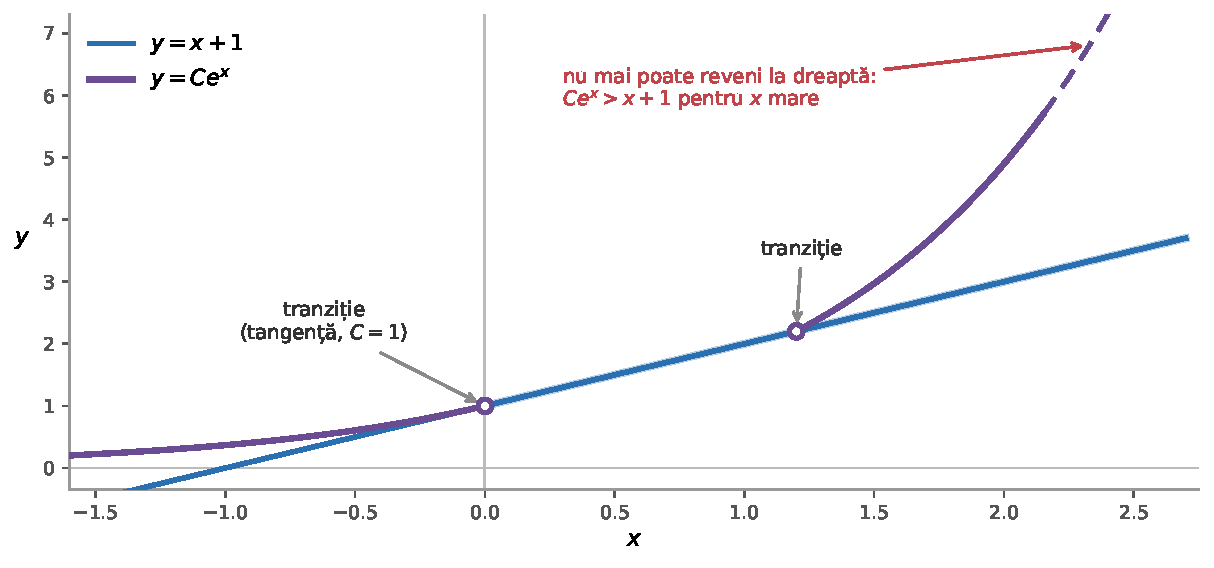
\includegraphics[width=0.86\textwidth]{grafic_p12_nou.pdf}
\caption*{\small\textit{O funcție pe bucăți candidat: alternează între $y=x+1$ (albastru) și $Ce^x$ (mov). Săgețile arată punctele de tranziție. Cheia: odată ce exponențiala depășește dreapta, nu mai poate reveni la ea, deoarece $Ce^x > x+1$ pentru $x$ suficient de mare.}}
\end{figure}

\noindent\textbf{De ce nu funcționează alternarea?} La o tranziție de la exponențial $\to$ liniar trebuie ca $Ce^{x_1} = x_1+1$ și $Ce^{x_1}=1$ (lipire $C^1$), adică tocmai tangența $e^{x_1}\ge x_1+1$, cu egalitate. Singura soluție: $C=1$, $x_1=0$. Dar pentru $x>0$, $e^x > x+1$ strict, deci exponențiala nu mai coboară niciodată la dreaptă. Orice tranziție după $x=0$ este imposibilă. Rămân doar: familia $Ce^x$ (cu $C\ge1$, ca să fie mereu $\ge x+1$) și soluția lipită o singură dată în $x=0$.

\medskip

\emph{Trecerea 2 (redactarea).} Fie $U=\{x:\ f'(x)<x+1\}$ --- mulțime \emph{deschisă}, fiindcă $f'$ e \textbf{continuă} (aici se folosește ipoteza!).

\emph{Pe $U$:} $f(x)=\max(f'(x),x+1)=x+1$, deci, $U$ fiind deschisă, $f'(x)=1$ pe $U$. Dar atunci condiția de apartenență $f'(x)<x+1$ devine $1<x+1$, adică $x>0$: așadar $U\subseteq(0,\infty)$.

\emph{Cazul $U=\varnothing$:} atunci $f'(x)\ge x+1$ peste tot, deci $f(x)=f'(x)$ pentru orice $x$. Ecuația $f'=f$ dă $f(x)=Ce^x$ (prin funcția auxiliară $f(x)e^{-x}$, ca în secțiunea de ecuații diferențiale). Rămâne constrângerea $Ce^x\ge x+1$ pentru orice $x$: pentru $C\le0$ pică în $x=0$; pentru $C>0$, minimul funcției $Ce^x-x-1$ se atinge în $x=-\ln C$ și valorează $\ln C$, deci constrângerea e echivalentă cu $C\ge1$. Obținem familia $f(x)=Ce^x$, $C\ge1$.

\emph{Cazul $U\neq\varnothing$:} fie $(a,b)$ o componentă a lui $U$, cu $0\le a<b\le\infty$. Pe $(a,b)$, $f'\equiv1$; prin continuitatea lui $f'$, $f'(a)=1$. Dar $a\notin U$, deci $f'(a)\ge a+1$, adică $1\ge a+1$, deci $a\le0$: combinat cu $a\ge0$, rezultă $a=0$. Dacă $b<\infty$: la fel $f'(b)=1\ge b+1$, deci $b\le0$ --- contradicție cu $b>0$. Așadar $U=(0,\infty)$, și $f(x)=x+1$ pe $[0,\infty)$ (cu $f(0)=1$ din continuitate). Pe $(-\infty,0]$, complementara lui $U$, avem $f=f'$ (ca mai sus), deci $f(x)=Ce^x$ acolo; $f(0)=1$ dă $C=1$. Verificări finale: lipirea e de clasă $C^1$ ($f'(0-)=e^0=1=f'(0+)$), iar pe $(-\infty,0)$ constrângerea $f'(x)=e^x\ge x+1$ e clasică. \hfill$\blacksquare$

\textbf{Răspuns:} $f(x)=Ce^x$ cu $C\ge1$, \emph{sau} $f(x)=\begin{cases}e^x,&x\le0\\ x+1,&x\ge0.\end{cases}$

\emph{Ce a cumpărat redactarea:} desenul a \emph{ghicit} ambele familii, dar numai argumentul cu mulțimea deschisă $U$ demonstrează că \textbf{nu există altele} --- exact partea invizibilă pe grafic. De remarcat și dicționarul la lucru: „tangenta lui $e^x$ la dreaptă'' $\to$ minimul lui $Ce^x-x-1$ calculat cu derivata; „lipirea merge'' $\to$ verificarea explicită $C^1$; „de la $0$ încolo doar dreapta'' $\to$ argumentul cu capetele componentelor lui $U$.

\subsection{Capcane frecvente (clasa a XI-a)}
\begin{enumerate}[leftmargin=*, itemsep=2pt]
\item Trecerea la limită în recurență cere \emph{mai întâi} demonstrarea convergenței; $\ell=f(\ell)$ singură nu dovedește nimic.
\item Lagrange/Rolle cer continuitate pe intervalul \emph{închis} și derivabilitate pe cel \emph{deschis} --- de verificat explicit ipotezele.
\item Consecințele lui Lagrange (monotonie din semnul derivatei) sunt valabile doar pe \emph{intervale}, nu pe reuniuni de intervale (ex. $-1/x$ are derivată pozitivă pe $\mathbb{R}^*$ dar nu e crescătoare pe $\mathbb{R}^*$).
\item L'Hôpital: de verificat forma nedeterminată și existența limitei raportului derivatelor; implicația nu se inversează.
\item Darboux nu implică continuitate; continuitate implică Darboux.
\item $a_{n+1}-a_n\to 0$ nu implică convergența; $\frac{a_{n+1}}{a_n}\to 1$ nu decide nimic.
\item Punctele de extrem pot fi și în capetele domeniului sau în puncte de nederivabilitate --- Fermat acoperă doar punctele interioare cu derivată.
\item La limite cu $\limsup/\liminf$ sau subșiruri: convergența pe $(x_{2n})$ și $(x_{2n+1})$ trebuie să dea \emph{aceeași} limită.
\end{enumerate}

\subsection{Capcane la integrale (clasa a XII-a)}
\begin{enumerate}[leftmargin=*, itemsep=2pt]
\item „Continuă $\iff$ are primitive'' e fals în ambele rafinări: continuitatea e suficientă dar nu necesară; Darboux e necesară dar nu suficientă.
\item Leibniz--Newton cere ca $G$ să fie primitivă pe \emph{tot} intervalul --- atenție la primitive „pe bucăți'' cu constante nepotrivite la lipire (clasic la $\int\frac{dx}{2+\cos x}$ cu substituția $t=\operatorname{tg}\frac x2$, discontinuă în $\pi$).
\item La schimbarea de variabilă pentru integrale definite se schimbă și capetele; $u$ trebuie să fie derivabilă cu derivata continuă pe intervalul de integrare.
\item $\int_a^b f=0$ nu implică $f\equiv0$ fără ipotezele $f\ge0$ \emph{și} $f$ continuă.
\item Integrabilitatea Riemann cere mărginire; $\int_0^1\frac{dx}{\sqrt x}$ este integrală \emph{improprie}, nu Riemann obișnuită --- se tratează prin limită.
\item În sume Riemann, funcția trebuie să fie integrabilă pe intervalul închis; singularitățile la capete (ca la $x^{-\alpha}$) cer argument suplimentar de trunchiere.
\end{enumerate}

\section{Construcții: ce funcții să încerci}

\emph{Notă:} secțiunea stă la început fiindcă e o \emph{atitudine}, nu un capitol --- se folosește peste tot. Exemplele ei invocă noțiuni tratate riguros mai târziu (derivate, ecuații diferențiale, lipiri pe $\mathbb{Q}$, integrale improprii); la prima citire se pot sări demonstrațiile, reținând reflexele.

Problemele de construcții la ONM sunt, de multe ori, de tipul \emph{„demonstrați că există o funcție cu proprietățile...''} sau \emph{„dați un exemplu de funcție care...''}. Ideea principală: să recunoști rapid \textbf{ce formă de funcție are șanse mari să funcționeze}, apoi să determini parametrii prin calcul direct.

\subsection{Principii generale de construcție}

Problemele de construcție arată la fel în toate ramurile --- combinatorică, teoria numerelor, analiză --- și au un folclor comun de strategii (adaptat aici după materialul „Olympiad Constructions'' al lui Cody Johnson și literatura de combinatorică olimpică):

\begin{enumerate}[leftmargin=*, itemsep=2pt]
\item \textbf{Cazuri mici, întotdeauna primele.} Rezolvă problema pentru $n=1,2,3,4$: cazurile mici îți ghicesc răspunsul (minimul/maximul, forma) și, mai important, îți arată \emph{tiparul} după care se asamblează construcția generală. Echivalentul în analiză: încearcă întâi pe exemplele-jucărie din catalog.
\item \textbf{Construcție prin inducție/asamblare.} Dintr-o construcție de mărime $n$ se fabrică des una de mărime $n+1$ sau $2n$ (dublezi, lipești, adaugi o piesă). În analiză: lipirea funcțiilor pe bucăți ($e^x$ cu $x+1$ la ONM 1994), șirurile de funcții definite recursiv.
\item \textbf{Întâi demonstrează, apoi caută: îngustarea prin restricții.} Înainte de a căuta orbește, demonstrează \emph{proprietăți obligatorii} ale oricărei soluții (în analiză: semne, monotonii, valori forțate în puncte). Fiecare restricție taie din spațiul de căutare --- și de multe ori restricțiile, cumulate, \emph{dictează} construcția. E exact „structura ghicește'' din secțiunile noastre: la $(f')^2+1=f$, compararea gradelor a decis totul înainte de orice încercare.
\item \textbf{La „demonstrați sau infirmați'': atacă serios varianta NU.} Încearcă cu adevărat să demonstrezi imposibilitatea; \emph{locul precis unde argumentul tău eșuează} e harta către construcție --- acolo e libertatea pe care o construcție trebuie s-o exploateze. Și disciplina de concurs: dacă în prima jumătate a timpului n-ai demonstrat „da'', petrece a doua jumătate pe „nu'' --- fără să oscilezi.
\item \textbf{Principiul simplității.} Dacă există o construcție, aproape sigur există una din \emph{piese simple}: mișcări elementare, blocuri repetate, funcții din catalog. Nu căuta obiecte exotice înainte de a epuiza combinațiile banale --- morala tuturor exemplelor din fișă, unde răspunsurile au fost $e^x$, $|x|$, Dirichlet, $\sqrt{x^2+\varepsilon}$, niciodată ceva nemaivăzut.
\end{enumerate}

Restul secțiunii aplică aceste principii la specificul analizei: ce \emph{familii de funcții} joacă rolul „pieselor simple''.

\begin{tehbox}{Reflexul 1: la ecuații funcționale sau diferențiale, încearcă întâi un polinom}

Primul reflex este să presupui că funcția e polinom și să vezi \emph{ce grad ar trebui să aibă}: compararea gradelor spune foarte repede dacă există vreo șansă. Regulile de grad: derivarea scade gradul cu $1$; ridicarea la pătrat îl dublează; compunerea le înmulțește.

\textbf{Exemplu.} Să se construiască $f$ cu $\big(f'(x)\big)^2+1=f(x)$ pentru orice $x$.

\emph{Pasul 1 (gradul).} Dacă $f$ e polinom de grad $n$: $f'$ are grad $n-1$, deci $(f')^2$ are grad $2(n-1)$. Egalitatea gradelor cere $2(n-1)=n$, adică $n=2$. Încercăm $f(x)=ax^2+bx+c$.

\emph{Pasul 2 (calcul direct).} $f'(x)=2ax+b$, deci
\[
(2ax+b)^2+1=ax^2+bx+c
\quad\Longleftrightarrow\quad
4a^2x^2+4abx+b^2+1=ax^2+bx+c,
\]
și identificarea coeficienților dă sistemul $4a^2=a$, $4ab=b$, $b^2+1=c$.

\emph{Pasul 3 (rezolvarea).} Din prima: $a=0$ (pierde gradul 2) sau $a=\frac14$. Pentru $a=\frac14$, a doua ecuație devine $b\cdot0=0$, deci $b$ e \emph{arbitrar}, iar $c=b^2+1$:
\[
\boxed{\ f(x)=\frac{x^2}{4}+bx+b^2+1,\qquad b\in\mathbb{R}.\ }
\]
Verificare: $f'(x)=\frac x2+b$, $\big(\frac x2+b\big)^2+1=\frac{x^2}4+bx+b^2+1=f(x)$. \checkmark

\end{tehbox}

\subsection{Reflexul 2: condiția $f>0$ pe tot domeniul}

Când enunțul cere $f(x)>0$ pentru orice $x$ din domeniu (de obicei $(0,\infty)$), formele naturale de testat sunt
\[
f(x)=c_2\,x^{c_1}\qquad\text{și}\qquad f(x)=b\cdot a^{x},
\]
cu $c_2,b>0$ --- puterile și exponențialele sunt pozitivele „canonice'' și se comportă perfect la înmulțiri, compuneri și derivări (rămân în aceeași familie). Nu întâmplător: acestea sunt exact soluțiile ecuațiilor funcționale clasice (secțiunea de ecuații Cauchy), deci orice condiție cu structură multiplicativă le va selecta.

\subsection{Reflexul 3: discontinuități controlate --- funcții de tip Dirichlet}

Când trebuie construită o funcție cu un număr \emph{controlat} de puncte de discontinuitate sau de nederivabilitate, ideea standard este definirea diferită pe $\mathbb{Q}$ și pe $\mathbb{R}\setminus\mathbb{Q}$. Instrumentul teoretic e deja în fișă (subsecțiunea „Funcții definite prin cazuri pe $\mathbb{Q}$ și $\mathbb{R}\setminus\mathbb{Q}$''): pentru $g,h$ continue, funcția lipită e \textbf{continuă exact în punctele unde $g(x)=h(x)$}, și derivabilă exact unde ramurile se ating cu tot cu derivate. Construcția devine astfel o \emph{ecuație}: vrei discontinuitate exact pe o mulțime $S$? Alege ramuri care coincid exact pe complementara lui $S$.

\subsection{Reflexul 4: Ce funcții clasice care verifică ipoteza știu?}

Înainte de a inventa ceva complicat, pune-ți întrebarea: \emph{„ce exemplu cu proprietățile acestea știu deja?''} Subpunctele de tip „dați un exemplu / rezultă că...?'' de la olimpiadă se rezolvă aproape întotdeauna dintr-un catalog scurt, combinat cu mici ajustări (translații, înmulțiri cu constante, $x^2+\varepsilon$ în loc de $x^2$):

\begin{enumerate}[leftmargin=*, itemsep=2pt]
\item \textbf{Dirichlet} $\mathbf{1}_{\mathbb{Q}}$ --- discontinuă peste tot; $x\cdot\mathbf{1}_{\mathbb{Q}}$ --- continuă doar în $0$; $x$ pe $\mathbb{Q}$, $x+1$ în rest --- discontinuă peste tot dar cu limite „pe ramuri''.
\item $|x|$ --- continuă, nederivabilă într-un punct; $\sqrt{x^2+\varepsilon}$ --- neteda care o aproximează.
\item $\sin\frac1x$ --- mărginită fără limită în $0$; $x\sin\frac1x$ --- continuă, nederivabilă în $0$; $x^2\sin\frac1x$ --- derivabilă cu derivata discontinuă.
\item $x^3$ --- strict crescătoare cu derivata nulă într-un punct; $x+2\sin x$ --- derivată care schimbă semnul de infinite ori, dar funcția $\to\infty$.
\end{enumerate}

Morala: la punctele b) de tip „rezultă că...?'', răspunsul „nu'' se demonstrează cu un membru al catalogului, ajustat minimal.

\subsection*{Exemplu}

\emph{Fie $f:\mathbb{R}\to\mathbb{R}$ pentru care există o funcție derivabilă $g:\mathbb{R}\to\mathbb{R}$ și un șir $(a_n)$ de numere strict pozitive, convergent la $0$, astfel încât}
\[
g'(x)=\lim_{n\to\infty}\frac{f(x+a_n)-f(x)}{a_n}\qquad\forall x\in\mathbb{R}.
\]
\emph{a) Dați un exemplu de astfel de $f$ care nu e derivabilă în niciun punct.}

\emph{Soluție.} Gândim simplu: ne trebuie o funcție nederivabilă peste tot --- primul candidat din catalog e Dirichlet, $f=\mathbf{1}_{\mathbb{Q}}$. Verificăm că merge cu $a_n=\frac1n$: dacă $x\in\mathbb{Q}$, atunci $x+\frac1n\in\mathbb{Q}$; dacă $x\notin\mathbb{Q}$, atunci $x+\frac1n\notin\mathbb{Q}$ --- adunarea unui rațional \emph{păstrează clasa}. Deci
\[
f\Big(x+\frac1n\Big)=f(x)\quad\forall x,n
\qquad\Longrightarrow\qquad
\frac{f(x+a_n)-f(x)}{a_n}=0\to0,
\]
așa că ipoteza e satisfăcută cu $g$ constantă ($g'\equiv0$). Iar $f$ e discontinuă în orice punct (ramurile constante $1$ și $0$ nu se ating nicăieri --- corolarul lipirii), deci nederivabilă peste tot. $\blacksquare$

\emph{De reținut:} toată soluția stă în alegerea șirului $a_n$ \emph{rațional} --- limita pe un șir particular nu vede structura fină a funcției. Exact acest fenomen face ca punctul b) al problemei (dacă $f$ e \emph{continuă}, atunci e derivabilă) să fie partea grea.

\subsection*{Exemplu: ONM 2026, etapa națională, clasa a XI-a, Problema 1b)}

\textbf{Enunț.} Fie $h:\mathbb{R}\to\mathbb{R}$ o funcție continuă și $(f_n)$, $(g_n)$ două șiruri de funcții derivabile cu proprietatea că $f_n(x)<h(x)<g_n(x)$ pentru orice $x\in\mathbb{R}$ și orice $n\in\mathbb{N}^*$, și că $g_n(x)-f_n(x)\to0$ pentru orice $x\in\mathbb{R}$. Este $h$ neapărat derivabilă?

\textbf{Răspuns: NU.}

Am participat la ONM 2026 și acesta a fost raționamentul meu la această problemă.

\emph{Cum se ghicește contraexemplul.} În timpul concursului am desenat un grafic. Condițiile problemei spun că $h$ e prinsă între două familii de funcții derivabile care o strivesc --- pe grafic asta înseamnă două „clești'' de curbe netede care coboară și urcă spre $h$ din ambele părți. Singura funcție continuă și nederivabilă pe care o știam era $h(x)=|x|$ --- are un colț în $0$, dar e altfel perfect inofensivă. Am desenat-o și am căutat cu ochii niște curbe derivabile, mai sus și mai jos, care să o strângă:

\begin{center}
\begin{tikzpicture}[scale=2.0, >=latex]
  % Axe
  \draw[->] (-1.30,0) -- (1.32,0) node[right] {$x$};
  \draw[->] (0,-0.50) -- (0,1.28) node[above] {$y$};
  \node[below left, font=\small] at (0,0) {$0$};

  % Curbe de sus -- violet, intrerupte
  \draw[onm!35, line width=0.85pt, dashed, domain=-1.28:1.28, samples=100]
    plot (\x, {sqrt(\x*\x + 1)});
  \draw[onm!65, line width=1pt, dashed, domain=-1.28:1.28, samples=100]
    plot (\x, {sqrt(\x*\x + 0.25)});
  \draw[onm, line width=1.3pt, dashed, domain=-1.28:1.28, samples=100]
    plot (\x, {sqrt(\x*\x + 0.04)});

  % Curbe de jos -- portocaliu, punctate, coboara sub 0
  \draw[ojm!35, line width=0.85pt, dotted, domain=-1.28:1.28, samples=100]
    plot (\x, {sqrt(\x*\x + 1) - 1.4142});
  \draw[ojm!65, line width=1pt, dotted, domain=-1.28:1.28, samples=100]
    plot (\x, {sqrt(\x*\x + 0.25) - 0.7071});
  \draw[ojm, line width=1.3pt, dotted, domain=-1.28:1.28, samples=100]
    plot (\x, {sqrt(\x*\x + 0.04) - 0.2828});

  % |x| -- linie groasa, desenata dupa curbe ca sa fie deasupra
  \draw[ink, line width=2.4pt, domain=-1.28:0, samples=2]
    plot (\x, {-\x});
  \draw[ink, line width=2.4pt, domain=0:1.28, samples=2]
    plot (\x, {\x});

  % Eticheta h(x) -- in interiorul graficului, la stanga
  \node[ink, font=\small\bfseries, fill=white, inner sep=1pt]
    at (-0.75, 0.88) {$h(x)=|x|$};

  % Punct de colt
  \filldraw[ink] (0,0) circle (0.030);
  \node[ink, above right, font=\small] at (0.05, 0.04) {colț};

  % Etichete sus/jos
  \node[onm, font=\scriptsize\itshape] at (0.60, 1.15) {sus};
  \node[ojm, font=\scriptsize\itshape] at (0.75, 0.55) {jos};
\end{tikzpicture}
\end{center}

Forma curbelor de deasupra mi-a sugerat imediat o hiperbolă netezită. Odată ales $h$ și observat că curbele seamănă cu $\sqrt{x^2+\varepsilon}$, am ales formal:

\textbf{Construcția.} Punem
\[
g_n(x)=\sqrt{x^2+\tfrac1n},\qquad f_n(x)=\sqrt{x^2+\tfrac1n}-\sqrt{\tfrac2n}.
\]
\emph{Derivabilitate:} $x^2+\frac1n>0$, deci ambele sunt $C^\infty$ pe $\mathbb{R}$.

\emph{Încadrarea $f_n<h<g_n$:} Inegalitatea $g_n>|x|$ e clară. Inegalitatea $f_n<|x|$ revine la $\sqrt{x^2+\frac1n}-\sqrt{\frac2n}<|x|$, adică (ridicând la pătrat, ambii membri nenegativi pentru $n$ mare):
\[
x^2+\frac1n < x^2+2|x|\sqrt{\tfrac2n}+\frac2n
\quad\Longleftrightarrow\quad
0 < 2|x|\sqrt{\tfrac2n}+\frac1n,
\]
adevărată pentru orice $x\in\mathbb{R}$.

\emph{Strângerea:} $g_n(x)-f_n(x)=\sqrt{\frac2n}\to0$ uniform.

Toate ipotezele sunt satisfăcute, dar $h=|x|$ nu e derivabilă în $0$. $\blacksquare$



\chapter{Clasa a XII-a}

\section{Primitive}

\begin{definitie}
$F$ este \textbf{primitivă} a lui $f$ pe intervalul $I$ dacă $F$ e derivabilă pe $I$ și $F'=f$. Mulțimea primitivelor este $\int f(x)\,dx=F(x)+\mathcal{C}$: două primitive diferă printr-o constantă \emph{pe interval} (consecința lui Lagrange).
\end{definitie}

\begin{teorema}[Existența]
Orice funcție \textbf{continuă} pe un interval admite primitive. Reciproc \textbf{nu}: există funcții discontinue cu primitive (ex. $f(x)=2x\sin\frac1x-\cos\frac1x$ pentru $x \neq 0$, $f(0)=0$, e discontinuă în $0$, dar are primitiva $F(x)=x^2\sin\frac1x$ pentru $x\neq0$, $F(0)=0$).
\end{teorema}

\begin{teorema}[Obstrucția Darboux]
Dacă $f$ admite primitive pe $I$, atunci $f$ are proprietatea lui Darboux pe $I$ (fiind derivata unei funcții --- Teorema Darboux din Partea I). Consecință practică: o funcție care \emph{nu} are Darboux (ex. cu o discontinuitate de speța I, sau cu $f(I)$ ne-interval) \textbf{nu admite primitive}. Acesta e testul standard la problemele „arătați că $f$ nu admite primitive''.
\end{teorema}

\begin{obs}
Atenție: Darboux e condiție \emph{necesară}, nu suficientă --- există funcții cu proprietatea Darboux fără primitive. La probleme de existență se folosesc frecvent: descompunerea $f=g+h$ cu $g$ continuă (are primitive) și analiza lui $h$; sau argumentul cu limita $\frac{F(x)-F(0)}{x}$ în puncte problematice.
\end{obs}

\begin{teorema}[Integrarea prin părți]
Dacă $f,g:I\to\mathbb{R}$ sunt derivabile cu derivatele continue, atunci $f'g$ și $fg'$ admit primitive pe $I$ și
\[
\int f(x)\,g'(x)\,dx=f(x)\,g(x)-\int f'(x)\,g(x)\,dx.
\]
\end{teorema}

\begin{teorema}[Prima schimbare de variabilă]
Fie $\varphi:I\to J$ derivabilă și $h:J\to\mathbb{R}$ cu primitive ($H$ una dintre ele). Atunci $(h\circ\varphi)\cdot\varphi'$ admite primitive pe $I$ și
\[
\int h\big(\varphi(x)\big)\,\varphi'(x)\,dx=H\big(\varphi(x)\big)+\mathcal C.
\]
Practic: fiecare linie din tabelul de mai jos are automat o „versiune compusă'' --- se înlocuiește $x$ cu $\varphi(x)$ și se cere factorul $\varphi'(x)$ sub integrală (de aceea nu mai listăm separat tabelul compus).
\end{teorema}

\begin{teorema}[A doua schimbare de variabilă]
Fie $\varphi:I\to J$ \textbf{bijectivă}, derivabilă, cu $\varphi'(x)\neq0$ pe $I$, și $f:J\to\mathbb{R}$. Dacă $h=(f\circ\varphi)\cdot\varphi'$ admite primitive pe $I$ (fie $H$ una), atunci $f$ admite primitive pe $J$ și
\[
\int f(x)\,dx=\big(H\circ\varphi^{-1}\big)(x)+\mathcal C.
\]
Deosebirea de prima: acolo recunoști în integrand tiparul $h(\varphi)\varphi'$ gata format; aici \emph{tu} introduci substituția $x=\varphi(t)$ și, la final, revii prin $\varphi^{-1}$ --- de aceea e nevoie de bijectivitate.
\end{teorema}


\medskip
\textbf{Exemplu.} $\displaystyle\int \frac{\cos x}{1+\sin^2 x}\,dx$.

Recunoaștem tiparul $h(\varphi)\cdot\varphi'$ cu $\varphi(x)=\sin x$ (deci $\varphi'(x)=\cos x$) și $h(t)=\dfrac{1}{1+t^2}$, a cărei primitivă e $H(t)=\mathrm{arctg}\,t$. Aplicând direct teorema:
\[
\int \frac{\cos x}{1+\sin^2 x}\,dx = \mathrm{arctg}(\sin x)+\mathcal C.
\]

\medskip
\textbf{Exemplu.} $\displaystyle\int \sqrt{1-x^2}\,dx$.

Lucrăm întâi pe $(-1,1)$. Introducem $x=\sin t$, $t\in\bigl(-\frac\pi2,\frac\pi2\bigr)$ (bijecție pe $(-1,1)$, cu $\varphi'(t)=\cos t>0$; în capetele $\pm\frac\pi2$ derivata s-ar anula, de aceea le excludem). Atunci $\sqrt{1-x^2}=\cos t$ și $dx=\cos t\,dt$:
\[
\int \sqrt{1-x^2}\,dx = \int \cos^2 t\,dt = \frac{t+\sin t\cos t}{2}+\mathcal C.
\]
Revenind prin $\varphi^{-1}$: $t=\arcsin x$, $\sin t=x$, $\cos t=\sqrt{1-x^2}$, deci
\[
\int \sqrt{1-x^2}\,dx = \frac{\arcsin x + x\sqrt{1-x^2}}{2}+\mathcal C.
\]
Formula rămâne valabilă pe tot $[-1,1]$: funcția din dreapta e continuă pe $[-1,1]$, iar derivata ei, $\sqrt{1-x^2}$, are limita $0$ în $\pm1$; prin corolarul teoremei lui Lagrange, e derivabilă și în capete, cu derivata $0=\sqrt{1-(\pm1)^2}$.

{Tabelul primitivelor uzuale (pe intervale pe care expresiile au sens)}
\[
\renewcommand{\arraystretch}{1.55}\setlength{\arraycolsep}{3pt}
\begin{array}{ll|ll}
\displaystyle\int x^{a}\,dx=\frac{x^{a+1}}{a+1}+\mathcal C\ (a\neq-1) &&
\displaystyle\int \frac{dx}{x}=\ln|x|+\mathcal C &\\[2pt]
\displaystyle\int a^{x}\,dx=\frac{a^{x}}{\ln a}+\mathcal C\ \ (e^x\mapsto e^x) &&
\displaystyle\int \frac{dx}{x^{2}+a^{2}}=\frac1a\,\mathrm{arctg}\,\frac xa+\mathcal C &\\[2pt]
\displaystyle\int \frac{dx}{x^{2}-a^{2}}=\frac{1}{2a}\ln\Big|\frac{x-a}{x+a}\Big|+\mathcal C &&
\displaystyle\int \frac{dx}{\sqrt{a^{2}-x^{2}}}=\arcsin\frac xa+\mathcal C &\\[2pt]
\displaystyle\int \frac{dx}{\sqrt{x^{2}\pm a^{2}}}=\ln\big|x+\sqrt{x^{2}\pm a^{2}}\big|+\mathcal C &&
\displaystyle\int \sin x\,dx=-\cos x+\mathcal C &\\[2pt]
\displaystyle\int \cos x\,dx=\sin x+\mathcal C &&
\displaystyle\int \frac{dx}{\cos^{2}x}=\mathrm{tg}\,x+\mathcal C &\\[2pt]
\displaystyle\int \frac{dx}{\sin^{2}x}=-\mathrm{ctg}\,x+\mathcal C &&
\displaystyle\int \mathrm{tg}\,x\,dx=-\ln|\cos x|+\mathcal C &\\[2pt]
\displaystyle\int \mathrm{ctg}\,x\,dx=\ln|\sin x|+\mathcal C &&
\displaystyle\int \mathrm{sh}\,x\,dx=\mathrm{ch}\,x+\mathcal C &\\[2pt]
\displaystyle\int \mathrm{ch}\,x\,dx=\mathrm{sh}\,x+\mathcal C && &
\end{array}
\]
Atenție la redactare: domeniul contează. De pildă, $\frac1x$ are primitiva $\ln x$ pe $(0,\infty)$ și $\ln(-x)$ pe $(-\infty,0)$, cu constante \emph{independente} pe cele două intervale (capcana „constantelor pe bucăți'' din secțiunea de redactare).


\begin{teorema}[Descompunerea în fracții simple]
Fracțiile raționale \textbf{simple} sunt: polinoamele, $\dfrac{A}{(x-a)^{n}}$ și $\dfrac{Bx+C}{(x^{2}+bx+c)^{n}}$ cu $b^{2}-4c<0$. Orice funcție rațională $\frac{P}{Q}$ se scrie \emph{unic} ca sumă finită de fracții simple: partea polinomială (câtul împărțirii, dacă $\deg P\ge\deg Q$) plus, pentru fiecare factor $(x-a)^{\alpha}$ al lui $Q$, termenii $\frac{A_1}{x-a}+\dots+\frac{A_\alpha}{(x-a)^{\alpha}}$, și pentru fiecare factor $(x^{2}+bx+c)^{\beta}$ ireductibil (adică $b^2-4c<0$: nu se descompune în factori de gradul întâi cu coeficienți reali), termenii $\frac{B_1x+C_1}{x^{2}+bx+c}+\dots+\frac{B_\beta x+C_\beta}{(x^{2}+bx+c)^{\beta}}$.
\end{teorema}

\begin{tehbox}{Rețeta de integrare a unei funcții raționale}
\begin{enumerate}[leftmargin=*, itemsep=1pt]
\item Dacă $\deg P\ge\deg Q$: împărțire cu rest --- partea polinomială se integrează direct.
\item Descompune în fracții simple (coeficienții: identificare sau valori particulare $x=a$).
\item $\displaystyle\int\frac{A\,dx}{(x-a)^{n}}$: direct din tabel (logaritm pentru $n=1$, putere pentru $n\ge2$).
\item $\displaystyle\int\frac{Bx+C}{x^{2}+bx+c}\,dx$: scrie numărătorul ca $\frac B2(2x+b)+\big(C-\frac{Bb}{2}\big)$ --- prima bucată dă $\frac B2\ln(x^{2}+bx+c)$ (derivata numitorului!), a doua, după forma canonică $\big(x+\frac b2\big)^{2}+\big(c-\frac{b^{2}}4\big)$, dă un $\mathrm{arctg}$.
\item Puterile $\ge2$ ale trinomului: recurență prin părți --- același mecanism ca în secțiunea de recurențe de integrale.
\end{enumerate}
\end{tehbox}

\subsection{Structura mulțimii funcțiilor cu primitive}

Notăm, pentru un interval nedegenerat $J$: $C(J)=$ funcțiile continue, $P(J)=$ funcțiile care admit primitive, $Da(J)=$ funcțiile cu proprietatea lui Darboux. Cele două teoreme de mai sus se rezumă într-o diagramă de reținut:
\[
C(J)\ \subsetneq\ P(J)\ \subsetneq\ Da(J),
\]
\textbf{ambele incluziuni fiind stricte}. Vizual:

\begin{center}
\begin{tikzpicture}[scale=0.92]
\draw[rounded corners=14pt, thick, fill=orange!8] (-5.1,-2.05) rectangle (5.1,2.05);
\draw[rounded corners=12pt, thick, fill=orange!20] (-3.55,-1.45) rectangle (3.55,1.45);
\draw[rounded corners=10pt, thick, fill=orange!38] (-2.0,-0.85) rectangle (2.0,0.85);
\node at (0,0.45) {\textbf{$C(J)$: continue}};
\node at (0,-0.15) {\footnotesize polinoame, $e^x$, $\sin$, \dots};
\node at (0,1.12) {\textbf{$P(J)$: cu primitive}};
\node at (0,1.72) {\textbf{$Da(J)$: cu proprietatea Darboux}};
\node at (0,-1.15) {\footnotesize $f_0=\sin\frac1x$ (cu $0$ în $0$): în $P\setminus C$};
\node at (0,-1.78) {\footnotesize $f_a=\sin\frac1x$ (cu $a\neq0$, $|a|\le1$, în $0$): în $Da\setminus P$};
\end{tikzpicture}
\end{center}

Martorii stricteții sunt amândoi din aceeași familie:

\begin{teorema}[Familia $\sin\frac1x$, clasificată complet]
Fie $a\in\mathbb{R}$ și $f_a:\mathbb{R}\to\mathbb{R}$, $f_a(x)=\sin\frac1x$ pentru $x\neq0$, $f_a(0)=a$. Atunci:
\[
f_a\ \text{admite primitive pe }\mathbb{R}\quad\Longleftrightarrow\quad a=0.
\]
În particular: $f_0\in P(\mathbb{R})\setminus C(\mathbb{R})$ (prima strictețe), iar $f_a$ cu $a\in[-1,1]$, $a\neq0$, are Darboux dar nu are primitive: $f_a\in Da(\mathbb{R})\setminus P(\mathbb{R})$ (a doua strictețe).
\end{teorema}
\begin{proof}
\emph{$a=0$ merge:} funcția $G(x)=x^2\cos\frac1x$, $G(0)=0$, e derivabilă peste tot, cu
\[
G'(x)=2x\cos\frac1x+\sin\frac1x\ \ (x\neq0),\qquad G'(0)=\lim_{x\to0}\frac{x^2\cos\frac1x}{x}=0.
\]
Deci $f_0(x)=G'(x)-2x\cos\frac1x$: diferență dintre o derivată și o funcție \emph{continuă} (prelungită cu $0$ în origine) --- ambele admit primitive, deci și $f_0$ (combinațiile liniare de funcții cu primitive au primitive).

\emph{$a\neq0$ nu merge:} prin absurd, dacă $f_a$ ar avea primitive, atunci $f_a-f_0$ ar avea primitive (diferență). Dar $f_a-f_0$ e funcția egală cu $a$ în $0$ și cu $0$ în rest --- imaginea ei e $\{0,a\}$, care nu e interval, deci nu are Darboux, deci nu are primitive. Contradicție.

\emph{Darboux pentru $a\in[-1,1]$:} pe orice interval care conține $0$, $f_a$ ia toate valorile din $[-1,1]$ (oscilația lui $\sin\frac1x$), deci imaginea oricărui interval e interval.
\end{proof}

\begin{obs}
Schema de demonstrație merită reținută ca metodă: (1) pentru a arăta că o funcție oscilantă \emph{are} primitive, o scrii ca $G'-(\text{ceva continuu})$ cu $G$ construit „cu un $x^2$ în față''; (2) pentru a arăta că \emph{nu} are, o compari prin diferență cu una care are --- spațiul $P(J)$ fiind închis la combinații liniare, obstrucția cade pe diferență, unde criteriile Darboux mușcă.
\end{obs}

\begin{teorema}[Produse de funcții cu primitive]
Produsul a două funcții cu primitive \textbf{nu} are, în general, primitive. Condiții suficiente ca $f\cdot g$ să admită primitive pe $J$:
\begin{enumerate}[leftmargin=*, itemsep=2pt]
\item $f$ admite primitive și $g$ e \textbf{derivabilă cu derivata continuă} ($g\in C^1$);
\item \emph{(Wilkosz)} $f$ admite primitive și e \textbf{mărginită} (superior sau inferior), iar $g$ e \textbf{continuă};
\item $f$ admite primitive și $g$ e derivabilă cu \textbf{derivata mărginită};
\item $f$ admite primitive, $f(x)\neq0$ pe $J$, iar $g$ e continuă.
\end{enumerate}
\end{teorema}
\begin{proof}[Demonstrația punctului 1 (și de ce 3 decurge din 2)]
Fie $F$ o primitivă a lui $f$. Din regula produsului, $(Fg)'=fg+Fg'$, deci
\[
f g=(Fg)'-F\,g'.
\]
Primul termen e o derivată (are primitive prin definiție); al doilea, $Fg'$, e \emph{continuu} ($F$ derivabilă deci continuă, $g'$ continuă), deci are primitive prin teorema de existență. Diferența are primitive. $\square$ \quad Pentru punctul 3, același truc reduce totul la primitivabilitatea lui $Fg'$: acum $g'$ e o derivată (deci are primitive) \emph{mărginită}, iar $F$ e continuă --- exact ipotezele lui Wilkosz cu rolurile $f\leftrightarrow g$ schimbate. Punctele 2 și 4 se citează ca atare.
\end{proof}

\textbf{Exemple rezolvate.} \emph{(a)} $h(x)=\ln(x^2+4)\cdot\sin\frac1x$ pentru $x\neq0$, $h(0)=0$, are primitive pe $\mathbb{R}$: ia $f=f_0$ (are primitive, prin teorema familiei; mărginită de $1$) și $g(x)=\ln(x^2+4)$ continuă --- Wilkosz. \emph{(b)} $h(x)=|x-a^2|\cdot\sin\frac1x$, $h(0)=0$: la fel, $g(x)=|x-a^2|$ e doar continuă (nu $C^1$ în $a^2$!), deci punctul 1 nu se aplică --- dar Wilkosz da. Acesta e și motivul pentru care Wilkosz merită știut: salvează exact cazurile cu $g$ continuă neneted.

\begin{teorema}[Câturi și compuneri, enunțuri]
\emph{(Jarník)} Dacă $f,g$ admit primitive pe $J$ și $g(x)\neq0$ pe $J$, atunci câtul $\frac fg$ are \textbf{proprietatea lui Darboux} pe $J$ --- dar poate să \emph{nu} admită primitive: pentru
\[
f(x)=8+\sin^3\tfrac1x,\quad g(x)=2+\sin\tfrac1x\ \ (x\neq0),\qquad f(0)=8,\ g(0)=2,
\]
ambele admit primitive pe $\mathbb{R}$, iar $\frac fg$ nu. \emph{(Compunerea)} Dacă $f:\mathbb{R}\to\mathbb{R}$ admite primitive, iar $g:J\to\mathbb{R}$ e de două ori derivabilă cu $g''$ continuă și $g'(x)\neq0$ pe $J$, atunci $f\circ g$ admite primitive pe $J$. (Motivul: dacă $F$ e o primitivă a lui $f$, atunci $f\circ g=(F\circ g)'\cdot\frac1{g'}$, iar $\frac1{g'}$ e de clasă $C^1$; se aplică punctul 1 al teoremei despre produse.) Exemplu-tip: dacă $f$ admite primitive pe $\mathbb{R}$, atunci și $x\mapsto f\big(x^3+x\big)$ admite, fiindcă $g(x)=x^3+x$ are $g'(x)=3x^2+1\neq0$ și $g''(x)=6x$ continuă.
\end{teorema}

\begin{obs}
Morala practică a întregii subsecțiuni: $P(J)$ e închis la sume și înmulțiri cu scalari, dar \textbf{nu} la produse, câturi sau compuneri --- fiecare operație cere o ipoteză suplimentară de regularitate pe unul dintre factori ($C^1$, mărginire, derivată mărginită). La problemele „arătați că $h$ admite primitive'' cu $h$ oscilant în jurul unui punct, drumul e aproape întotdeauna: desparte $h$ în (derivată explicită) $+$ (parte continuă), sau aplică Wilkosz cu factorizarea potrivită.
\end{obs}

\section{Integrala Riemann}

\begin{definitie}
Pentru o diviziune $\Delta: a=x_0<x_1<\dots<x_n=b$ cu norma $\|\Delta\|=\max(x_i-x_{i-1})$ și puncte intermediare $\xi_i\in[x_{i-1},x_i]$, suma Riemann este $\sigma_\Delta(f;\xi)=\sum_i f(\xi_i)(x_i-x_{i-1})$. Funcția $f$ este \textbf{integrabilă Riemann} pe $[a,b]$ dacă $\sigma_\Delta(f;\xi)$ tinde la un număr $\int_a^b f(x)\,dx$ când $\|\Delta\|\to 0$, indiferent de alegerea punctelor intermediare.
\end{definitie}

\begin{teorema}[Caracterizarea cu șiruri de diviziuni]
$f$ e integrabilă Riemann pe $[a,b]$ dacă și numai dacă pentru \emph{orice} șir de diviziuni $(\Delta_n)$ cu $\|\Delta_n\|\to0$ și orice alegeri de puncte intermediare $\xi^n$, șirul sumelor Riemann $\big(\sigma_{\Delta_n}(f;\xi^n)\big)$ converge; toate aceste limite coincid atunci cu $\int_a^b f$. Aceasta e versiunea „Heine'' a definiției --- și exact teorema care legitimează calculul limitelor de tipul $\frac1n\sum f\big(\frac kn\big)\to\int_0^1f$ din Partea a II-a: diviziunile echidistante sunt un șir particular cu norma $\frac1n\to0$.
\end{teorema}

\begin{teorema}[Proprietăți fundamentale]
Fie $f,g$ integrabile pe $[a,b]$ și $\lambda,\mu\in\mathbb{R}$. Atunci:
\begin{enumerate}[leftmargin=*, itemsep=1pt]
\item \textbf{Liniaritate:} $\lambda f+\mu g$ e integrabilă și $\int_a^b(\lambda f+\mu g)=\lambda\int_a^b f+\mu\int_a^b g$.
\item \textbf{Aditivitate (Chasles):} pentru $c\in(a,b)$, $\int_a^b f=\int_a^c f+\int_c^b f$; cu convențiile $\int_a^a f=0$ și $\int_b^a f=-\int_a^b f$, relația are loc pentru orice așezare a punctelor $a,b,c$.
\item \textbf{Monotonie:} dacă $f\le g$ pe $[a,b]$, atunci $\int_a^b f\le\int_a^b g$; în particular $\Big|\int_a^b f\Big|\le\int_a^b|f|\le(b-a)\sup|f|$ --- estimarea de bază a întregii teorii. Tot de aici: dacă $m\le f\le M$ pe $[a,b]$, atunci $m(b-a)\le\int_a^b f\le M(b-a)$.
\end{enumerate}
\end{teorema}

\begin{teorema}[Clase de funcții integrabile]
Sunt integrabile pe $[a,b]$: funcțiile continue; funcțiile monotone; funcțiile mărginite cu un număr finit de puncte de discontinuitate. Orice funcție integrabilă este mărginită. Modificarea lui $f$ într-un număr finit de puncte nu schimbă integrala.
\end{teorema}

\begin{teorema}[Criteriul lui Darboux]
Fie $f$ mărginită pe $[a,b]$. Pentru o diviziune $\Delta$, notăm cu $m_i,M_i$ infimumul și supremumul lui $f$ pe $[x_{i-1},x_i]$ și definim \textbf{sumele Darboux}
\[
\begin{aligned}
s(\Delta)&=\sum_i m_i\,(x_i-x_{i-1})\qquad\text{(inferioară)},\\
S(\Delta)&=\sum_i M_i\,(x_i-x_{i-1})\qquad\text{(superioară)},
\end{aligned}
\]
care încadrează orice sumă Riemann pe $\Delta$: $s(\Delta)\le\sigma_\Delta(f;\xi)\le S(\Delta)$. Atunci:
\[
f\ \text{integrabilă Riemann}\quad\Longleftrightarrow\quad
\forall\varepsilon>0\ \ \exists\,\Delta:\ \ S(\Delta)-s(\Delta)<\varepsilon.
\]
\end{teorema}

\begin{obs}[Cum se folosește criteriul]
Diferența $S(\Delta)-s(\Delta)=\sum_i(M_i-m_i)(x_i-x_{i-1})$ măsoară „oscilația totală'' a lui $f$ pe diviziune; criteriul spune că integrabilitatea $=$ oscilația poate fi făcută oricât de mică. Cele două clase mari ies în câte două rânduri:
\emph{monotonă} ($f$ crescătoare): $M_i-m_i=f(x_i)-f(x_{i-1})$, deci pentru diviziunea echidistantă cu pas $h$,
$S-s=h\sum_i\big(f(x_i)-f(x_{i-1})\big)=h\big(f(b)-f(a)\big)\to0$ (sumă telescopică!);
\emph{continuă}: prin teorema lui Cantor (Partea I), $f$ e \emph{uniform} continuă, deci pentru pas suficient de mic toate oscilațiile $M_i-m_i<\frac{\varepsilon}{b-a}$, și $S-s<\varepsilon$. Criteriul Darboux e, la olimpiadă, unealta standard pentru „arătați că $f$ e (sau nu e) integrabilă''.
\end{obs}

\begin{definitie}[Mulțime neglijabilă]
Intuiția: o mulțime $N\subset\mathbb{R}$ e „neglijabilă'' dacă poate fi \emph{ascunsă} sub o colecție de intervale a căror lungime totală e oricât de mică vrem. Formal: $N$ este \textbf{neglijabilă} dacă pentru orice $\varepsilon>0$ există intervale deschise $I_1,I_2,I_3,\dots$ (un șir, eventual finit) astfel încât
\[
N\subseteq I_1\cup I_2\cup I_3\cup\dots
\qquad\text{și}\qquad
\ell(I_1)+\ell(I_2)+\ell(I_3)+\dots<\varepsilon,
\]
unde $\ell(I)$ e lungimea intervalului $I$ (suma fiind o serie convergentă, dacă intervalele sunt o infinitate).

Să o simțim pe exemple, de la simplu la interesant:
\begin{enumerate}[leftmargin=*, itemsep=2pt]
\item \textbf{Un punct} $\{a\}$: îl acoperim cu $\big(a-\frac\varepsilon4,\,a+\frac\varepsilon4\big)$, de lungime $\frac\varepsilon2<\varepsilon$. Neglijabil.
\item \textbf{O mulțime finită} $\{a_1,\dots,a_k\}$: câte un interval de lungime $\frac{\varepsilon}{2k}$ în jurul fiecărui punct; lungime totală $\frac\varepsilon2<\varepsilon$. Neglijabilă.
\item \textbf{O mulțime numărabilă} $\{a_1,a_2,a_3,\dots\}$ (de pildă $\mathbb{Q}$!): aici e trucul frumos --- nu mai putem da tuturor aceeași lungime, dar putem da lungimi care \emph{scad geometric}: pe $a_n$ îl acoperim cu un interval de lungime $\dfrac{\varepsilon}{2^{n+1}}$. Lungimea totală:
\[
\sum_{n=1}^{\infty}\frac{\varepsilon}{2^{n+1}}=\frac{\varepsilon}{2}<\varepsilon.
\]
Deci \textbf{orice mulțime cel mult numărabilă e neglijabilă} --- inclusiv $\mathbb{Q}$, deși $\mathbb{Q}$ e densă în $\mathbb{R}$! Densitatea și „mărimea'' sunt lucruri diferite.
\item \textbf{Un interval $[a,b]$ cu $a<b$ NU e neglijabil:} orice acoperire a lui cu intervale are lungimea totală cel puțin $b-a$ (intuitiv clar; riguros, e o formă a lemei din Partea I despre intervale și mulțimi numărabile). Deci neglijabil înseamnă, la propriu, „fără grosime''.
\end{enumerate}
Reguli de calcul (toate cu aceleași idei): orice \emph{submulțime} a unei mulțimi neglijabile e neglijabilă (aceeași acoperire merge); o \emph{reuniune numărabilă} de mulțimi neglijabile e neglijabilă (acoperi mulțimea $A_n$ cu lungime totală $\frac{\varepsilon}{2^{n+1}}$ și aduni --- același truc geometric ca la exemplul 3).
\end{definitie}

\begin{teorema}[Criteriul lui Lebesgue, enunț]
Fie $f:[a,b]\to\mathbb{R}$ și $D$ mulțimea punctelor ei de discontinuitate. Atunci:
\[
f\ \text{integrabilă Riemann pe }[a,b]
\quad\Longleftrightarrow\quad
f\ \text{mărginită și}\ D\ \text{neglijabilă}.
\]
În cuvinte: poți fi discontinuu \emph{oriunde}, cu condiția ca locurile de discontinuitate, puse cap la cap, să nu aibă „grosime''.
\end{teorema}

\begin{obs}[Consecințe, citite prin exemplele de mai sus]
\begin{enumerate}[leftmargin=*, itemsep=2pt]
\item O funcție mărginită cu discontinuități \emph{finite sau numărabile} e integrabilă (exemplele 2--3). În particular, orice funcție \textbf{monotonă} e integrabilă --- discontinuitățile ei sunt numărabile, prin teorema din Partea I.
\item Funcția lui \textbf{Dirichlet} ($1$ pe $\mathbb{Q}$, $0$ în rest) \emph{nu} e integrabilă pe $[0,1]$: e discontinuă în \emph{orice} punct (ramurile nu se ating nicăieri --- corolarul lipirii, Partea I), deci $D=[0,1]$, un interval întreg --- exemplul 4, neneglijabil.
\item Funcția lui \textbf{Thomae}: $f\big(\frac pq\big)=\frac1q$ pentru fracții ireductibile, $f=0$ pe iraționale. Se arată că e discontinuă exact pe $\mathbb{Q}$ --- mulțime numărabilă, deci neglijabilă (exemplul 3): funcția \emph{este} integrabilă, cu $\int_0^1 f=0$. Contrast spectaculos cu Dirichlet: ambele „văd'' raționalele, dar Thomae le vede cu valori tot mai mici ($\frac1q\to0$), ceea ce o face continuă pe iraționale.
\end{enumerate}
Avertisment de redactare: demonstrația criteriului Lebesgue depășește liceul --- la concurs se citează ca atare sau se ocolește prin criteriul lui Darboux, care se demonstrează elementar.
\end{obs}

\begin{teorema}[Compunerea și integrabilitatea]
Dacă $g:[a,b]\to[c,d]$ e \textbf{integrabilă} și $\varphi:[c,d]\to\mathbb{R}$ e \textbf{continuă}, atunci $\varphi\circ g$ e integrabilă pe $[a,b]$.
\end{teorema}
\begin{proof}
Un rând, prin criteriul lui Lebesgue: în orice punct în care $g$ e continuă, $\varphi\circ g$ e continuă (compunere cu funcție continuă), deci $D_{\varphi\circ g}\subseteq D_g$; submulțimea unei mulțimi neglijabile e neglijabilă, iar $\varphi\circ g$ e mărginită ($\varphi$ continuă pe compact). 
\end{proof}

\begin{obs}[Compunerea a două integrabile NU e, în general, integrabilă]
Contraexemplul-bijuterie, cu două cunoștințe vechi ale fișei: fie $f$ funcția lui \textbf{Thomae} (integrabilă, prin consecința 3 de mai sus) și $g:[0,1]\to\mathbb{R}$, $g(0)=0$, $g(x)=1$ pentru $x\in(0,1]$ (integrabilă: o singură discontinuitate). Atunci
\[
(g\circ f)(x)=\begin{cases}1,& x\in\mathbb{Q}\cap(0,1],\\ 0,& x\in[0,1]\setminus\mathbb{Q}\text{ sau }x=0,\end{cases}
\]
adică, până la un punct, funcția lui \textbf{Dirichlet} --- neintegrabilă. Ordinea din teoremă e deci esențială: continuă $\circ$ integrabilă $=$ integrabilă, dar integrabilă $\circ$ integrabilă poate eșua; mai mult (subtil), chiar integrabilă $\circ$ \emph{continuă} poate eșua --- continuitatea trebuie să fie a funcției din \emph{exterior}.
\end{obs}

\begin{teorema}[Anularea integralei, foarte frecventă la ONM]
Dacă $f:[a,b]\to[0,\infty)$ este \textbf{continuă} și $\int_a^b f(x)\,dx=0$, atunci $f\equiv 0$. (Dacă $f(x_0)>0$, continuitatea dă $f>\frac{f(x_0)}2$ pe o vecinătate, deci integrala ar fi strict pozitivă.)
\end{teorema}

\begin{teorema}[Teorema fundamentală / Leibniz--Newton]
\begin{enumerate}[leftmargin=*, itemsep=1pt]
\item Dacă $f$ e continuă pe $[a,b]$, funcția $F(x)=\displaystyle\int_a^x f(t)\,dt$ este derivabilă și $F'=f$ (deci $F$ e primitiva care se anulează în $a$).
\item Dacă $f$ e integrabilă și admite primitiva $G$, atunci $\displaystyle\int_a^b f(x)\,dx=G(b)-G(a)$.
\item Cu capete variabile, pentru $f$ continuă și $u,v$ derivabile:
\[
\frac{d}{dx}\int_{u(x)}^{v(x)}f(t)\,dt=f\big(v(x)\big)\,v'(x)-f\big(u(x)\big)\,u'(x).
\]
\end{enumerate}
\end{teorema}

\begin{teorema}[Părți și schimbare de variabilă]
\begin{enumerate}[leftmargin=*, itemsep=2pt]
\item \textbf{Părți:} pentru $f,g$ derivabile cu derivatele continue pe $[a,b]$:
\[
\int_a^b f(x)\,g'(x)\,dx=\big[f(x)g(x)\big]_a^b-\int_a^b f'(x)\,g(x)\,dx.
\]
\item \textbf{Schimbarea de variabilă (I):} dacă $\varphi:[a,b]\to I$ e derivabilă cu derivata continuă și $f:I\to\mathbb{R}$ e continuă, atunci
\[
\int_a^b f\big(\varphi(x)\big)\,\varphi'(x)\,dx=\int_{\varphi(a)}^{\varphi(b)}f(t)\,dt
\]
--- \textbf{capetele se transformă odată cu variabila} (nu e nevoie ca $\varphi$ să fie monotonă: convențiile de semn din aditivitate acoperă și cazul $\varphi(a)>\varphi(b)$).
\item \textbf{Schimbarea de variabilă (II):} dacă $f$ e continuă pe $[a,b]$ și $\varphi:[c,d]\to[a,b]$ e bijectivă, derivabilă, cu derivata nenulă, atunci
\[
\int_a^b f(x)\,dx=\int_{\varphi^{-1}(a)}^{\varphi^{-1}(b)}f\big(\varphi(t)\big)\,\varphi'(t)\,dt.
\]
\end{enumerate}
Cea mai frecventă sursă de puncte pierdute la XII: uitarea transformării capetelor și verificarea superficială a ipotezelor lui $\varphi$ pe \emph{tot} intervalul (vezi capcanele din secțiunea de redactare).
\end{teorema}

\begin{teorema}[Prima formulă de medie]
Fie $f,g:[a,b]\to\mathbb{R}$ integrabile, cu $g\ge0$, și $m=\inf f$, $M=\sup f$. Atunci există $c\in[m,M]$ cu
\[
\int_a^b f(x)\,g(x)\,dx=c\int_a^b g(x)\,dx.
\]
Dacă, în plus, $f$ e \textbf{continuă}, constanta se realizează ca valoare: există $c\in[a,b]$ cu $\int_a^b fg=f(c)\int_a^b g$. Cazul $g\equiv1$: pentru $f$ integrabilă, $\int_a^b f=c\,(b-a)$ cu $c\in[m,M]$; pentru $f$ continuă, $\int_a^b f=f(c)(b-a)$.
\end{teorema}
\begin{proof}
Din $m\,g(x)\le f(x)g(x)\le M\,g(x)$ și monotonia integralei: $m\int g\le\int fg\le M\int g$. Dacă $\int g=0$, ambele capete sunt $0$ și orice $c$ merge; altfel, $c=\frac{\int fg}{\int g}\in[m,M]$. Pentru $f$ continuă, $[m,M]$ e exact mulțimea valorilor lui $f$ (Weierstrass $+$ Darboux, Partea I), deci $c=f(c')$ pentru un $c'\in[a,b]$.
\end{proof}

\begin{obs}[Interpretarea geometrică]
Pentru $f$ continuă și pozitivă: aria subgraficului pe $[a,b]$ coincide cu aria unui \emph{dreptunghi} de bază $b-a$ și înălțime $f(c)$ --- „nivelul mediu'' al funcției e atins efectiv. De reținut și limitarea: teorema garantează doar \emph{existența} lui $c$, nu unicitatea și nu vreo formulă pentru el.
\end{obs}

\begin{teorema}[Continuitatea integralei]
Fie $f$ integrabilă (nu neapărat continuă!) pe $[a,b]$, cu $|f|\le M$. Atunci $F(x)=\displaystyle\int_a^x f(t)\,dt$ este \textbf{lipschitziană}:
\[
|F(x)-F(y)|=\Big|\int_y^x f(t)\,dt\Big|\le M\,|x-y|,
\]
în particular continuă (chiar uniform). Așadar integrarea \emph{netezește}: din $f$ doar integrabilă iese $F$ continuă; din $f$ continuă iese $F$ derivabilă (Leibniz--Newton). Acest câștig de regularitate e motorul secțiunii despre ecuații funcționale rezolvate cu primitive.
\end{teorema}

\begin{teorema}[Teorema de medie a doua --- Bonnet]
Fie $f$ \textbf{monotonă} și $g$ continuă pe $[a,b]$. Atunci există $c\in[a,b]$ astfel încât
\[
\int_a^b f(x)\,g(x)\,dx\;=\;f(a)\int_a^{c}g(x)\,dx\;+\;f(b)\int_{c}^{b}g(x)\,dx.
\]
\end{teorema}
\begin{proof}[Demonstrație în cazul $f$ de clasă $C^1$]
Fie $G(x)=\int_a^x g(t)\,dt$, continuă, cu $G(a)=0$. Integrăm prin părți:
\[
\int_a^b fg=\int_a^b f\,G'=f(b)G(b)-\int_a^b f'(x)\,G(x)\,dx.
\]
Cum $f$ e monotonă, $f'$ păstrează semn constant; teorema de medie ponderată (cu ponderea $|f'|$) dă un $c\in[a,b]$ cu
$\int_a^b f'G=G(c)\int_a^b f'=G(c)\big(f(b)-f(a)\big)$. Atunci
\[
\int_a^b fg=f(b)G(b)-G(c)\big(f(b)-f(a)\big)=f(a)\,G(c)+f(b)\big(G(b)-G(c)\big),
\]
adică exact formula cerută. (Cazul general, $f$ doar monotonă, se obține prin sume Abel --- „integrarea prin părți discretă''; enunțul se citează ca atare.)
\end{proof}

\begin{obs}[La ce e bună a doua teoremă de medie]
La \emph{estimarea integralelor oscilante}: pentru $f$ monotonă pe $[a,b]$,
\[
\begin{aligned}
\Big|\int_a^b f(x)\sin(nx)\,dx\Big|
&=\Big|f(a)\int_a^c\sin(nx)\,dx+f(b)\int_c^b\sin(nx)\,dx\Big|\\
&\le\frac{2\big(|f(a)|+|f(b)|\big)}{n}\;\xrightarrow[n\to\infty]{}\;0,
\end{aligned}
\]
fiindcă orice primitivă a lui $\sin(nx)$ e mărginită de $\frac1n$ în variație. Este cazul „monoton'' al lemei Riemann--Lebesgue --- tip de problemă frecvent la ONM XII.
\end{obs}

\begin{obs}[Forma unilaterală a celei de-a doua formule]
Dacă $g$ e \textbf{descrescătoare și pozitivă} (iar $f$ integrabilă, de pildă continuă), formula se simplifică la un singur termen: există $\alpha\in[a,b]$ cu
\[
\int_a^b f(x)\,g(x)\,dx=g(a)\int_a^{\alpha}f(x)\,dx.
\]
(Se obține din forma cu două capete aplicată lui $g$ prelungit cu $g(b)\ge0$ „împins'' la $0$, sau direct prin sume Abel.) E forma cea mai comodă la estimări: dă imediat
$\big|\int_a^b fg\big|\le g(a)\cdot\max_{\alpha}\big|\int_a^{\alpha}f\big|$ --- toată oscilația lui $f$ e controlată de primitivele ei, iar $g$ contribuie doar cu valoarea din capătul „greu''.
\end{obs}

\begin{tehbox}{Simetrii și trucuri de calcul care apar constant la olimpiadă}
\begin{enumerate}[leftmargin=*, itemsep=1pt]
\item \textbf{Oglindirea:} $\displaystyle\int_a^b f(x)\,dx=\int_a^b f(a+b-x)\,dx$. Adunând cele două forme se elimină adesea partea „urâtă'' (clasic: $\int_0^{\pi/2}\frac{\sin x}{\sin x+\cos x}dx=\frac\pi4$; $\int_0^{\pi}xf(\sin x)dx=\frac{\pi}{2}\int_0^\pi f(\sin x)dx$).
\item \textbf{Paritate:} $f$ impară $\Rightarrow\int_{-a}^a f=0$; $f$ pară $\Rightarrow\int_{-a}^a f=2\int_0^a f$. Combinat: $\int_{-a}^{a}\frac{g(x)}{1+e^{x}}dx=\int_0^a g(x)\,dx$ pentru $g$ pară.
\item \textbf{Periodicitate:} $f$ de perioadă $T$ $\Rightarrow$ $\int_a^{a+T}f$ nu depinde de $a$; $\int_0^{nT}f=n\int_0^T f$.
\item \textbf{Recurențe:} $I_n=\int_0^{\pi/2}\sin^n x\,dx$ satisface $I_n=\frac{n-1}{n}I_{n-2}$ (părți) --- integralele Wallis; $I_n\searrow 0$ și $\frac{I_{n+1}}{I_n}\to1$, de unde formula Wallis pentru $\pi$.
\item \textbf{Concentrare la capăt:} pentru $f$ continuă pe $[0,1]$: $\int_0^1 x^n f(x)\,dx\to0$ și $n\!\int_0^1 x^n f(x)\,dx\to f(1)$ (masa lui $nx^n$ se concentrează în $1$; demonstrație prin descompunere $[0,1-\delta]\cup[1-\delta,1]$).
\end{enumerate}
\end{tehbox}

\subsection{Recurențe de integrale; integrarea repetată prin părți}

\begin{tehbox}{Principiul: $\int x^n f(x)\,dx$ prin părți repetate}
Dacă vrei să integrezi $x^n f(x)$, integrarea prin părți cu $u=x^n$ scade puterea cu $1$ la fiecare pas --- și metoda merge \emph{până la capăt} dacă $f$ poate fi \textbf{integrată în mod repetat}: primitivele iterate ale lui $f$ trebuie să rămână calculabile. Familiile prietenoase: $e^{x}$ (primitiva e tot $e^x$), $\sin,\cos$ (se rotesc între ele), polinoamele. După $n$ pași, puterea a dispărut și integrala e rezolvată.
\end{tehbox}

\textbf{Exemplu: $I_n=\displaystyle\int x^n e^x\,dx$.} Părți cu $u=x^n$, $dv=e^x dx$:
\[
I_n=x^n e^x-n\,I_{n-1},\qquad I_0=e^x+\mathcal C.
\]
Derulând recurența (fiecare pas mai coboară puterea cu $1$ și alternează semnul):
\[
\begin{aligned}
\int x^n e^x\,dx&=e^{x}\Big(x^n-nx^{n-1}+n(n-1)x^{n-2}-\dots+(-1)^n n!\Big)+\mathcal C\\
&=e^x\sum_{k=0}^{n}(-1)^k\frac{n!}{(n-k)!}\,x^{n-k}+\mathcal C.
\end{aligned}
\]
Verificare prin derivare: termenii se telescopează și rămâne exact $x^ne^x$. Analog, $\int x^n\sin x\,dx$ și $\int x^n\cos x\,dx$ ies în $n$ pași (primitivele lui $\sin$ ciclează cu perioada $4$). \emph{Contrast:} pentru $f(x)=e^{x^2}$ metoda moare la primul pas --- primitiva lui $f$ nu e calculabilă (subsecțiunea despre primitive neelementare) --- iar drumul corect e invers: părți cu $u=f$, sau alte unelte.

\medskip
\textbf{Exemplu-far: integralele Wallis, duse la capăt.} Fie $I_n=\displaystyle\int_0^{\pi/2}\sin^n x\,dx$, cu $I_0=\frac\pi2$, $I_1=1$.

\emph{Recurența (părți).} Scriem $\sin^n=\sin^{n-1}\cdot\sin$ și integrăm prin părți ($u=\sin^{n-1}x$, $dv=\sin x\,dx$); termenul de graniță se anulează la ambele capete, iar $\cos^2=1-\sin^2$ dă
\[
I_n=(n-1)(I_{n-2}-I_n)
\qquad\Longrightarrow\qquad
\boxed{\,I_n=\frac{n-1}{n}\,I_{n-2}\,}\quad(n\ge2).
\]

\emph{Invarianta.} Înmulțind recurența cu $n\,I_{n-1}$: $n\,I_nI_{n-1}=(n-1)I_{n-1}I_{n-2}$ --- produsul $n\,I_nI_{n-1}$ e \textbf{constant}, egal cu $1\cdot I_1I_0=\dfrac\pi2$.

\emph{Asimptotica.} $0<\sin^{n+1}\le\sin^n$ pe $[0,\frac\pi2]$ dă $I_{n+1}\le I_n$; combinat cu recurența,
\[
\frac{n}{n+1}=\frac{I_{n+1}}{I_{n-1}}\le\frac{I_{n+1}}{I_n}\le1
\qquad\Longrightarrow\qquad
\frac{I_{n+1}}{I_n}\to1,
\]
deci $I_n\sim I_{n-1}$, iar din invariantă $n\,I_n^2\sim n\,I_nI_{n-1}=\frac\pi2$:
\[
I_n\ \sim\ \sqrt{\frac{\pi}{2n}}.
\]

\emph{Produsul lui Wallis.} Iterând recurența separat pe indici pari și impari și făcând raportul $\frac{I_{2k}}{I_{2k+1}}\to1$:
\[
\frac\pi2=\lim_{k\to\infty}\prod_{j=1}^{k}\frac{(2j)^2}{(2j-1)(2j+1)}=\frac{2\cdot2}{1\cdot3}\cdot\frac{4\cdot4}{3\cdot5}\cdot\frac{6\cdot6}{5\cdot7}\cdots
\]
 Bonus: exact asimptotica $I_n\sim\sqrt{\pi/2n}$ este ingredientul care fixează constanta $\sqrt{2\pi}$ din formula lui Stirling completă --- Stirling slab (Partea a II-a) dă forma $n!\approx C\sqrt n\,(n/e)^n$, iar Wallis identifică $C=\sqrt{2\pi}$.

\section{Inegalități integrale}

\subsection{Familia Cauchy--Buniakowski--Schwarz--Hölder}

\begin{teorema}[Cauchy--Buniakowski--Schwarz]
Pentru $f,g$ integrabile pe $[a,b]$:
\[
\left(\int_a^b f(x)g(x)\,dx\right)^{2}\ \le\ \int_a^b f(x)^2\,dx\cdot\int_a^b g(x)^2\,dx,
\]
cu egalitate (pentru $f,g$ continue) exact când $f,g$ sunt proporționale. Demonstrație standard: trinomul $t\mapsto\int(f+tg)^2\ge0$ are discriminant $\le0$.
\end{teorema}

\begin{teorema}[Hölder integrală]
Fie $p,q>1$ cu $\dfrac1p+\dfrac1q=1$ (\emph{exponenți conjugați}) și $f,g$ continue pe $[a,b]$. Atunci
\[
\int_a^b|f(x)g(x)|\,dx\ \le\ \left(\int_a^b|f(x)|^p\,dx\right)^{1/p}\left(\int_a^b|g(x)|^q\,dx\right)^{1/q}.
\]
Cazul $p=q=2$ este exact Cauchy--Buniakowski--Schwarz.
\end{teorema}
\begin{proof}
\emph{Pasul 1 (Young numeric).} Pentru $u,v\ge0$: $uv\le\dfrac{u^p}{p}+\dfrac{v^q}{q}$. Iese din inegalitatea lui Young de mai jos cu $\varphi(t)=t^{p-1}$ (a cărei inversă e $\varphi^{-1}(s)=s^{q-1}$, fiindcă $(p-1)(q-1)=1$): $uv\le\int_0^u t^{p-1}dt+\int_0^v s^{q-1}ds=\frac{u^p}p+\frac{v^q}q$.

\emph{Pasul 2 (normalizare și integrare).} Fie $A=\big(\int|f|^p\big)^{1/p}$, $B=\big(\int|g|^q\big)^{1/q}$; dacă vreunul e $0$, funcția respectivă e identic nulă (anularea integralei) și inegalitatea e trivială. Altfel, aplicăm Pasul 1 punctual lui $u=\frac{|f(x)|}{A}$, $v=\frac{|g(x)|}{B}$ și integrăm:
\[
\frac{1}{AB}\int_a^b|fg|\ \le\ \frac{1}{p}\underbrace{\frac{\int|f|^p}{A^p}}_{=1}+\frac{1}{q}\underbrace{\frac{\int|g|^q}{B^q}}_{=1}=\frac1p+\frac1q=1,
\]
adică exact concluzia. \emph{Trucul de reținut:} normalizezi ca ambele „mase'' să devină $1$, apoi inegalitatea punctuală se integrează fără pierderi.
\end{proof}

\begin{teorema}[Inegalitatea lui Minkowski]
Fie $f,g$ continue pe $[a,b]$ și $p\ge1$. Atunci
\[
\left(\int_a^b|f(x)+g(x)|^{p}\,dx\right)^{1/p}\le
\left(\int_a^b|f(x)|^{p}\,dx\right)^{1/p}+
\left(\int_a^b|g(x)|^{p}\,dx\right)^{1/p}.
\]
Cu notația de lucru $N_p(h)=\big(\int_a^b|h|^p\big)^{1/p}$, enunțul se citește $N_p(f+g)\le N_p(f)+N_p(g)$ --- \emph{inegalitatea triunghiului} pentru „lungimea'' $N_p$; cazul $p=2$ e cel din metoda de minimizare a lui $\int f^2$.
\end{teorema}
\begin{proof}
Pentru $p=1$ e monotonia integralei aplicată lui $|f+g|\le|f|+|g|$. Fie $p>1$, $q=\frac{p}{p-1}$ conjugatul, și $S=\int|f+g|^p$; dacă $S=0$, nimic de arătat. Pornim de la aceeași inegalitate a modulului, dar păstrăm un factor „martor'':
\[
S=\int|f+g|^{\,p-1}|f+g|\le\int|f+g|^{\,p-1}|f|+\int|f+g|^{\,p-1}|g|.
\]
Aplicăm \textbf{Hölder} fiecărui termen, cu perechea $(q,p)$; cum $(p-1)q=p$:
\[
\int|f+g|^{\,p-1}|f|\le\Big(\int|f+g|^{p}\Big)^{1/q}\Big(\int|f|^{p}\Big)^{1/p}=S^{1/q}\,N_p(f),
\]
și analog pentru $g$. Adunând: $S\le S^{1/q}\big(N_p(f)+N_p(g)\big)$, și împărțind la $S^{1/q}>0$:
\[
N_p(f+g)=S^{\,1-\frac1q}=S^{1/p}\le N_p(f)+N_p(g).
\]
\emph{Trucul de reținut} (pandantul normalizării de la Hölder): desfaci $|f+g|^p$ în $|f+g|^{p-1}\cdot|f+g|$, aplici triunghiul doar factorului simplu, iar factorul-martor $|f+g|^{p-1}$ se absoarbe prin Hölder înapoi în $S$.
\end{proof}

\subsection{Corelare și monotonie: inegalitatea lui Cebîșev}

\begin{teorema}[Cebîșev integrală]
Dacă $f,g:[a,b]\to\mathbb{R}$ sunt monotone \emph{în același sens}, atunci
\[
\frac{1}{b-a}\int_a^b fg\ \ge\ \left(\frac{1}{b-a}\int_a^b f\right)\left(\frac{1}{b-a}\int_a^b g\right),
\]
cu inegalitatea inversă dacă sunt monotone în sensuri opuse. (Se integrează $\big(f(x)-f(y)\big)\big(g(x)-g(y)\big)\ge0$ pe pătrat.)
\end{teorema}

\subsection{Convexitate: Jensen și Hermite--Hadamard}

\begin{teorema}[Jensen integrală]
Dacă $\varphi$ e convexă și $f$ continuă pe $[a,b]$:
\[
\varphi\!\left(\frac{1}{b-a}\int_a^b f(x)\,dx\right)\ \le\ \frac{1}{b-a}\int_a^b \varphi(f(x))\,dx.
\]
Caz particular des întâlnit: $\left(\frac1{b-a}\int f\right)^2\le\frac1{b-a}\int f^2$ (adică CBS cu $g\equiv1$).
\end{teorema}

\begin{teorema}[Hermite--Hadamard]
Dacă $f$ e convexă pe $[a,b]$, atunci
\[
f\Big(\frac{a+b}{2}\Big)\ \le\ \frac{1}{b-a}\int_a^b f(x)\,dx\ \le\ \frac{f(a)+f(b)}{2}:
\]
media integrală a unei funcții convexe e prinsă între \emph{valoarea în mijloc} și \emph{media capetelor}, cu egalități exact pentru funcții afine (dacă $f$ e strict convexă, ambele inegalități sunt stricte).
\end{teorema}
\begin{proof}
\emph{Dreapta (coarda deasupra graficului).} Din convexitate, pentru $x=\lambda a+(1-\lambda)b$:
$f(x)\le\lambda f(a)+(1-\lambda)f(b)$, adică $f$ stă sub coarda $\ell(x)=f(a)+\frac{f(b)-f(a)}{b-a}(x-a)$. Integrăm: $\int_a^b f\le\int_a^b\ell=(b-a)\,\frac{f(a)+f(b)}{2}$ (integrala funcției afine $=$ media capetelor ori lungimea --- aria trapezului).

\emph{Stânga (trucul oglindirii --- fără derivate!).} Pentru orice $x\in[a,b]$, punctul-oglindă $a+b-x$ e tot în $[a,b]$, iar mijlocul lor e exact $\frac{a+b}{2}$; convexitatea dă
\[
f\Big(\frac{a+b}{2}\Big)=f\Big(\frac{x+(a+b-x)}{2}\Big)\ \le\ \frac{f(x)+f(a+b-x)}{2}.
\]
Integrăm pe $[a,b]$ și folosim oglindirea din caseta de trucuri ($\int_a^b f(a+b-x)\,dx=\int_a^b f(x)\,dx$):
\[
(b-a)\,f\Big(\frac{a+b}{2}\Big)\ \le\ \frac12\Big(\int_a^b f+\int_a^b f\Big)=\int_a^b f.
\]
(Alternativ, pentru $f$ derivabilă, stânga iese din inegalitatea tangentei în mijloc, integrând $f(x)\ge f(m)+f'(m)(x-m)$ cu $m=\frac{a+b}2$, unde $\int_a^b(x-m)\,dx=0$.)
\end{proof}

\begin{obs}
Hermite--Hadamard e puntea dintre convexitatea din Partea I și integrale: la probleme, jumătatea stângă dă \emph{minorări} pentru integrale de funcții convexe (ex.\ $\int_0^1 e^{x^2}dx\ge e^{1/4}$), iar cea dreaptă \emph{majorări} (același exemplu: $\le\frac{1+e}{2}$). De multe ori, împărțirea lui $[a,b]$ în subintervale și aplicarea teoremei pe fiecare rafinează estimarea oricât de mult.
\end{obs}

\subsection{Inegalitatea lui Young}

\begin{teorema}[Young]
Pentru $f:[0,c]\to[0,\infty)$ continuă, strict crescătoare, $f(0)=0$, și $a\in[0,c]$, $b\in[0,f(c)]$:
\[
ab\ \le\ \int_0^a f(x)\,dx+\int_0^b f^{-1}(y)\,dy,
\]
cu egalitate exact când $b=f(a)$. (Interpretare geometrică: cele două integrale acoperă dreptunghiul $a\times b$.)
\end{teorema}

\begin{obs}[Forma cu egalitate: cât anume se pierde]
Inegalitatea de mai sus este umbra unei \emph{identități}, care spune exact cât valorează defectul. Notând $d=f^{-1}(b)$,
\[
\int_0^a f(x)\,dx+\int_0^b f^{-1}(y)\,dy-ab\ =\ \int_a^{\,d}\bigl(b-f(x)\bigr)\,dx .
\]
\emph{Demonstrație (trei rânduri).} Din identitatea funcției inverse, $\int_0^b f^{-1}(y)\,dy=bd-\int_0^d f(x)\,dx$ (aceeași descompunere a dreptunghiului). Înlocuind în membrul stâng:
\[
\int_0^a f+bd-\int_0^d f-ab\ =\ -\int_a^{d} f(x)\,dx+b\,(d-a)\ =\ \int_a^{d}\bigl(b-f(x)\bigr)dx . \qquad\blacksquare
\]
\emph{Ce se câștigă.} Membrul drept este automat $\ge0$, \emph{indiferent} de ordinea lui $a$ și $d$: dacă $a<d$, atunci $f(x)<f(d)=b$ pe interval, deci integrandul e pozitiv; dacă $a>d$, integrandul e negativ, dar intervalul se parcurge invers, deci integrala rămâne pozitivă. Prin urmare inegalitatea lui Young \emph{și} cazul de egalitate ies amândouă dintr-o singură formulă: egalitate exact când intervalul de integrare este degenerat, adică $a=d=f^{-1}(b)$, adică $b=f(a)$. Nu mai e nevoie de o discuție separată a egalității.

\emph{Geometric:} defectul este aria dintre graficul lui $f$ și dreapta orizontală $y=b$, pe intervalul dintre $a$ și punctul în care graficul taie acea dreaptă --- exact „colțul'' care lipsește atunci când dreptunghiul $a\times b$ nu este acoperit fix.
\end{obs}


\section{Integrale improprii}

Integrala Riemann cere interval \emph{compact} și funcție \emph{mărginită}. Când una dintre condiții pică --- capăt infinit sau singularitate --- integrala se definește \textbf{prin limită}. Integralele improprii nu fac parte din programa oficială a ONM; la concurs apar însă deghizate, ca limite de integrale definite (de pildă $\lim_{T\to\infty}\int_0^T f$ sau $\lim_{\varepsilon\searrow0}\int_\varepsilon^1 f$), iar atunci fiecare trecere la limită se justifică explicit. Le prezentăm aici ca materie de completare, utilă pentru a recunoaște aceste situații.

\begin{definitie}
Fie $f$ continuă pe $[a,\infty)$. Spunem că $\displaystyle\int_a^{\infty}f(x)\,dx$ \textbf{converge} dacă limita
\[
\lim_{T\to\infty}\int_a^{T}f(x)\,dx
\]
există și e finită; valoarea limitei e valoarea integralei. Analog la o singularitate: pentru $f$ continuă pe $(a,b]$, $\int_a^b f=\lim_{\varepsilon\searrow0}\int_{a+\varepsilon}^b f$, dacă limita e finită. Spunem că integrala e \textbf{absolut convergentă} dacă $\int|f|$ converge.
\end{definitie}

\begin{teorema}[Scara de referință]
\[
\int_1^{\infty}\frac{dx}{x^{\alpha}}\ \text{converge}\iff\alpha>1,
\qquad\qquad
\int_0^{1}\frac{dx}{x^{\alpha}}\ \text{converge}\iff\alpha<1.
\]
(Calcul direct: primitiva e $\frac{x^{1-\alpha}}{1-\alpha}$, respectiv $\ln x$ pentru $\alpha=1$, și se trece la limită.) De reținut asimetria: la infinit trebuie descreștere \emph{mai rapidă} decât $\frac1x$; la singularitate, explozie \emph{mai lentă} decât $\frac1x$. Cazul $\alpha=1$ diverge în ambele.
\end{teorema}

\begin{teorema}[Criterii pentru funcții pozitive]
Fie $f,g\ge0$ continue pe $[a,\infty)$.
\begin{enumerate}[leftmargin=*, itemsep=1pt]
\item \textbf{Mărginirea:} $\int_a^\infty f$ converge $\iff$ funcția crescătoare $T\mapsto\int_a^T f$ e majorată (Weierstrass pentru funcții --- analogul teoremei pentru șiruri monotone).
\item \textbf{Comparația:} dacă $0\le f\le g$ și $\int g$ converge, atunci $\int f$ converge (și contrapusa pentru divergență).
\item \textbf{Comparația cu limită:} dacă $\dfrac{f(x)}{g(x)}\to\ell$ la $\infty$, atunci: pentru $\ell\in(0,\infty)$ integralele au \emph{aceeași natură}; pentru $\ell=0$, convergența lui $\int g$ o trage pe a lui $\int f$; pentru $\ell=\infty$, divergența lui $\int g$ o trage pe a lui $\int f$. Practic: compari cu scara $x^{-\alpha}$.
\end{enumerate}
Consecință: \textbf{absolut convergentă $\Rightarrow$ convergentă} (se aplică comparația părților pozitivă și negativă $f^{\pm}=\frac{|f|\pm f}{2}\le|f|$).
\end{teorema}

\begin{teorema}[Criterii fine: Cauchy, Dirichlet, Abel]
Fie $f,g:[a,\infty)\to\mathbb{R}$ (enunțurile la o singularitate $b$ sunt identice, cu $x\nearrow b$).
\begin{enumerate}[leftmargin=*, itemsep=2pt]
\item \textbf{(Cauchy)} $\int_a^\infty f$ converge $\iff$ pentru orice $\varepsilon>0$ există $b_\varepsilon$ astfel încât $\big|\int_c^d f\big|<\varepsilon$ pentru orice $d>c\ge b_\varepsilon$ --- „bucățile din coadă devin oricât de mici''; e criteriul Cauchy de la șiruri, tradus pentru integrale, și singurul care nu cere să ghicești limita.
\item \textbf{(Dirichlet)} Dacă primitivele lui $f$ sunt \textbf{mărginite} ($\big|\int_a^T f\big|\le M$ pentru orice $T$), iar $g$ e \textbf{descrescătoare cu $g(x)\to0$}, atunci $\int_a^\infty fg$ converge. Mecanismul (integrarea prin părți): $\int fg=\big[Fg\big]+\int F\,(-g')$, cu $F$ primitiva mărginită; termenul integrat tinde la $0$, iar $\int|F g'|\le M\int(-g')=M g(a)$ converge absolut.
\item \textbf{(Abel)} Dacă $\int_a^\infty f$ \textbf{converge}, iar $g$ e \textbf{monotonă și mărginită}, atunci $\int_a^\infty fg$ converge. Reducere la Dirichlet: $g$ monotonă mărginită are limită $L$; scrie $fg=f\cdot(g-L)+L f$ --- al doilea termen converge prin ipoteză, iar primul prin Dirichlet ($|g-L|$ scade la $0$, iar primitivele lui $f$ sunt mărginite, fiind convergente).
\end{enumerate}
Exemplul $\int_0^\infty\frac{\sin x}{x}\,dx$, discutat mai jos (în observația despre legăturile cu restul fișei), e Dirichlet în acțiune: $f=\sin$ are primitivele mărginite de $2$, iar $g=\frac1x\searrow0$; argumentul cu integrarea prin părți folosit acolo este exact demonstrația criteriului, în miniatură.
\end{teorema}

\begin{teorema}[Integrale improprii: părți și substituție]
\begin{enumerate}[leftmargin=*, itemsep=2pt]
\item \textbf{Părți:} pentru $f,g$ de clasă $C^1$ pe $[a,\infty)$, dacă $\lim_{x\to\infty}f(x)g(x)$ există finită și $\int_a^\infty f'g$ converge, atunci $\int_a^\infty fg'$ converge și
\[
\int_a^\infty f\,g'\,dx=\lim_{x\to\infty}f(x)g(x)-f(a)g(a)-\int_a^\infty f'g\,dx.
\]
\item \textbf{Schimbarea de variabilă:} pentru $g:[\alpha,\infty)\to[a,\infty)$ strict crescătoare, $C^1$, cu $g(\alpha)=a$ și $g(t)\to\infty$, integralele $\int_a^\infty f(x)\,dx$ și $\int_\alpha^\infty f(g(t))g'(t)\,dt$ au \emph{aceeași natură} și, în caz de convergență, sunt egale. (Substituția transportă și \emph{natura}, nu doar valoarea --- de aceea o vom putea folosi liber la funcția Gamma, mai jos.)
\end{enumerate}
\end{teorema}

\begin{obs}[Vocabular și rafinamente]
(1) \emph{Local integrabilă} pe $[a,\infty)$ $=$ integrabilă Riemann pe fiecare compact $[a,b]$ --- ipoteza minimă sub care definițiile de mai sus au sens (continuitatea o implică). (2) O integrală convergentă dar nu absolut convergentă se numește \textbf{semiconvergentă} --- ex.\ $\int_0^\infty\frac{\sin x}{x}$. (3) \textbf{Valoarea principală Cauchy}: când divergența vine din \emph{compensări simetrice}, se poate salva o valoare prin tăiere simetrică: $\mathrm{v.p.}\int_{-\infty}^{\infty}f=\lim_{a\to\infty}\int_{-a}^{a}f$, respectiv, la o singularitate interioară $c$, $\lim_{\varepsilon\searrow0}\big(\int_a^{c-\varepsilon}+\int_{c+\varepsilon}^b\big)$. De pildă $\mathrm{v.p.}\int_{-1}^{1}\frac{dx}{x}=0$ prin imparitate, deși integrala improprie propriu-zisă diverge la ambele capete ale singularității --- v.p.\ \emph{nu} e o convergență adevărată și se declară explicit. (4) \textbf{Convergența dominată la improprii}: teorema din secțiunea de limite de integrale se extinde la $[a,\infty)$ înlocuind plafonul constant $M$ cu un \emph{majorant integrabil}: dacă $f_n\to f$ punctual și $|f_n(x)|\le g(x)$ cu $\int_a^\infty g$ convergentă, atunci $\int f_n\to\int f$ --- constanta nu mai ajunge (pe interval infinit, $\int M=\infty$), rolul ei fiind preluat de o funcție care „moare'' suficient de repede la infinit.
\end{obs}

\begin{obs}[Legăturile cu restul fișei]
(1) \textbf{Testul integralei} (Partea a II-a) se reenunță acum curat: pentru $f$ pozitivă descrescătoare, \emph{seria $\sum f(n)$ și integrala improprie $\int_1^\infty f$ au aceeași natură} --- scara $\sum n^{-\alpha}$ e umbra discretă a scării de mai sus. (2) Integrala gaussiană $\int_0^\infty e^{-t^2}dt$ (a cărei primitivă nu se exprimă prin funcții elementare) e o integrală improprie convergentă prin comparație cu $e^{-t}$: pentru $t\ge1$ avem $t^2\ge t$, deci $0<e^{-t^2}\le e^{-t}$. (3) \textbf{Exemplu subtil:} $\displaystyle\int_0^{\infty}\frac{\sin x}{x}\,dx$ \emph{converge} (în $0$ nu e singularitate reală, $\frac{\sin x}x\to1$; la $\infty$, integrarea prin părți dă $\int_1^T\frac{\sin x}{x}dx=\big[\frac{-\cos x}{x}\big]_1^T-\int_1^T\frac{\cos x}{x^2}dx$, cu ultima absolut convergentă prin comparație cu $\frac1{x^2}$), dar \textbf{nu absolut}: pe $[k\pi,(k+1)\pi]$, $\int\frac{|\sin x|}{x}\ge\frac{1}{(k+1)\pi}\int_0^\pi\sin=\frac{2}{(k+1)\pi}$, iar seria armonică diverge. Morala: fără pozitivitate, convergența poate veni din \emph{compensarea semnelor}, nu din micimea funcției --- distincția convergent/absolut convergent e reală.
\end{obs}

\subsection{Funcția Gamma}

Vedeta integralelor improprii — funcția care \emph{interpolează factorialul}:

\begin{definitie}
Pentru $s>0$,
\[
\Gamma(s)=\int_0^{\infty}x^{s-1}e^{-x}\,dx.
\]
Convergența se verifică exact cu scara secțiunii: la $0$, integrandul $\sim x^{s-1}$, integrabil fiindcă $s-1>-1$; la $\infty$, $x^{s-1}e^{-x}\le e^{-x/2}$ de la un rang încolo (exponențiala bate orice putere), deci comparația încheie. Pentru $s\le0$ integrala diverge la $0$ — de aceea domeniul e $(0,\infty)$.
\end{definitie}

\begin{teorema}[Ecuația funcțională și factorialul]
Integrarea prin părți ($u=x^{s}$, $dv=e^{-x}dx$; termenul de graniță se anulează la ambele capete) dă
\[
\Gamma(s+1)=s\,\Gamma(s),\qquad s>0.
\]
Cum $\Gamma(1)=\int_0^\infty e^{-x}dx=1$, prin inducție:
\[
\boxed{\ \Gamma(n+1)=n!\ }\qquad n\in\mathbb{N}.
\]
Iar valoarea „la jumătate'': substituția $x=t^2$ leagă Gamma de integrala din subsecțiunea despre primitive neelementare,
\[
\Gamma\Big(\frac12\Big)=\int_0^\infty x^{-1/2}e^{-x}\,dx=2\int_0^{\infty}e^{-t^2}\,dt=\sqrt{\pi}.
\]
\end{teorema}

\begin{obs}[Unde apare Gamma]
\begin{enumerate}[leftmargin=*, itemsep=1pt]
\item \textbf{Ca răspuns la „$\int x^{\alpha}e^{-x}$ pentru $\alpha$ nenatural'':} primitiva e neelementară, dar integrala \emph{definită} pe $[0,\infty)$ are nume și proprietăți: $\int_0^\infty x^{\alpha}e^{-x}dx=\Gamma(\alpha+1)$. Ecuația funcțională joacă rolul integrării repetate prin părți din secțiunea de recurențe --- e aceeași recurență $I_\alpha=\alpha I_{\alpha-1}$, dezlipită de exponenții întregi.
\end{enumerate}
\end{obs}

\begin{teorema}[Proprietăți ale funcției Gamma]
\begin{enumerate}[leftmargin=*, itemsep=2pt]
\item \textbf{Scalarea:} pentru $a>0$, substituția $u=ax$ dă
$\displaystyle\int_0^{\infty}x^{s-1}e^{-ax}\,dx=\frac{\Gamma(s)}{a^{s}}$
--- versiunea „cu parametru'' a definiției, folosită de fiecare dată când exponențiala nu are coeficientul $1$. Generalizare pe aceeași idee ($u=x^p$): $\int_0^\infty e^{-x^p}dx=\Gamma\big(1+\frac1p\big)$; cazul $p=2$ redă integrala gaussiană.
\item \textbf{Valorile semi-întregi:} iterând ecuația funcțională pornind de la $\Gamma(\frac12)=\sqrt\pi$:
\[
\Gamma\Big(n+\frac12\Big)=\Big(n-\frac12\Big)\Big(n-\frac32\Big)\cdots\frac12\cdot\sqrt\pi=\frac{(2n)!}{4^n\,n!}\sqrt{\pi}.
\]
\item \textbf{Funcția Beta}: pentru $p,q>0$,
\[
B(p,q)=\int_0^1x^{p-1}(1-x)^{q-1}\,dx=\frac{\Gamma(p)\Gamma(q)}{\Gamma(p+q)}.
\]
Cazul exponenților \emph{naturali} se demonstrează complet elementar: părțile repetate (secțiunea de recurențe) mută puterea de pe un factor pe celălalt și dau
$\int_0^1x^m(1-x)^n\,dx=\frac{m!\,n!}{(m+n+1)!}$ --- formula generală e aceeași afirmație, cu factorialele înlocuite de $\Gamma$.
\item \textbf{Reflexia lui Euler} (enunț): $\ \Gamma(s)\,\Gamma(1-s)=\dfrac{\pi}{\sin(\pi s)}$ pentru $s\in(0,1)$. Verificare de coerență: $s=\frac12$ redă $\Gamma(\frac12)^2=\pi$. Aplicația-tip: $\displaystyle\int_0^{\infty}\frac{dx}{1+x^n}=\frac1nB\Big(\frac1n,1-\frac1n\Big)=\frac{\pi}{n\sin\frac\pi n}$ (substituția $u=x^n$, apoi $t=\frac{u}{1+u}$). Atenție la domeniu: aceeași integrală \emph{trunchiată} la $[0,1]$ nu mai are formulă cu $\Gamma$ --- trunchierea coboară la nivelul derivatei logaritmice $\psi=\Gamma'/\Gamma$.
\item \textbf{Formă și creștere:} $\Gamma(s)\to\infty$ când $s\searrow0$ (din $\Gamma(s)=\frac{\Gamma(s+1)}{s}$ și $\Gamma(s+1)\to1$); $\Gamma$ e strict crescătoare pe $[2,\infty)$, cu un minim între $1$ și $2$ ($\approx1{,}46$). Legătura cu constanta lui Euler din Partea I: $\Gamma'(1)=-\gamma$.
\item \textbf{Rigiditate --- Bohr--Mollerup}: $\Gamma$ este \emph{singura} funcție $f:(0,\infty)\to(0,\infty)$ cu $f(1)=1$, $f(s+1)=sf(s)$ și $\ln f$ convexă --- log-convexitatea e condiția care alege, dintre toate interpolările factorialului, exact pe aceasta.
\end{enumerate}
\end{teorema}

\subsubsection*{Exemple rezolvate: proprietățile la lucru}

\textbf{Exemplul 1.} \emph{Calculați}
\[
I=\int_0^{\infty}\big(4x^{4}-6x+2\big)\,e^{-x^{2}}\,dx.
\]

\emph{Pasul 1 --- substituția care „despachetează'' gaussiana.} Exponentul $-x^2$ nu e formatul lui Gamma; substituim $y=x^{2}$ ($x=\sqrt y$, $dx=\frac{dy}{2\sqrt y}$), legitim la improprii (uneltele de calcul de mai sus):
\[
\int_0^\infty x^{k}e^{-x^2}\,dx=\frac12\int_0^\infty y^{\frac{k-1}{2}}e^{-y}\,dy=\frac12\,\Gamma\Big(\frac{k+1}{2}\Big).
\]
Un singur calcul acoperă \emph{toți} termenii polinomului --- fiecare putere își primește Gamma ei.

\emph{Pasul 2 --- citim valorile.} Cu formula de mai sus pentru $k=4,1,0$:
\[
I=4\cdot\frac12\Gamma\Big(\frac52\Big)-6\cdot\frac12\Gamma(1)+2\cdot\frac12\Gamma\Big(\frac12\Big)
=2\Gamma\Big(\frac52\Big)-3+\Gamma\Big(\frac12\Big).
\]
Semi-întregii ies din proprietatea 2: $\Gamma\big(\frac52\big)=\frac32\cdot\frac12\sqrt\pi=\frac{3\sqrt\pi}{4}$, iar $\Gamma\big(\frac12\big)=\sqrt\pi$:
\[
\boxed{\ I=\frac{3\sqrt\pi}{2}+\sqrt\pi-3=\frac{5\sqrt\pi}{2}-3.\ }
\]
Șablonul: $\int_0^\infty P(x)e^{-x^2}dx$ se citește \emph{termen cu termen} pe scara $\frac12\Gamma\big(\frac{k+1}2\big)$ --- niciun calcul de primitive.

\medskip
\textbf{Exemplul 2.} \emph{Calculați}
\[
I=\int_1^{5}(x-1)^{4}(x-5)^{3}\,dx.
\]

\emph{Pasul 1 --- aducem intervalul la $[0,1]$.} Substituția afină $t=\frac{x-1}{4}$ (deci $x-1=4t$, $x-5=4(t-1)$, $dx=4\,dt$):
\[
I=\int_0^1(4t)^4\big(4(t-1)\big)^3\cdot4\,dt=4^{8}\int_0^1t^{4}(t-1)^{3}\,dt.
\]

\emph{Pasul 2 --- semnul, apoi Beta.} Factorul $(t-1)^3$ e negativ pe $(0,1)$ (putere \emph{impară}!); îl întoarcem ca să apară formatul Beta:
\[
I=-4^{8}\int_0^1t^{4}(1-t)^{3}\,dt=-4^{8}\,B(5,4).
\]

\emph{Pasul 3 --- factorialele.} Prin proprietatea 3 (cazul natural, demonstrat prin părți repetate):
\[
B(5,4)=\frac{4!\;3!}{8!}=\frac{144}{40320}=\frac{1}{280}
\qquad\Longrightarrow\qquad
\boxed{\ I=-\frac{4^{8}}{280}=-\frac{8192}{35}.\ }
\]
Șablonul: $\int_a^b(x-a)^m(x-b)^n\,dx$ $\to$ substituția $t=\frac{x-a}{b-a}$ $\to$ semnul $(-1)^n$ $\to$
\[
\int_a^b(x-a)^m(x-b)^n\,dx=(-1)^n\,(b-a)^{m+n+1}\,\frac{m!\,n!}{(m+n+1)!}
\]
--- formulă de reținut ca atare; la exponenți naturali totul e demonstrabil complet elementar (părțile repetate), fără a cita nimic.

\subsubsection*{Exemplu}

\emph{Demonstrați că}
\[
\int_0^1x^{x}\,dx=\sum_{n=1}^{\infty}\frac{(-1)^{n+1}}{n^{n}}=1-\frac{1}{2^2}+\frac{1}{3^3}-\frac{1}{4^4}+\dots
\]

Enunț complet elementar --- dar $x^x$ nu are primitivă elementară (subsecțiunea despre primitive neelementare), deci drumul trece prin serie $+$ Gamma. Trei unelte ale fișei, în lanț:

\emph{Pasul 1 (seria exponențialei --- Taylor, Partea I).} $x^{x}=e^{x\ln x}=\displaystyle\sum_{n\ge0}\frac{(x\ln x)^n}{n!}$ pe $(0,1]$, prelungit cu $1$ în $0$.

\emph{Pasul 2 (schimbăm suma cu integrala --- convergența uniformă, secțiunea de limite de integrale).} Pe $(0,1]$, $|x\ln x|$ își atinge maximul în $x=\frac1e$, cu valoarea $\frac1e<1$; restul seriei e deci majorat \emph{uniform} de coada convergentă $\sum_{n>N}\frac{(1/e)^n}{n!}$. Convergența uniformă legitimează integrarea termen cu termen:
\[
\int_0^1x^x\,dx=\sum_{n=0}^{\infty}\frac1{n!}\int_0^1x^n(\ln x)^n\,dx.
\]

\emph{Pasul 3 (Gamma).} Substituția $x=e^{-t}$, apoi scalarea (proprietatea 1) cu $a=n+1$:
\[
\int_0^1x^n(\ln x)^n\,dx=(-1)^n\!\int_0^{\infty}t^{\,n}e^{-(n+1)t}\,dt
=\frac{(-1)^n\,\Gamma(n+1)}{(n+1)^{n+1}}
=\frac{(-1)^n\,n!}{(n+1)^{n+1}}.
\]

\emph{Pasul 4 (factorialul se taie).} Miracolul identității: $n!$-ul produs de Gamma anihilează exact $n!$-ul din seria exponențialei:
\[
\int_0^1x^x\,dx=\sum_{n=0}^{\infty}\frac{1}{n!}\cdot\frac{(-1)^n\,n!}{(n+1)^{n+1}}
=\sum_{n=0}^{\infty}\frac{(-1)^n}{(n+1)^{n+1}}
=\sum_{k=1}^{\infty}\frac{(-1)^{k+1}}{k^{k}}.\qquad\blacksquare
\]

Identitatea-geamănă, cu aceeași demonstrație fără alternanța semnelor: $\displaystyle\int_0^1x^{-x}\,dx=\sum_{n\ge1}\frac{1}{n^n}$. Iar varianta „fără Gamma'' a Pasului 3 --- părțile repetate pe $\int_0^1x^n(\ln x)^n\,dx$, exact ca în secțiunea de recurențe --- este demonstrația originală a lui Bernoulli: cele două metode sunt fețele aceleiași monede.

\section{Ecuații funcționale rezolvate cu primitive}

Metoda clasică pentru ecuația lui Cauchy (Partea I) cere \emph{continuitate} și merge pe scara $\mathbb{N}\to\mathbb{Z}\to\mathbb{Q}\to\mathbb{R}$. Există un drum mai puternic: e suficient ca $f$ să \textbf{admită primitive} --- ipoteză strict mai slabă decât continuitatea (continuă $\Rightarrow$ primitivabilă, dar familia $\sin\frac1x$ din secțiunea de primitive arată că reciproca e falsă). Mecanismul: ecuația, citită prin primitiva $F$, spune că o anumită funcție auxiliară are \emph{derivata identic nulă}, deci e constantă (Lagrange, pe interval!); egalând-o în două puncte, $f$ se \textbf{exprimă prin $F$} --- care e derivabilă. Regularitate gratuită, apoi ecuația se derivează legitim și rămâne o ecuație diferențială din secțiunea EDO. De remarcat: nu folosim integrala Riemann nicăieri --- doar primitive și „$g'=0\Rightarrow g$ constantă''.

\begin{teorema}[Cauchy aditivă, sub ipoteza primitivelor]
Fie $f:\mathbb{R}\to\mathbb{R}$ care \textbf{admite primitive} și satisface $f(x+y)=f(x)+f(y)$ pentru orice $x,y$. Atunci $f(x)=f(1)\,x$.
\end{teorema}
\begin{proof}
Fie $F$ o primitivă a lui $f$ și $x$ fixat. Funcția auxiliară
\[
h(y)=F(x+y)-F(y)-f(x)\,y
\qquad\text{are}\qquad
h'(y)=f(x+y)-f(y)-f(x)=0
\]
pentru orice $y$ (exact ecuația!), deci $h$ e constantă pe $\mathbb{R}$. Din $h(1)=h(0)$:
\[
\begin{gathered}
F(x+1)-F(1)-f(x)=F(x)-F(0)\\
\Longrightarrow\quad
f(x)=F(x+1)-F(x)-\big(F(1)-F(0)\big).
\end{gathered}
\]
Membrul drept e \textbf{derivabil} ($F$ e), deci $f$ e derivabilă --- deși am presupus doar că are primitive. Acum derivăm ecuația în $x$ (cu $y$ fixat): $f'(x+y)=f'(x)$ pentru orice $y$, deci $f'$ e constantă, $f(x)=cx+f(0)$; din $x=y=0$, $f(0)=0$, iar $x=1$ dă $c=f(1)$.
\end{proof}

\begin{teorema}[Toate variantele, sub aceeași ipoteză]
Fie $f$ o funcție care \textbf{admite primitive} pe domeniul indicat (și, unde apare produsul, neidentic nulă). Atunci:
\begin{enumerate}[leftmargin=*, itemsep=2pt]
\item $f:\mathbb{R}\to\mathbb{R}$, $f(x+y)=f(x)f(y)$ $\ \Rightarrow\ f(x)=e^{cx}$ (adică $b^{x}$, $b>0$);
\item $f:(0,\infty)\to\mathbb{R}$, $f(xy)=f(x)+f(y)$ $\ \Rightarrow\ f(x)=c\ln x$;
\item $f:(0,\infty)\to\mathbb{R}$, $f(xy)=f(x)f(y)$ $\ \Rightarrow\ f(x)=x^{c}$;
\item (Jensen) $f:\mathbb{R}\to\mathbb{R}$, $f\big(\frac{x+y}{2}\big)=\frac{f(x)+f(y)}{2}$ $\ \Rightarrow\ f$ afină.
\end{enumerate}
\end{teorema}
\begin{proof}
Peste tot, același șablon: (auxiliara cu derivata nulă) $\to$ ($f$ exprimat prin $F$) $\to$ (derivezi ecuația) $\to$ (EDO din fișă).

\emph{1.} Întâi semnul: $f(x)=f\big(\frac x2\big)^2\ge0$, iar un zero se propagă ($f(x)=f(x_0)f(x-x_0)$), deci $f>0$ peste tot; în particular $F'=f>0$, deci $F$ e \emph{strict crescătoare}. Fixăm $x$ și luăm $h(y)=F(x+y)-f(x)F(y)$: $h'(y)=f(x+y)-f(x)f(y)=0$, deci $h(1)=h(0)$:
\[
f(x)=\frac{F(x+1)-F(x)}{F(1)-F(0)}
\]
(numitorul e nenul prin stricta monotonie) --- $f$ derivabilă. Derivăm ecuația în $x$ și punem $x=0$: $f'(y)=f'(0)f(y)$ --- ecuația $y'=ay$ din secțiunea EDO --- deci $f(x)=f(0)e^{ax}$; din $f(0)=f(0)^2$ și $f>0$, $f(0)=1$.

\emph{2.} Fixăm $x>0$; $h(y)=F(xy)-x f(x)\,y-x F(y)$ are $h'(y)=xf(xy)-xf(x)-xf(y)=0$; din $h(2)=h(1)$:
\[
f(x)=\frac{F(2x)-F(x)}{x}-\big(F(2)-F(1)\big)
\]
--- derivabilă pe $(0,\infty)$. Derivăm ecuația în $y$ și punem $y=1$: $x\,f'(x)=f'(1)$, deci $f'(x)=\frac cx$, adică $\big(f(x)-c\ln x\big)'=0$; constanta iese din $f(1)=2f(1)\Rightarrow f(1)=0$.

\emph{3.} Ca la 1: $f=f(\sqrt x)^2\ge0$, zeroul se propagă ($f(x)=f(x_0)f(x/x_0)$), deci $f>0$ și $F$ strict crescătoare. $h(y)=F(xy)-xf(x)F(y)$ are $h'\equiv0$; din $h(2)=h(1)$: $f(x)=\frac{F(2x)-F(x)}{x\,(F(2)-F(1))}$ --- derivabilă. Derivăm în $y$, punem $y=1$: $x\,f'(x)=f(x)f'(1)$, adică $\frac{f'}{f}=\frac cx$, deci $\big(\ln f-c\ln x\big)'=0$ și $f(x)=Kx^c$; $f(1)=f(1)^2>0$ dă $K=1$.

\emph{4.} $g=f-f(0)$ satisface aceeași ecuație, cu $g(0)=0$; $y=0$ dă $g\big(\frac x2\big)=\frac{g(x)}2$, și atunci $\frac{g(x+y)}{2}=g\big(\frac{x+y}{2}\big)=\frac{g(x)+g(y)}{2}$: $g$ e \emph{aditivă}. Cum $g$ admite primitive ($f$ admite, iar constantele au primitive), teorema precedentă dă $g(x)=cx$, deci $f(x)=cx+f(0)$.
\end{proof}

\begin{obs}[Cele trei niveluri de ipoteză --- sinoptic]
Pentru aceeași ecuație aditivă, trei metode pe trei ipoteze, în ordinea slăbirii:
\begin{enumerate}[leftmargin=*, itemsep=1pt]
\item \textbf{Continuitate} $\to$ metoda densității (Partea I): $f(q x)=qf(x)$ pe $\mathbb{Q}$, apoi $\mathbb{Q}$ dens $+$ continuitate.
\item \textbf{Integrabilitate locală} $\to$ metoda integrării ecuației pe $[0,1]$ (integrezi în $y$, schimbi variabila, $f=F(x{+}1)-F(x)-c$).
\item \textbf{Primitivabilitate} $\to$ metoda de mai sus, cea mai slabă dintre cele trei ipoteze uzuale --- și totodată cu demonstrația cea mai scurtă: doar Lagrange.
\end{enumerate}
Fără \emph{nicio} ipoteză de regularitate, ecuația aditivă are și soluții „sălbatice'' neliniare --- deci un enunț de concurs va conține mereu una dintre condițiile de mai sus, iar redactarea trebuie să arate explicit \emph{unde} o folosește. Tabelul EDO-urilor din spate: aditivă $\to f'=c$; exponențială $\to f'=af$; logaritmică $\to f'=\frac cx$; putere $\to \frac{f'}{f}=\frac cx$ --- exact primele intrări din dicționarul ecuațiilor nonstandard din secțiunea Construcții.
\end{obs}

\section{Metode avansate}

\subsection{Minimizarea lui $\int f^2$ cu condiții date}

O clasă frecventă de probleme sună așa: \emph{dintre toate funcțiile continue $f$ care satisfac una sau două condiții de forma $\int_a^b f(x)\varphi(x)\,dx=c$, găsiți-o pe cea pentru care $\int_a^b f(x)^2\,dx$ este minim.} Metoda de mai jos folosește doar integrale și un pătrat de binom --- nimic altceva.

\begin{tehbox}{Ideea centrală, într-o frază}
Scriem $f$ ca „o parte utilă'' (o combinație a funcțiilor din condiții) plus „un rest'' $h$ care nu influențează condițiile; la ridicarea la pătrat, termenul încrucișat dispare prin integrare, iar restul contribuie cu $\int h^2\ge 0$ --- deci minimul se obține când restul e zero.
\end{tehbox}

\textbf{Vocabular minim.} Vom spune că două funcții $u,v$ sunt \emph{ortogonale pe $[a,b]$} dacă
\[
\int_a^b u(x)\,v(x)\,dx=0.
\]
E doar un nume pentru „integrala produsului e zero'' --- nimic mai mult. De exemplu, $1$ și $\cos x$ sunt ortogonale pe $[0,\pi]$, fiindcă $\int_0^\pi\cos x\,dx=0$.

\begin{teorema}[Identitatea-cheie, „Pitagora pentru integrale'']
Dacă $f=g+h$ pe $[a,b]$ și $g,h$ sunt ortogonale, atunci
\[
\int_a^b f^2=\int_a^b(g+h)^2=\int_a^b g^2+2\underbrace{\int_a^b gh}_{=0}+\int_a^b h^2
=\int_a^b g^2+\int_a^b h^2\ \ge\ \int_a^b g^2.
\]
Verificarea e un simplu pătrat de binom plus liniaritatea integralei; egalitatea are loc exact când $\int h^2=0$, adică (pentru $h$ continuă) când $h\equiv0$ --- prin teorema de anulare a integralei.
\end{teorema}

\begin{tehbox}{Rețeta pas cu pas}
Problema: minimizați $\int_a^b f^2$ știind $\int_a^b f\varphi_1=c_1$ (și eventual $\int_a^b f\varphi_2=c_2$).
\begin{enumerate}[leftmargin=*, itemsep=1pt]
\item \textbf{Ghicește forma candidatului:} caută minimul de forma $f_0=\alpha\varphi_1+\beta\varphi_2$ --- adică o combinație \emph{exact} a funcțiilor care apar în condiții.
\item \textbf{Scrie orice concurent ca} $f=f_0+h$. Impune ca $h$ să fie ortogonală pe $\varphi_1$ și $\varphi_2$; asta e automat dacă $f_0$ e ales să satisfacă singur condițiile, căci atunci $\int h\varphi_i=\int f\varphi_i-\int f_0\varphi_i=c_i-c_i=0$.
\item \textbf{Determină $\alpha,\beta$ din condiții:} înlocuiește $f_0$ în $\int f_0\varphi_i=c_i$; ies două ecuații liniare cu două necunoscute (dacă $\varphi_1\perp\varphi_2$, ecuațiile nici nu se amestecă și fiecare coeficient iese direct).
\item \textbf{Încheie cu identitatea-cheie:} $\int f^2=\int f_0^2+\int h^2\ge\int f_0^2$, cu egalitate pentru $h=0$. Minimul este $\int f_0^2$, calculabil explicit.
\end{enumerate}
\end{tehbox}

\textbf{Exemplu.} Să se afle minimul lui $\int_0^{\pi}f(x)^2\,dx$ pentru $f$ continuă cu
\[
\int_0^\pi f(x)\,dx=1
\qquad\text{și}\qquad
\int_0^\pi f(x)\cos x\,dx=1.
\]

\emph{Pasul 1--2.} Funcțiile din condiții sunt $1$ și $\cos x$, deci căutăm $f_0(x)=a+b\cos x$ și scriem $f=f_0+h$, unde $h$ satisface $\int_0^\pi h=0$ și $\int_0^\pi h\cos x\,dx=0$.

\emph{Pasul 3.} Condițiile pentru $f_0$, folosind $\int_0^\pi\cos x\,dx=0$ și $\int_0^\pi\cos^2x\,dx=\frac\pi2$:
\[
\begin{gathered}
1=\int_0^\pi(a+b\cos x)\,dx=a\pi\ \Rightarrow\ a=\frac1\pi;\\
1=\int_0^\pi(a+b\cos x)\cos x\,dx=b\cdot\frac\pi2\ \Rightarrow\ b=\frac2\pi.
\end{gathered}
\]

\emph{Pasul 4.} Rămâne de verificat că $f_0$ și $h$ sunt ortogonale --- dar $f_0$ e combinație de $1$ și $\cos x$, iar $h$ e ortogonală pe amândouă, deci $\int_0^\pi f_0h=a\int_0^\pi h+b\int_0^\pi h\cos x=0$. Prin identitatea-cheie:
\[
\int_0^\pi f^2=\int_0^\pi f_0^2+\int_0^\pi h^2\ \ge\ \int_0^\pi\Big(\frac1\pi+\frac2\pi\cos x\Big)^2dx
=\frac{1}{\pi^2}\Big(\pi+0+4\cdot\frac\pi2\Big)=\frac{3}{\pi}.
\]
Minimul este $\boxed{\dfrac3\pi}$, atins pentru $f(x)=\dfrac1\pi+\dfrac2\pi\cos x$ (adică $h\equiv0$). $\blacksquare$

\begin{obs}
Dacă funcțiile din condiții \textbf{nu} sunt ortogonale între ele --- de pildă $\int_0^\pi f=2$ și $\int_0^\pi f\sin x\,dx=1$, unde $\int_0^\pi 1\cdot\sin x\,dx=2 \neq 0$ --- \emph{nimic nu se schimbă în structura metodei}: cauți tot $f_0=a+b\sin x$, doar că la Pasul 3 cele două condiții dau un sistem în care $a$ și $b$ apar amestecați ($a\pi+2b=2$ și $2a+\frac\pi2 b=1$), pe care îl rezolvi ca orice sistem liniar $2\times2$. Pasul 4 rămâne identic, pentru că $h$ e tot ortogonală și pe $1$, și pe $\sin x$, deci și pe $f_0$.
\end{obs}

\begin{obs}
De ce candidatul are voie să fie \emph{doar} combinația funcțiilor din condiții: orice adaos ortogonal pe ele lasă condițiile neatinse (integralele cu $\varphi_i$ nu-l văd), dar mărește strict $\int f^2$. Intuitiv: „ce nu ajută condițiile, doar costă''. Acesta e un principiu general, bun de reținut ca slogan.
\end{obs}


\subsection{Limite de integrale: convergența dominată}

\subsubsection{Vocabularul: convergență punctuală vs.\ uniformă}

\begin{definitie}
Fie $(f_n)$ un șir de funcții definite pe $D\subseteq\mathbb{R}$. Șirul \textbf{converge punctual} la $f$ pe $D$ dacă pentru fiecare $x\in D$ fixat, șirul de \emph{numere} $\big(f_n(x)\big)$ converge la $f(x)$; mulțimea punctelor în care există limita se numește mulțimea de convergență. Șirul \textbf{converge uniform} la $f$ pe $D$ dacă
\[
\forall\varepsilon>0\ \exists n_\varepsilon:\quad n\ge n_\varepsilon\ \Rightarrow\ |f_n(x)-f(x)|<\varepsilon\ \ \textbf{pentru toate }x\in D\ \text{simultan},
\]
echivalent: $\displaystyle\sup_{x\in D}|f_n(x)-f(x)|\to0$. Diferența e \emph{poziția cuantificatorului}: la punctual, rangul $n_\varepsilon$ poate depinde de $x$; la uniform, un singur rang servește tot domeniul --- exact același upgrade ca de la continuitate la continuitate \emph{uniformă} (Partea I).
\end{definitie}

\begin{teorema}[Criteriul majorării (Weierstrass)]
Dacă există un șir de numere $a_n\to0$ astfel încât $|f_n(x)-f(x)|\le a_n$ pentru orice $x\in D$ (de la un rang încolo), atunci $f_n\to f$ \textbf{uniform} pe $D$. Acesta e testul practic: cauți o majorare a erorii \emph{independentă de $x$} --- de pildă $x^n\to0$ uniform pe $[0,q]$ pentru orice $q<1$ (majorant $q^n$), dar \emph{nu} pe $[0,1)$ (supremumul e $1$).
\end{teorema}

\begin{teorema}[Moștenirea continuității]
Dacă $f_n\to f$ \textbf{uniform} pe $D$ și toate $f_n$ sunt continue, atunci $f$ e continuă.
\end{teorema}
\begin{proof}
Argumentul $\frac\varepsilon3$, de reținut ca șablon. Fie $x_0\in D$ și $\varepsilon>0$. Din uniformitate, alegem un $n$ cu $|f_n(x)-f(x)|<\frac\varepsilon3$ \emph{pentru toate} $x$. Din continuitatea lui $f_n$ în $x_0$, există $\delta>0$ cu $|f_n(x)-f_n(x_0)|<\frac\varepsilon3$ pentru $|x-x_0|<\delta$. Atunci, pentru asemenea $x$:
\[
|f(x)-f(x_0)|\le\underbrace{|f(x)-f_n(x)|}_{<\varepsilon/3}+\underbrace{|f_n(x)-f_n(x_0)|}_{<\varepsilon/3}+\underbrace{|f_n(x_0)-f(x_0)|}_{<\varepsilon/3}<\varepsilon.
\]
Uniformitatea e esențială la primul și al treilea termen: același $n$ trebuie să funcționeze în \emph{două} puncte deodată ($x$ variabil și $x_0$). Contrapoziția e testul rapid de \emph{ne}uniformitate: dacă $f_n$ continue converg punctual la un $f$ \textbf{discontinuu} (clasic: $x^n$ pe $[0,1]$, cu limita $0$ pe $[0,1)$ și $1$ în $1$), convergența nu poate fi uniformă.
\end{proof}

\subsubsection{Schimbarea limitei cu integrala}

Problema tipică: un șir de funcții $f_n:[a,b]\to\mathbb{R}$ cu $f_n(x)\to f(x)$ pentru fiecare $x$; putem conchide $\int_a^b f_n\to\int_a^b f$? Adică: \emph{se poate schimba limita cu integrala?}

\begin{obs}[Capcana: convergența punctuală NU e suficientă]
Fie $f_n(x)=(n+1)x^n$ pe $[0,1)$, prelungită cu $f_n(1)=0$. Pentru fiecare $x\in[0,1)$ fixat, $f_n(x)\to0$ (exponențiala bate polinomul), dar
$\int_0^1(n+1)x^n\,dx=1$ pentru orice $n$ --- limita integralelor e $1$, integrala limitei e $0$. Ce merge prost: „masa'' funcțiilor se refugiază într-un vârf tot mai înalt și mai îngust lângă $1$. Ca să interzicem asta, avem nevoie de un \emph{plafon comun}.
\end{obs}

\begin{teorema}[Cazul ușor: convergența uniformă]
Dacă $\displaystyle\sup_{x\in[a,b]}|f_n(x)-f(x)|\to0$ (convergență \emph{uniformă}: aceeași eroare maximă pe tot intervalul), atunci
\[
\left|\int_a^b f_n-\int_a^b f\right|\le\int_a^b|f_n-f|\le(b-a)\cdot\sup_{[a,b]}|f_n-f|\ \to\ 0.
\]
Demonstrația e cea de un rând de mai sus. Acesta e argumentul de invocat ori de câte ori ai o majorare explicită a erorii, independentă de $x$.
\end{teorema}

\begin{teorema}[Convergența dominată --- versiunea elementară]
Fie $f_n,f:[a,b]\to\mathbb{R}$ continue, cu $f_n(x)\to f(x)$ pentru fiecare $x\in[a,b]$, și presupunem că există un \textbf{plafon comun}: $|f_n(x)|\le M$ pentru orice $n$ și orice $x$. Atunci
\[
\lim_{n\to\infty}\int_a^b f_n(x)\,dx=\int_a^b f(x)\,dx.
\]
\end{teorema}

\begin{obs}
Enunțul general (teorema Arzelà, respectiv Lebesgue la facultate) nu se demonstrează cu mijloace de liceu, deci \textbf{la redactarea de concurs nu se citează}: se reconstruiește concluzia în cazul concret, aproape întotdeauna prin una dintre schemele:
\begin{enumerate}[leftmargin=*, itemsep=1pt]
\item \textbf{Majorare explicită} a lui $|f_n-f|$ cu ceva ce tinde la $0$ (revii la cazul uniform);
\item \textbf{Tăierea intervalului}: se izolează porțiunea mică unde convergența e proastă și se folosește plafonul acolo, iar pe restul se obține convergență uniformă --- vezi exemplul rezolvat mai jos;
\item \textbf{Monotonie}: dacă $f_{n+1}\le f_n$ punctual, șirul $\big(\int f_n\big)$ e monoton și mărginit, deci convergent; rămâne doar identificarea limitei.
\end{enumerate}
\end{obs}

\subsubsection*{Exemplu (OJM 2026, clasa a XII-a, Problema 4)}

\emph{Fie $f:[0,1]\to[0,1]$ continuă și bijectivă, cu $f(x)<x$ pentru orice $x\in(0,1)$. Pentru $n\ge1$ notăm $f_n=\underbrace{f\circ\dots\circ f}_{n}$ și $I_n=\int_0^1f_n(x)\,dx$. \textbf{a)} Arătați că $f_n(x)\to0$ pentru orice $x\in(0,1)$. \textbf{b)} Determinați $\lim I_n$.}

\medskip
\textbf{a)} Întâi structura lui $f$: fiind continuă și injectivă pe un interval, $f$ e strict monotonă (Partea I). Dacă ar fi descrescătoare, atunci fiind bijecție pe $[0,1]$ am avea $f(0)=1$, deci pentru $x$ mic $f(x)$ ar fi aproape de $1$, contrazicând $f(x)<x$. Deci $f$ e \textbf{strict crescătoare}, cu $f(0)=0$, $f(1)=1$.

Fixăm $x\in(0,1)$ și punem $u_n=f_n(x)$. Din $0=f(0)<f(x)<x<1$ rezultă prin inducție $u_n\in(0,1)$, iar $u_{n+1}=f(u_n)<u_n$: șirul e strict descrescător și mărginit inferior de $0$, deci convergent (Weierstrass) la un $\ell\in[0,1)$. Trecând la limită în $u_{n+1}=f(u_n)$ (continuitate): $\ell=f(\ell)$. Dar pe $(0,1)$ avem $f(\ell)<\ell$, deci singura posibilitate este $\ell=0$. Așadar $f_n(x)\to0$. \hfill$\square$

\textbf{b)} Răspuns: $\lim I_n=0$. Avem convergență punctuală $f_n\to0$ pe $(0,1)$, dar \emph{nu} uniformă ($f_n(1)=1$ pentru orice $n$, deci $\sup f_n=1$) --- exact situația de „convergență dominată'', cu plafonul $0\le f_n\le1$. Reconstruim concluzia prin \textbf{tăierea intervalului}.

Fie $\varepsilon\in(0,1)$ arbitrar. Descompunem:
\[
0\ \le\ I_n=\int_0^{1-\varepsilon}f_n(x)\,dx+\int_{1-\varepsilon}^{1}f_n(x)\,dx.
\]
\emph{Bucata mică:} din plafonul $f_n\le1$, $\displaystyle\int_{1-\varepsilon}^1f_n\le\varepsilon$.

\emph{Bucata mare:} $f$ crescătoare $\Rightarrow$ $f_n$ crescătoare (compunere de funcții crescătoare), deci pentru $x\le1-\varepsilon$ avem $f_n(x)\le f_n(1-\varepsilon)$, de unde
\[
\int_0^{1-\varepsilon}f_n(x)\,dx\ \le\ (1-\varepsilon)\,f_n(1-\varepsilon)\ \le\ f_n(1-\varepsilon)\ \xrightarrow[n\to\infty]{}\ 0
\]
folosind punctul a) în punctul fixat $1-\varepsilon\in(0,1)$. Deci există $N$ astfel încât pentru $n\ge N$: $I_n\le\varepsilon+\varepsilon=2\varepsilon$. Cum $\varepsilon$ era arbitrar și $I_n\ge0$, conchidem $I_n\to0$. \hfill$\blacksquare$

\begin{obs}
Morala redactării: monotonia lui $f_n$ a transformat convergența punctuală \emph{într-un singur punct} ($1-\varepsilon$) în control pe tot $[0,1-\varepsilon]$ --- ăsta e rolul pe care, în enunțul abstract, îl joacă „dominarea''. Schema (plafon pe bucata mică + control uniform pe bucata mare) merită reținută ca atare: e demonstrația-tip la acest gen de probleme.
\end{obs}

\subsubsection{Aproximarea uniformă prin polinoame: teorema lui Weierstrass}

\begin{teorema}[Weierstrass, aproximarea polinomială --- enunț]
Pentru orice funcție continuă $f:[a,b]\to\mathbb{R}$ există un șir de \textbf{polinoame} $(p_n)$ cu $p_n\to f$ \emph{uniform} pe $[a,b]$. Pe $[0,1]$, un șir explicit îl dau \textbf{polinoamele Bernstein}:
\[
B_n(x)=\sum_{k=0}^{n}f\Big(\frac kn\Big)\binom nk x^{k}(1-x)^{\,n-k}
\]
--- media valorilor lui $f$ pe rețeaua $\frac kn$, ponderată binomial în jurul lui $x$ (demonstrația convergenței uniforme depășește nivelul liceal; enunțul se citează la concurs).
\end{teorema}

\textbf{Aplicația-șablon: toate momentele nule $\Rightarrow$ funcția nulă.} \emph{Fie $f:[0,1]\to\mathbb{R}$ continuă cu $\int_0^1x^{k}f(x)\,dx=0$ pentru \textbf{orice} $k\in\mathbb{N}$. Atunci $f\equiv0$.}

\emph{Soluție.} Din liniaritate, $\int_0^1P\,f=0$ pentru \emph{orice polinom} $P$. Fie $(p_n)$ polinoame cu $p_n\to f$ uniform (Weierstrass). Atunci
\[
\Big|\int_0^1f^{2}-\underbrace{\int_0^1p_n\,f}_{=0}\Big|=\Big|\int_0^1(f-p_n)\,f\Big|\le\sup_{[0,1]}|f-p_n|\cdot\int_0^1|f|\ \longrightarrow\ 0,
\]
deci $\int_0^1f^2=0$; cum $f^2\ge0$ e continuă, anularea integralei dă $f^2\equiv0$, adică $f\equiv0$. $\blacksquare$

\emph{De pus în contrast cu perechea ei finită:} cu doar $n$ momente nule ($k=0,\dots,n-1$), concluzia corectă nu e $f\equiv0$, ci „$f$ are cel puțin $n$ zerouri'' --- iar construcția care arată că mai mult nu se poate e polinomul $\frac{d^n}{dx^n}[x^n(1-x)^n]$ din secțiunea de Construcții la integrale. Infinit de multe momente $=$ rigiditate totală; finit de multe $=$ doar zerouri. Weierstrass e exact puntea dintre „polinoame'' și „orice funcție continuă''.

\subsection{Metoda Feynman: derivarea sub integrală}

Ideea: unei integrale „grele'' i se introduce un \textbf{parametru} $t$, se derivează în raport cu $t$ \emph{sub} integrală (obținând o integrală ușoară), apoi se integrează înapoi în $t$. Numele vine de la Richard Feynman, care a popularizat tehnica; instrumentul matematic este regula lui Leibniz.

\begin{teorema}[Regula lui Leibniz --- enunț]
Fie $F(x,t)$ definită pentru $x\in[a,b]$ și $t$ într-un interval $J$, continuă și cu derivata parțială $\dfrac{\partial F}{\partial t}$ (derivata lui $F$ văzută ca funcție doar de $t$, cu $x$ ținut fix) continuă în ambele variabile. Atunci funcția $I(t)=\displaystyle\int_a^b F(x,t)\,dx$ este derivabilă pe $J$ și
\[
I\,'(t)=\int_a^b\frac{\partial F}{\partial t}(x,t)\,dx.
\]
\end{teorema}

\begin{obs}
De ce e plauzibil (și de unde vine legătura cu secțiunea precedentă): raportul de variație
$\frac{I(t+h)-I(t)}{h}=\int_a^b\frac{F(x,t+h)-F(x,t)}{h}\,dx$, iar integrandul tinde, pentru fiecare $x$, la $\frac{\partial F}{\partial t}(x,t)$; schimbarea limitei cu integrala e exact o problemă de \emph{convergență dominată}, plafonul fiind furnizat de teorema lui Lagrange aplicată în $t$: $\big|\frac{F(x,t+h)-F(x,t)}{h}\big|=\big|\frac{\partial F}{\partial t}(x,\xi)\big|\le M$ pe compacte. La concurs, enunțul nu se citează ca atare: fie se reface argumentul în cazul concret, fie se ocolește (adesea problema e construită să iasă și altfel).
\end{obs}

\textbf{Exemplu.} Să se calculeze, pentru $t\ge0$:
\[
I(t)=\int_0^1\frac{x^{t}-1}{\ln x}\,dx
\]
(integrandul se prelungește prin continuitate: în $x=1$ limita e $t$, în $x=0$ limita e $0$).

\emph{Pasul 1 --- derivăm sub integrală.} Cu $F(x,t)=\frac{x^t-1}{\ln x}$ și $x^t=e^{t\ln x}$:
\[
\frac{\partial F}{\partial t}(x,t)=\frac{x^{t}\ln x}{\ln x}=x^{t},
\]
minunea metodei: logaritmul de la numitor dispare. Deci
\[
I\,'(t)=\int_0^1 x^{t}\,dx=\frac{1}{t+1}.
\]
\emph{Pasul 2 --- integrăm înapoi.} $I(t)=\ln(t+1)+\mathcal C$, iar din $I(0)=\int_0^1 0\,dx=0$ rezultă $\mathcal C=0$:
\[
\boxed{\ \int_0^1\frac{x^t-1}{\ln x}\,dx=\ln(t+1)\ }
\]
De pildă $\int_0^1\frac{x-1}{\ln x}\,dx=\ln2$ --- o integrală fără primitivă elementară, calculată în două rânduri.

\begin{tehbox}{Cum se aplică metoda Feynman}
\begin{enumerate}[leftmargin=*, itemsep=1pt]
\item \textbf{Alege parametrul} astfel încât derivarea în $t$ să simplifice partea urâtă: un $t$ la exponent ucide logaritmi ($\frac{\partial}{\partial t}x^t=x^t\ln x$), un $t$ în argument liniarizează ($\frac{\partial}{\partial t}\sin(tx)=x\cos(tx)$, $\frac{\partial}{\partial t}\operatorname{arctg}(tx)=\frac{x}{1+t^2x^2}$).
\item \textbf{Calculează} $I\,'(t)$ --- trebuie să iasă o integrală standard.
\item \textbf{Recuperează} $I$ integrând în $t$; constanta se determină dintr-o valoare specială (de obicei $t=0$ sau $t\to\infty$, unde integrala inițială e evidentă).
\end{enumerate}
\end{tehbox}

\begin{obs}[Testul parametrului bun; parametrul în exponent]
Cum verifici rapid dacă parametrul e bine ales: \emph{derivezi în parametru și te întrebi dacă integrala rezultată e mai simplă}. Dacă nu, parametrul e pe contrasens. Exemplu instructiv: pentru $\int x^{\alpha}e^{x}\,dx$, derivarea după $\alpha$ dă $\frac{\partial}{\partial\alpha}x^{\alpha}=x^{\alpha}\ln x$ --- ai \emph{introdus} un logaritm care nu era acolo, deci $\alpha$ e parametrul greșit. Parametrul corect stă în exponențială: din $J(t)=\int e^{tx}dx=\frac{e^{tx}}{t}+\mathcal C$, fiecare derivare după $t$ \emph{coboară un factor} $x$ ($\frac{\partial}{\partial t}e^{tx}=x\,e^{tx}$), deci pentru $n\in\mathbb{N}$:
\[
\int x^{n}e^{tx}\,dx=\frac{\partial^{n}}{\partial t^{n}}\Big(\frac{e^{tx}}{t}\Big),\qquad\text{evaluat apoi în }t=1
\]
--- a treia cale (după părțile repetate și recurența din secțiunea de recurențe) către forma închisă a lui $\int x^ne^x$. Intrare de dicționar: $\partial_t\,x^{t}$ \emph{produce} $\ln x$ (bun contra logaritmilor de la numitor); $\partial_t\,e^{tx}$ \emph{produce} $x$ (bun pentru a genera puteri). Pentru $\alpha\notin\mathbb{N}$, nicio metodă nu poate da o formulă elementară --- primitiva lui $x^{\alpha}e^x$ e neelementară, rudă cu funcția Gamma din secțiunea de integrale improprii.
\end{obs}




% ============================================================


\clearpage
\part{PROBLEME}
\lhead{\small\textcolor{grey}{Probleme de analiză}}
\addcontentsline{toc}{chapter}{\textcolor{blue!60!black}{Probleme de analiză}}
\sectiunealg{Probleme de analiză}{Clasa a XII-a: primitive, integrala Riemann, inegalități integrale, integrale improprii.}
\nopagebreak
\parteamareenunt{Partea I \;·\; Enunțuri}
\subsectiuneclasa{Clasa a XII-a}{Primitive, integrala Riemann, inegalități integrale, integrale improprii.}{Enunțuri · Clasa a XII-a}
\nivelE{olm}{Nivelul OLM}
\prob{olm}{OLM.1}{}
\begin{parti}
  \item Admite funcția $f(x)=\{x\}$ (partea fracționară) primitive pe $\mathbb{R}$?
  \item Determinați funcțiile continue $g:\mathbb{R}\to\mathbb{R}$ pentru care funcția
        $x\mapsto g(x)\,\{x\}$ admite primitive pe $\mathbb{R}$.
\end{parti}
\vspace{1mm}\hrule

\prob{olm}{OLM.2}{Clasică}
Arătați că funcția $F(x)=\displaystyle\int_0^x e^{t^2}\,dt$ este o bijecție de la $\mathbb{R}$ la $\mathbb{R}$.
\vspace{1mm}\hrule

\prob{olm}{OLM.3}{Clasică}
Fie $f:[a,b]\to\mathbb{R}$ continuă cu $\displaystyle\int_a^bf(x)\,dx=0$. Arătați că există $c\in[a,b]$ cu $f(c)=0$.
\vspace{1mm}\hrule

\prob{olm}{OLM.4}{}
Calculați
\[ \int_{0}^{1}\frac{x}{x^{2}+3x+2}\,dx . \]
\vspace{1mm}\hrule

\prob{olm}{OLM.5}{Clasică}
\begin{parti}
  \item Calculați $\displaystyle\int_{0}^{1}\operatorname{arctg}x\,dx$.
  \item Calculați $\displaystyle\int_{0}^{\pi/4}\ln\bigl(1+\operatorname{tg}x\bigr)\,dx$.
  \item Deduceți valoarea integralei $\displaystyle\int_{0}^{1}\frac{\ln(1+x)}{1+x^{2}}\,dx$.
\end{parti}
\vspace{1mm}\hrule

\prob{olm}{OLM.6}{}
\begin{parti}
  \item Arătați că există $c\in(0,1)$ astfel încât
  \[ 1+c^{2}=\frac{4}{\pi} . \]
  \item Fie $f:[0,1]\to\mathbb{R}$ continuă și crescătoare. Arătați că
  \[ \int_{0}^{1}x\,f(x)\,dx\ \ge\ \frac12\int_{0}^{1}f(x)\,dx . \]
\end{parti}
\vspace{1mm}\hrule

\prob{olm}{OLM.7}{Clasică}
Calculați $\displaystyle\lim_{n\to\infty}\int_0^1\frac{dx}{1+x^n}$.
\vspace{1mm}\hrule

\prob{olm}{OLM.8}{Clasică}
Pentru numerele întregi $m \ge 0$ și $n \ge 0$, calculați $\displaystyle I_{m,n} = \int_0^1 x^m (\ln x)^n \, dx$.
\vspace{1mm}\hrule

\prob{olm}{OLM.9}{}
Fie $f : [0,1] \to \mathbb{R}$, $f(x) = (-1)^{\lfloor 1/x \rfloor}$ pentru $x \in (0,1]$ și $f(0) = 0$. Arătați că $f$ este integrabilă Riemann pe $[0,1]$, deși are o infinitate de puncte de discontinuitate.
\vspace{1mm}\hrule

\prob{olm}{OLM.10}{}
Arătați că funcția $h : \RR \to \RR$, $h(x) = \bigl(1 + \sqrt{|x|}\bigr) \sin \dfrac{1}{x}$ pentru $x \neq 0$ și $h(0) = 0$, admite primitive pe $\RR$.
\vspace{1mm}\hrule



\prob{olm}{OLM.11}{Clasică}
Fie $f:[0,1]\to\mathbb{R}$ continuă. Calculați
\[ \lim_{n\to\infty}\int_0^1 f(x^n)\,dx. \]
\vspace{1mm}\hrule

\prob{olm}{OLM.12}{}
Fie $f:[0,\infty)\to\mathbb{R}$ o funcție continuă și mărginită, $|f|\le M$.
\begin{parti}
  \item Demonstrați că $\displaystyle\lim_{n\to\infty}\int_0^{\infty}f(x)e^{-nx}\,dx=0$.
  \item Ce se întâmplă dacă înlocuim $e^{-nx}$ cu $e^{-n}$?
  \item Demonstrați că, mai mult,
        $\displaystyle\lim_{n\to\infty}n\int_0^{\infty}f(x)e^{-nx}\,dx=f(0)$.
\end{parti}
\vspace{1mm}\hrule

\prob{olm}{OLM.13}{}
Fie $f,g:\mathbb{R}\to\mathbb{R}$ două funcții integrabile Riemann pe orice
interval compact, cu proprietatea
\[ \int_x^{y}f(t)\,dt=\int_x^{y}g(t)\,dt\qquad\text{pentru orice }x,y\in\mathbb{R}. \]
\begin{parti}
  \item Arătați că, totuși, nu rezultă $f=g$ \emph{în general}: dați un exemplu cu $f\neq g$.
  \item Arătați că, dacă $f$ și $g$ sunt \emph{amândouă} continue, atunci $f=g$.
\end{parti}
\vspace{1mm}\hrule

\prob{olm}{OLM.14}{}
Fie relația
\[ \int_0^x f(t)\,dt = x\,f(x) - x^2. \tag{$\ast$} \]
\begin{parti}
  \item Determinați funcțiile continue $f:[0,\infty)\to\mathbb{R}$ care verifică
        $(\ast)$ pentru orice $x\ge0$.
  \item Determinați funcțiile continue $f:\mathbb{R}\to\mathbb{R}$ care verifică
        $(\ast)$ pentru orice $x\in\mathbb{R}$. Comparați cu problema OJM.13.
\end{parti}
\vspace{1mm}\hrule

\prob{olm}{OLM.15}{}
Fie $f:[0,1]\to(0,\infty)$ o funcție continuă cu $\displaystyle\int_0^1 f(x)\,dx = 1$.
Arătați că
\[ \int_0^1 \frac{dx}{1+f(x)} \ \ge\ \frac12, \]
cu egalitate dacă și numai dacă $f$ este funcția constantă $1$.
\vspace{1mm}\hrule

\nivelE{ojm}{Nivelul OJM}
\prob{ojm}{OJM.1}{Clasică}
Determinați toate funcțiile continue $f:[0,1]\to\mathbb{R}$ cu
\[ \int_0^1f^2=\int_0^1f^3=\int_0^1f^4 . \]
\vspace{1mm}\hrule

\prob{ojm}{OJM.2}{Inegalitatea lui Young}
Fie $p,q>1$ cu $\dfrac1p+\dfrac1q=1$. Arătați că
\[ ab\ \le\ \frac{a^p}{p}+\frac{b^q}{q}\qquad(a,b\ge0). \]
\vspace{1mm}\hrule

\prob{ojm}{OJM.3}{}
Pentru $n\ge1$ fie $f_n:[0,1]\to\mathbb{R}$, $f_n(x)=n\,x\,e^{-nx^2}$.
(a) Calculați limita punctuală $f$ a șirului $(f_n)$.
(b) Calculați $\displaystyle\lim_{n\to\infty}\int_0^1f_n(x)\,dx$.
(c) Este convergența $f_n\to f$ uniformă pe $[0,1]$?
\vspace{1mm}\hrule

\prob{ojm}{OJM.4}{}
Determinați valorile $\alpha\in\mathbb{R}$ pentru care integrala improprie
\[ \int_1^\infty\frac{\ln x}{x^\alpha}\,dx \]
este convergentă.
\vspace{1mm}\hrule

\prob{ojm}{OJM.5}{}
Fie $f:[0,1]\to(0,\infty)$ continuă. Notăm
\[ A=\int_{0}^{1}f(x)\,dx,\qquad B=\int_{0}^{1}\frac{dx}{f(x)},\qquad D=\int_{0}^{1}\!\!\int_{0}^{1}\bigl|f(x)-f(y)\bigr|\,dx\,dy , \]
unde integrala dublă înseamnă $\displaystyle\int_{0}^{1}\left(\int_{0}^{1}\bigl|f(x)-f(y)\bigr|\,dx\right)dy$. Arătați că
\[ A\,B\ \ge\ 1+\frac{D^{2}}{2A^{2}} \]
și determinați cazul de egalitate.
\vspace{1mm}\hrule

\prob{ojm}{OJM.6}{Clasică}
Arătați că există o funcție $f:\mathbb{R}\to\mathbb{R}$ care admite primitive, dar pentru care $f^2$ nu admite primitive.
\vspace{1mm}\hrule

\prob{ojm}{OJM.7}{}
Determinați funcțiile $f:\mathbb{R}\to\mathbb{R}$ care admit primitive și satisfac
\[ f(x+y)=f(x)\,e^y+f(y)\,e^x\qquad\text{pentru orice }x,y\in\mathbb{R}. \]
\vspace{1mm}\hrule

\prob{ojm}{OJM.8}{}
Fie $a_{0}=2026$ și, pentru $n\ge0$,
\[ a_{n+1}=\int_{0}^{1}\min\bigl(x,\ a_{n}\bigr)\,dx . \]
\begin{parti}
  \item Arătați că șirul $(a_{n})$ este convergent și calculați limita sa.
  \item Calculați $\displaystyle\lim_{n\to\infty}n\,a_{n}$.
\end{parti}
\vspace{1mm}\hrule

\prob{ojm}{OJM.9}{}
Fie $b_0 = 0$ și $b_{n+1} = \displaystyle\int_0^1 \max(x,b_n)\,dx$ pentru $n \ge 0$. Arătați că șirul $(b_n)$ este convergent, determinați limita sa $\ell$ și calculați $\displaystyle\lim_{n\to\infty} n\,(\ell - b_n)$.
\vspace{1mm}\hrule

\prob{ojm}{OJM.10}{}
Calculați $\displaystyle\lim_{n\to\infty}\int_0^\infty \frac{dx}{\left(1+\frac{x}{n}\right)^n}$.
\vspace{1mm}\hrule

\prob{ojm}{OJM.11}{Clasică}
Fie $f : [0,1] \to \RR$ continuă, cu $\displaystyle\int_0^1 x^n f(x)\,dx \;=\; \frac{1}{n+3}$ pentru orice $n \ge 0$. Determinați $f$.
\vspace{1mm}\hrule

\prob{ojm}{OJM.12}{Clasică}
Fie $f : [0,1] \to [0,\infty)$ continuă și $M = \max_{[0,1]} f$. Arătați că
\[
\lim_{n\to\infty} \left( \int_0^1 f(x)^n \, dx \right)^{1/n} = M.
\]
\vspace{1mm}\hrule



\prob{ojm}{OJM.13}{}
Determinați toate funcțiile continue $f:\mathbb{R}\to\mathbb{R}$ cu
\[ \int_0^x f(t)\,dt=\frac{x}{2}\,f(x)\qquad\text{pentru orice }x\in\mathbb{R}. \]
\vspace{1mm}\hrule

\prob{ojm}{OJM.14}{}
Fie $f:[0,1]\to\mathbb{R}$ o funcție continuă cu $\displaystyle\int_0^1 f(x)\,dx=0$.
\begin{parti}
  \item Demonstrați că există $c\in(0,1)$ astfel încât
        $\displaystyle f(c)=\int_0^c f(x)\,dx$.
  \item Mai general, arătați că pentru orice $\lambda\in\mathbb{R}^{*}$ există
        $c\in(0,1)$ cu $\displaystyle\int_0^c f(x)\,dx=\lambda\,f(c)$.
  \item Arătați că afirmația de la (b) este falsă pentru $\lambda=0$.
\end{parti}
\vspace{1mm}\hrule

\prob{ojm}{OJM.15}{}
Fie $C\in\mathbb{R}$ fixat și fie $f:\mathbb{R}\to\mathbb{R}$ o funcție continuă
cu $f(x)\ge1$ pentru orice $x\in\mathbb{R}$. Determinați toate șirurile
convergente $(a_n)_{n\ge0}$ de numere reale care satisfac
\[ a_{n+1}=\int_{a_n}^{C}f(x)\,dx,\qquad n\ge0 . \]
\vspace{1mm}\hrule

\prob{ojm}{OJM.16}{}
Fie $f:[0,\infty)\to(0,\infty)$ o funcție derivabilă, cu derivata continuă, și fie
\[ F(x)=1+\int_0^{x}f(t)\,dt . \]
\begin{parti}
  \item Arătați că $\displaystyle\int_0^{x}\frac{f(t)}{F(t)^2}\,dt=1-\frac{1}{F(x)}$
        pentru orice $x\ge0$ și deduceți că această integrală este $<1$, cu limita
        $1$ când $x\to\infty$ dacă și numai dacă $\int_0^{\infty}f=+\infty$.
  \item Presupunem în plus că $f$ este crescătoare. Arătați că
        $\displaystyle\int_0^{x}\frac{dt}{F(t)^2}\le\frac{1}{f(0)}$ pentru orice $x\ge0$.
  \item Arătați că mărginirea de la (b) cade fără ipoteza de monotonie: găsiți $f$
        pentru care $\displaystyle\int_0^{\infty}\frac{dt}{F(t)^2}=+\infty$.
\end{parti}
\vspace{1mm}\hrule

\prob{ojm}{OJM.17}{}
Fie $f:\mathbb{R}\to\mathbb{R}$ o funcție care admite primitive și fie $F$ o
primitivă a sa. Determinați toate funcțiile $f$ cu proprietatea
\[ f^2(x)=F^2(x)\qquad\text{pentru orice }x\in\mathbb{R}. \]
\vspace{1mm}\hrule

\prob{ojm}{OJM.18}{}
Fie $f:[0,1]\to\mathbb{R}$ o funcție continuă cu $\displaystyle\int_0^1 f(x)\,dx = 0$
și fie $M=\max_{x\in[0,1]}|f(x)|$.
\begin{parti}
  \item Arătați că $\displaystyle\left|\int_0^1 x f(x)\,dx\right| \le \frac{M}{4}$.
  \item Arătați că inegalitatea de la (a) este strictă dacă $f$ nu este identic nulă.
  \item Arătați că, pentru orice $\varepsilon>0$, există o funcție $f$ care verifică
        ipotezele și pentru care
        $\displaystyle\left|\int_0^1 x f(x)\,dx\right| > \frac{M}{4}-\varepsilon$.
\end{parti}
\vspace{1mm}\hrule

\prob{ojm}{OJM.19}{Clasică}
Fie $a\in\mathbb{R}$ și funcția $h:\mathbb{R}\to\mathbb{R}$,
\[ h(x)=\begin{cases}\sin^2\dfrac1x, & x\neq 0,\\[4pt] a, & x=0.\end{cases} \]
\begin{parti}
  \item Determinați numerele reale $a$ pentru care $h$ admite primitive pe $\mathbb{R}$.
  \item Deduceți că există o funcție $f:\mathbb{R}\to\mathbb{R}$ care admite primitive,
        dar pentru care $f^2$ nu admite primitive.
\end{parti}
\vspace{1mm}\hrule

\prob{ojm}{OJM.20}{}
Pentru $n\ge 1$ notăm $\displaystyle a_n = \int_0^1 \frac{dx}{1+x^n}$ (limita acestui șir a fost calculată în problema OLM.7).
\begin{parti}
  \item Arătați că șirul $(a_n)_{n\ge1}$ este strict crescător și că
        $\lim_{n\to\infty}a_n = 1$ printr-o majorare explicită a restului
        $1-a_n$.
  \item Calculați $\displaystyle\lim_{n\to\infty} n\,(1-a_n)$.
\end{parti}
\vspace{1mm}\hrule

\nivelE{onm}{Nivelul ONM}
\prob{onm}{ONM.1}{}
Fie $f:[0,1]\to\mathbb{R}$ continuă cu
\[ \int_0^1f(x)\,dx=0\qquad\text{și}\qquad\int_0^1x\,f(x)\,dx=1 . \]
Arătați că $\displaystyle\int_0^1f^2\ge12$ și determinați cazul de egalitate.
\vspace{1mm}\hrule

\prob{onm}{ONM.2}{Clasică}
(a) Fie $0<a<b$. Arătați că $\left|\displaystyle\int_a^b\sin(x^2)\,dx\right|\le\dfrac1a$.
(b) Arătați că integrala improprie $\displaystyle\int_0^\infty\sin(x^2)\,dx$ este convergentă.
\vspace{1mm}\hrule

\prob{onm}{ONM.3}{}
Fie $f:[0,1]\to\mathbb{R}$ o funcție continuă, cu $\displaystyle\int_0^1 f(x)\,dx=0$.
\begin{parti}
  \item Fie $g:[0,1]\to(0,\infty)$ o funcție derivabilă, cu derivata continuă,
        crescătoare și neconstantă. Arătați că există $c\in(0,1)$ astfel încât
        $\displaystyle\int_0^c f(x)\,g(x)\,dx=0$.
  \item Arătați că, pentru orice $p>0$, există $c\in(0,1)$ astfel încât
        $\displaystyle\int_0^c x^{p}f(x)\,dx=0$.
  \item Arătați că ipoteza „$g$ neconstantă'' de la punctul (a) nu poate fi eliminată.
\end{parti}
\vspace{1mm}\hrule

\prob{onm}{ONM.4}{Clasică}
Calculați $\displaystyle\int_0^1\frac{x^{2026}-1}{\ln x}\,dx$.
\vspace{1mm}\hrule

\prob{onm}{ONM.5}{}
Fie $f:[0,\infty)\to[0,\infty)$ continuă cu
\[ f(x)^2\ \le\ 1+2\int_0^xf(t)\,dt\qquad\text{pentru orice }x\ge0 . \]
Arătați că $f(x)\le1+x$ pentru orice $x\ge0$.
\vspace{1mm}\hrule

\prob{onm}{ONM.6}{Clasică}
Fie $f:[0,1]\to\mathbb{R}$ continuă. Calculați $\displaystyle\lim_{n\to\infty}\ n\int_0^1x^nf(x)\,dx$.
\vspace{1mm}\hrule

\prob{onm}{ONM.7}{}
Determinați toate funcțiile continue $f:\mathbb{R}\to\mathbb{R}$ cu proprietatea
\[ f(x)+\int_{0}^{x}(x-t)\,f(t)\,dt=x\qquad\text{pentru orice }x\in\mathbb{R} . \]
\vspace{1mm}\hrule

\prob{onm}{ONM.8}{}
\begin{parti}
  \item Arătați că, pentru orice întreg $k\ge0$,
  \[ \int_{0}^{1}\!\!\int_{0}^{1}(xy)^{k}\,dx\,dy=\frac{1}{(k+1)^{2}} , \]
  unde integrala dublă înseamnă $\displaystyle\int_{0}^{1}\left(\int_{0}^{1}(xy)^{k}\,dx\right)dy$.
  \item Arătați că
  \[ \int_{0}^{1}\!\!\int_{0}^{1}\frac{dx\,dy}{1+xy}=\sum_{k\ge1}\frac{(-1)^{k-1}}{k^{2}} . \]
  \item Arătați că $\displaystyle\int_{0}^{1}\!\!\int_{0}^{1}\frac{dx\,dy}{1+xy}=\frac{2}{3}\int_{0}^{1}\!\!\int_{0}^{1}\frac{dx\,dy}{1-x^{2}y^{2}}$ și că, admițând $\displaystyle\sum_{k\ge1}\frac{1}{k^{2}}=\frac{\pi^{2}}{6}$, rezultă
  \[ \int_{0}^{1}\!\!\int_{0}^{1}\frac{dx\,dy}{1+xy}=\frac{\pi^{2}}{12} . \]
\end{parti}
\vspace{1mm}\hrule

\prob{onm}{ONM.9}{}
Calculați
\[ \lim_{n\to\infty}\ n\int_{0}^{1}\left(\Bigl(1+\frac{x}{n}\Bigr)^{\!n}-e^{\,x}\right)dx . \]
\vspace{1mm}\hrule

\prob{onm}{ONM.10}{}
Fie $f:[0,1]\to\mathbb{R}$ de două ori derivabilă, cu $f''$ continuă, satisfăcând
\[ f(0)=f(1)=0\qquad\text{și}\qquad\int_{0}^{1}f(x)\,dx=1 . \]
Arătați că
\[ \int_{0}^{1}f''(x)^{2}\,dx\ \ge\ 120 \]
și determinați cazul de egalitate.
\vspace{1mm}\hrule

\prob{onm}{ONM.11}{}
Determinați valoarea minimă a funcției $f : (0,\infty) \to \mathbb{R}$,
\[
  f(x) = \int_0^x \ln(1+t)\,dt + \int_0^{1/x} \bigl(e^{s}-1\bigr)\,ds.
\]
\vspace{1mm}\hrule

\prob{onm}{ONM.12}{}
Calculați
\[ \lim_{n\to\infty}\ n^{2}\int_{0}^{1}\left(\sqrt[n]{1+x^{n}+x^{2n}}-1\right)dx , \]
admițând că $\displaystyle\sum_{k\ge1}\frac{1}{k^{2}}=\frac{\pi^{2}}{6}$.
\vspace{1mm}\hrule




\prob{onm}{ONM.13}{}
Fie $\varphi:\mathbb{R}\to\mathbb{R}$ o funcție continuă și periodică, de perioadă $T>0$,
fie $m=\min\varphi$, $M=\max\varphi$ și fie $a\in\mathbb{R}$. Definim
$f:\mathbb{R}\to\mathbb{R}$ prin $f(x)=\varphi\bigl(\ln|x|\bigr)$ pentru $x\neq0$ și $f(0)=a$.
\begin{parti}
  \item Arătați că $f$ are proprietatea lui Darboux dacă și numai dacă $a\in[m,M]$.
  \item Arătați că $f$ admite primitive dacă și numai dacă $\varphi$ este constantă și
        $a$ este egal cu valoarea ei.
\end{parti}
\vspace{1mm}\hrule

\prob{onm}{ONM.14}{}
Fie $f:\mathbb{R}\to\mathbb{R}$ mărginită și integrabilă pe orice interval
compact, și fie $(a_n)_{n\ge1}$ un șir de numere reale care satisface
\[ a_{n+2}=\int_{a_n}^{a_{n+1}}f(x)\,dx,\qquad n\ge1. \]
\begin{parti}
  \item Arătați că, deși $(a_n)$ poate fi mărginit, el nu este neapărat convergent.
  \item Presupunem că $a_n>0$ pentru orice $n$ și că subșirul termenilor pari
        $(a_{2k})_{k\ge1}$ este descrescător. Demonstrați că $(a_n)$ este
        convergent.
\end{parti}
\vspace{1mm}\hrule

\prob{onm}{ONM.15}{}
Fie $f,g:\mathbb{R}\to\mathbb{R}$ integrabile Riemann pe orice interval compact,
cu $\int_x^{y}f=\int_x^{y}g$ pentru orice $x,y$ (situația din OLM.13, unde am văzut
că $f$ și $g$ pot totuși să difere). Demonstrați că mulțimea
\[ \{z\in\mathbb{R}\ :\ f(z)=g(z)\} \]
este \emph{densă} în $\mathbb{R}$. În particular, este imposibil ca
$f(z)\neq g(z)$ pentru orice $z\in\mathbb{R}$.
\vspace{1mm}\hrule

\prob{onm}{ONM.16}{}
\begin{parti}
  \item Determinați toate funcțiile continue $f:(0,1]\to\mathbb{R}$ pentru care
        integrala (eventual improprie în $0$) $\displaystyle\int_0^{1}f(x^{\alpha})\,dx$
        este convergentă pentru orice $\alpha>0$, iar aplicația
        $\alpha\mapsto\displaystyle\int_0^{1}f(x^{\alpha})\,dx$ este afină în
        $\alpha$ pe $(0,\infty)$.
  \item Determinați toate funcțiile $f:[0,1]\to(0,\infty)$ continue pentru care
        aplicația $\alpha\mapsto\displaystyle\int_0^{1}f(x)^{\alpha}\,dx$ este
        afină în $\alpha$ pe $\mathbb{R}$.
\end{parti}
\vspace{1mm}\hrule

\prob{onm}{ONM.17}{}
Determinați funcțiile continue $f:[0,\infty)\to[0,\infty)$ cu proprietatea că
\[ \left(\int_0^x f(t)\,dt\right)^{\!2} = \int_0^x f(t)^3\,dt,
   \qquad \text{pentru orice } x\ge 0. \]
\vspace{1mm}\hrule

\prob{onm}{ONM.18}{}
Fie $f:\mathbb{R}\to\mathbb{R}$ o funcție continuă, periodică de perioadă $1$, și fie
$g:[0,1]\to\mathbb{R}$ o funcție continuă.
\begin{parti}
  \item Arătați că
        $\displaystyle\lim_{n\to\infty}\int_0^1 f(nx)\,g(x)\,dx
        = \left(\int_0^1 f(t)\,dt\right)\left(\int_0^1 g(x)\,dx\right)$.
  \item Calculați $\displaystyle\lim_{n\to\infty}\int_0^1 x^2\left|\sin(n\pi x)\right|\,dx$.
\end{parti}
\vspace{1mm}\hrule

\prob{onm}{ONM.19}{}
Fie $f:[0,1]\to\mathbb{R}$ o funcție de clasă $C^1$ și
$\displaystyle I_n=\int_0^1 x^n f(x)\,dx$. Calculați
\[ \lim_{n\to\infty} n\left(n I_n - f(1)\right). \]
\vspace{1mm}\hrule

\prob{onm}{ONM.20}{}
Fie $\mathcal{C}$ mulțimea funcțiilor $f:[0,1]\to\mathbb{R}$ de două ori derivabile, cu
$|f''(x)|\le1$ pentru orice $x\in[0,1]$. Pentru $f\in\mathcal{C}$ notăm
$I(f)=\displaystyle\int_0^1 f(x)\,dx$.
\begin{parti}
  \item Arătați că $\left|I(f)-\dfrac{f(0)+f(1)}{2}\right|\le\dfrac1{12}$ pentru orice
        $f\in\mathcal{C}$ și determinați funcțiile pentru care are loc egalitatea.
  \item Arătați că $\left|I(f)-f\!\left(\tfrac12\right)\right|\le\dfrac1{24}$ pentru orice
        $f\in\mathcal{C}$ și determinați funcțiile pentru care are loc egalitatea.
  \item Arătați că
        $\left|I(f)-\dfrac{f(0)+4f\left(\frac12\right)+f(1)}{6}\right|<\dfrac1{18}$
        pentru orice $f\in\mathcal{C}$.
\end{parti}
\vspace{1mm}\hrule

\prob{onm}{ONM.21}{}
Fie $n\ge1$ un număr întreg și fie $\mathcal{K}$ mulțimea funcțiilor continue și concave
$f:[0,1]\to[0,\infty)$ care nu sunt identic nule.
\begin{parti}
  \item Arătați că
        $\displaystyle\int_0^1 x^{n}f(x)\,dx\le\frac{2}{n+2}\int_0^1 f(x)\,dx$
        pentru orice $f\in\mathcal{K}$ și determinați cazul de egalitate.
  \item Determinați cea mai mare constantă $c_n$ cu proprietatea că
        $\displaystyle\int_0^1 x^{n}f(x)\,dx\ge c_n\int_0^1 f(x)\,dx$ pentru orice
        $f\in\mathcal{K}$.
\end{parti}
\vspace{1mm}\hrule

\prob{onm}{ONM.22}{}
Fie $f:[0,1]\to\mathbb{R}$ o funcție continuă și, pentru $\alpha>0$,
$I(\alpha)=\displaystyle\int_0^1 f(x^{\alpha})\,dx$.
\begin{parti}
  \item Arătați că
        \[ \lim_{t\to0}\frac{I(1+t)-I(1)}{t}=-\int_0^1 f(x)\,(1+\ln x)\,dx , \]
        integrala din membrul drept (improprie în $0$) fiind convergentă.
  \item Arătați că, dacă $I(\alpha)\le I(1)$ pentru orice $\alpha>0$, atunci
        $\displaystyle\int_0^1 f(x)\ln x\,dx=-\int_0^1 f(x)\,dx$.
  \item Arătați că funcția $f(x)=8x-9x^{2}$ verifică ipoteza de la punctul (b).
\end{parti}
\vspace{1mm}\hrule


\parteamare{Partea II \;·\; Soluții}{Fiecare enunț este reluat, apoi rezolvat complet.}
\subsectiuneclasa{Clasa a XII-a}{Primitive, integrala Riemann, inegalități integrale, integrale improprii --- soluții complete.}{Soluții · Clasa a XII-a}
\nivel{olm}{Nivelul OLM}{Faza locală --- o singură idee, bine aplicată.}
\prob{olm}{OLM.1}{}
\begin{parti}
  \item Admite funcția $f(x)=\{x\}$ (partea fracționară) primitive pe $\mathbb{R}$?
  \item Determinați funcțiile continue $g:\mathbb{R}\to\mathbb{R}$ pentru care funcția
        $x\mapsto g(x)\,\{x\}$ admite primitive pe $\mathbb{R}$.
\end{parti}
\sol \textbf{(a)} Nu. Orice funcție care admite primitive are proprietatea lui Darboux (obstrucția Darboux, Teorema 4.3): imaginea oricărui interval trebuie să fie un interval. Privim însă intervalul $I=(0{,}9;\ 1{,}1)$:
\[ f(I)=\underbrace{(0{,}9;\,1)}_{x\in(0,9;\,1)}\ \cup\ \underbrace{\{0\}}_{x=1}\ \cup\ \underbrace{(0;\,0{,}1)}_{x\in(1;\,1{,}1)}\ =\ [0;\,0{,}1)\cup(0{,}9;\,1), \]
mulțime care conține $0$ și $0{,}95$, dar nu conține $0{,}5$: nu este interval. Deci $f$ nu are proprietatea lui Darboux și nu admite primitive.\\[2pt]
\emph{Observație.} Alegerea intervalului contează: pe $\left(\frac12,\frac32\right)$ imaginea este $[0,1)$ --- care \emph{este} interval! Obstrucția se vede doar pe intervale mici în jurul saltului.

\textbf{(b)} Răspuns: exact funcțiile continue $g$ cu $g(n)=0$ pentru orice $n\in\mathbb{Z}$ (de pildă $g(x)=\sin\pi x$).

Notăm $h(x)=g(x)\{x\}$. Pe fiecare interval $(n,n+1)$, cu $n\in\mathbb{Z}$, avem $\{x\}=x-n$, deci $h(x)=g(x)(x-n)$ este continuă acolo. În jurul unui punct întreg $n$, cum $\{x\}\to1$ pentru $x\nearrow n$ și $\{x\}\to0$ pentru $x\searrow n$,
\[ \lim_{x\nearrow n}h(x)=g(n),\qquad h(n)=g(n)\cdot0=0,\qquad \lim_{x\searrow n}h(x)=0 . \]

\emph{Suficiența.} Dacă $g(n)=0$ pentru orice întreg $n$, cele trei valori de mai sus coincid, deci $h$ este continuă și în punctele întregi, adică pe tot $\mathbb{R}$. Ca orice funcție continuă, $h$ admite primitive (Teorema 4.2).

\emph{Necesitatea.} Presupunem că $g(n)=c\neq0$ pentru un întreg $n$. Înlocuind eventual $g$ cu $-g$ (ceea ce înlocuiește $h$ cu $-h$ și nu schimbă existența primitivelor), putem presupune $c>0$. Din continuitatea lui $g$ în $n$ există $\delta\in\left(0,\frac12\right)$ cu $g(x)>\frac{2c}{3}$ pentru orice $x\in[n-\delta,n]$. Pentru $x\in[n-\delta,n)$ avem $\{x\}=x-n+1\ge1-\delta>\frac12$, deci $h(x)>\frac{2c}{3}\cdot\frac12=\frac c3$. Prin urmare
\[ h\bigl([n-\delta,n]\bigr)\ \subseteq\ \{0\}\cup\Bigl(\frac c3,\infty\Bigr) , \]
mulțime care conține $0=h(n)$ și valori mai mari decât $\frac c3$, dar nu conține $\frac c6$. Imaginea intervalului $[n-\delta,n]$ nu este deci un interval: $h$ nu are proprietatea lui Darboux și nu admite primitive (Teorema 4.3).\\[2pt]
\emph{Observație.} Punctul (a) este cazul $g\equiv1$. Punctul (b) arată ce trebuie făcut pentru ca saltul să dispară: factorul continuu trebuie să se anuleze exact în punctele în care $\{x\}$ sare. Un salt (limite laterale finite și diferite) nu poate fi niciodată „ascuns'' de o funcție cu primitive; de aceea singura cale este ca produsul să devină continuu.
\vspace{1mm}\hrule

\prob{olm}{OLM.2}{Clasică}
Arătați că funcția $F(x)=\displaystyle\int_0^x e^{t^2}\,dt$ este o bijecție de la $\mathbb{R}$ la $\mathbb{R}$.
\sol Integranda $e^{t^2}$ este continuă, deci prin teorema fundamentală (Teorema 4.21) $F$ este derivabilă, cu $F'(x)=e^{x^2}>0$: $F$ este strict crescătoare, în particular injectivă.

Surjectivitatea: prin substituția $t\mapsto-t$, $F(-x)=-F(x)$, deci $F$ este impară. Din $e^{t^2}\ge1$ obținem $F(x)\ge x$ pentru $x\ge0$, deci $F(x)\to+\infty$ când $x\to\infty$ și, prin imparitate, $F(x)\to-\infty$ când $x\to-\infty$. $F$ fiind continuă, teorema valorilor intermediare (Cauchy--Bolzano, Teorema 2.53) arată că $F$ ia orice valoare reală.
\vspace{1mm}\hrule

\prob{olm}{OLM.3}{Clasică}
Fie $f:[a,b]\to\mathbb{R}$ continuă cu $\displaystyle\int_a^bf(x)\,dx=0$. Arătați că există $c\in[a,b]$ cu $f(c)=0$.
\sol Presupunem că $f$ nu se anulează. Fiind continuă pe un interval, prin teorema valorilor intermediare (2.53) $f$ ar avea semn constant; fie, prin simetrie, $f>0$ pe $[a,b]$. Atunci $f$ își atinge minimul $m>0$ (Weierstrass, Teorema 2.54) și, prin monotonia integralei (Teorema 4.19),
\[ \int_a^bf\ \ge\ m\,(b-a)\ >\ 0 , \]
contradicție. Deci $f$ se anulează în cel puțin un punct.\\[2pt]
\emph{Observație.} Concluzia este optimă: $f(x)=x$ pe $[-1,1]$ are integrală nulă și un singur zero. Pentru $f$ continuă și \emph{nenegativă}, aceeași schemă dă mult mai mult: $\int f=0\Rightarrow f\equiv0$ (anularea integralei, Teorema 4.20).
\vspace{1mm}\hrule

\prob{olm}{OLM.4}{}
Calculați
\[ \int_{0}^{1}\frac{x}{x^{2}+3x+2}\,dx . \]
\sol Integranda este continuă pe $[0,1]$ (numitorul $x^{2}+3x+2=(x+1)(x+2)$ nu se anulează acolo), deci integrabilă (clasele de funcții integrabile, Teorema 4.14).

\emph{Pasul 1: descompunerea în fracții simple} (Teorema 4.7). Căutăm $A,B$ cu
\[ \frac{x}{(x+1)(x+2)}=\frac{A}{x+1}+\frac{B}{x+2} \Longleftrightarrow x=A(x+2)+B(x+1) . \]
Punând $x=-1$: $-1=A$; punând $x=-2$: $-2=-B$, deci $B=2$. Așadar
\[ \frac{x}{x^{2}+3x+2}=-\frac{1}{x+1}+\frac{2}{x+2} . \]

\emph{Pasul 2: integrarea.} Prin liniaritatea integralei (proprietățile fundamentale, Teorema 4.13) și formula Leibniz--Newton (Teorema 4.21), cu primitivele $\ln(x+1)$ și $\ln(x+2)$ (legitime: argumentele sunt strict pozitive pe $[0,1]$):
\[ \begin{aligned} \int_{0}^{1}\frac{x\,dx}{x^{2}+3x+2}&=-\Bigl[\ln(x+1)\Bigr]_{0}^{1}+2\Bigl[\ln(x+2)\Bigr]_{0}^{1}\\ &=-\ln2+2\bigl(\ln3-\ln2\bigr)=2\ln3-3\ln2 . \end{aligned} \]
Numeric, $2\ln3-3\ln2\approx0{,}1178$.\\[2pt]
\emph{Observație (verificarea semnului).} Integranda este pozitivă pe $(0,1]$, deci rezultatul trebuie să fie pozitiv --- și este: $2\ln3=\ln9>\ln8=3\ln2$. O verificare de o secundă care prinde majoritatea greșelilor de calcul.
\vspace{1mm}\hrule

\prob{olm}{OLM.5}{Clasică}
\begin{parti}
  \item Calculați $\displaystyle\int_{0}^{1}\operatorname{arctg}x\,dx$.
  \item Calculați $\displaystyle\int_{0}^{\pi/4}\ln\bigl(1+\operatorname{tg}x\bigr)\,dx$.
  \item Deduceți valoarea integralei $\displaystyle\int_{0}^{1}\frac{\ln(1+x)}{1+x^{2}}\,dx$.
\end{parti}
\sol \textbf{(a)} Integranda este continuă pe $[0,1]$, deci integrabilă (Teorema 4.14). Funcția $\operatorname{arctg}$ nu are o primitivă „de citit direct'', dar derivata ei este rațională --- semnalul clasic pentru integrarea prin părți.

\emph{Pasul 1: părțile.} Prin formula de integrare prin părți pentru integrale definite (Teorema 4.26), cu $u=\operatorname{arctg}x$ și $v'=1$ (deci $v=x$):
\[ \int_{0}^{1}\operatorname{arctg}x\,dx=\Bigl[x\,\operatorname{arctg}x\Bigr]_{0}^{1}-\int_{0}^{1}\frac{x}{1+x^{2}}\,dx=\frac{\pi}{4}-\int_{0}^{1}\frac{x}{1+x^{2}}\,dx . \]

\emph{Pasul 2: integrala rămasă, prin schimbare de variabilă} (aceeași Teorema 4.26; versiunea pentru primitive este 4.4). Punem $t=1+x^{2}$, $dt=2x\,dx$; capetele $x=0,1$ devin $t=1,2$:
\[ \int_{0}^{1}\frac{x}{1+x^{2}}\,dx=\frac12\int_{1}^{2}\frac{dt}{t}=\frac12\Bigl[\ln t\Bigr]_{1}^{2}=\frac{\ln2}{2} . \]

\emph{Concluzie.}
\[ \int_{0}^{1}\operatorname{arctg}x\,dx=\frac{\pi}{4}-\frac{\ln2}{2}\ \approx\ 0{,}4388 . \]
\emph{Observație (de ce părțile, și nu altceva).} Rețeta generală pentru integrandele „inverse'' ($\operatorname{arctg}$, $\ln$, $\arcsin$): ele nu se integrează, dar se \emph{derivează} frumos --- deci intră în rolul lui $u$, cu $v'=1$. Aceeași mișcare dă, identic, $\int_{0}^{1}\ln(1+x)\,dx=2\ln2-1$ și $\int_{0}^{1}\arcsin x\,dx=\frac{\pi}{2}-1$.

\textbf{(b)} Integranda este continuă pe $\left[0,\frac\pi4\right]$, unde $\operatorname{tg}x\ge0$. Notăm integrala cu $J$ și facem substituția $x=\frac\pi4-t$, care duce intervalul $\left[0,\frac\pi4\right]$ în el însuși. Din formula tangentei diferenței,
\[ 1+\operatorname{tg}\Bigl(\frac\pi4-t\Bigr)=1+\frac{1-\operatorname{tg}t}{1+\operatorname{tg}t}=\frac{2}{1+\operatorname{tg}t}, \]
deci
\[ J=\int_{0}^{\pi/4}\ln\frac{2}{1+\operatorname{tg}t}\,dt=\frac{\pi}{4}\ln2-J , \]
de unde $J=\dfrac{\pi\ln2}{8}\approx0{,}2722$.

\textbf{(c)} Substituția $x=\operatorname{tg}u$, cu $u\in\left[0,\frac\pi4\right]$ și $dx=\bigl(1+\operatorname{tg}^{2}u\bigr)\,du$, dă
\[ \int_{0}^{1}\frac{\ln(1+x)}{1+x^{2}}\,dx=\int_{0}^{\pi/4}\ln\bigl(1+\operatorname{tg}u\bigr)\,du=\frac{\pi\ln2}{8} . \]
\emph{Observație (trucul).} Integrala de la (c) nu are o primitivă elementară la îndemână, iar integrarea prin părți de la (a) nu ajută. Trucul este simetria $x\mapsto\frac\pi4-x$ a intervalului: ea transformă integrala într-o expresie care o conține chiar pe ea, iar ecuația $J=\frac\pi4\ln2-J$ se rezolvă într-un rând. Același mecanism dă, de exemplu, $\int_{0}^{\pi/2}\frac{\sin x}{\sin x+\cos x}\,dx=\frac\pi4$.
\vspace{1mm}\hrule

\prob{olm}{OLM.6}{}
\begin{parti}
  \item Arătați că există $c\in(0,1)$ astfel încât
  \[ 1+c^{2}=\frac{4}{\pi} . \]
  \item Fie $f:[0,1]\to\mathbb{R}$ continuă și crescătoare. Arătați că
  \[ \int_{0}^{1}x\,f(x)\,dx\ \ge\ \frac12\int_{0}^{1}f(x)\,dx . \]
\end{parti}
\sol (a) Cheia este să recunoaștem în relația cerută o \emph{valoare medie}. Fie $f(x)=\dfrac{1}{1+x^{2}}$, continuă pe $[0,1]$. Media sa integrală este
\[ \int_{0}^{1}\frac{dx}{1+x^{2}}=\Bigl[\operatorname{arctg}x\Bigr]_{0}^{1}=\frac{\pi}{4} . \]
Prin prima formulă de medie (Teorema 4.23), o funcție continuă își \emph{atinge} media integrală: există $c\in[0,1]$ cu
\[ f(c)=\frac{1}{1+c^{2}}=\frac{\pi}{4} \Longleftrightarrow 1+c^{2}=\frac{4}{\pi} . \]
Teorema dă doar $c\in[0,1]$, dar capetele sunt excluse: $f(0)=1\neq\frac\pi4$ și $f(1)=\frac12\neq\frac\pi4$ (căci $\frac12<\frac\pi4<1$). Deci $c\in(0,1)$.
(Concret, $c=\sqrt{\frac{4}{\pi}-1}\approx0{,}523$ --- dar existența, nu valoarea, era miza.)

(b) Aceasta este inegalitatea lui Cebîșev în formă integrală (Teorema 4.30), pentru perechea de funcții crescătoare $f$ și $g(x)=x$; o demonstrăm complet, cu un truc de simetrizare pe pătrat.

Pentru orice $x,y\in[0,1]$, factorii $x-y$ și $f(x)-f(y)$ au \emph{același semn} ($f$ fiind crescătoare), deci
\[ (x-y)\bigl(f(x)-f(y)\bigr)\ \ge\ 0 . \]
Integrăm această inegalitate pe pătratul $[0,1]^{2}$ (monotonia integralei, Teorema 4.17), desfăcând produsul:
\[ 0\ \le\ \int_{0}^{1}\!\!\int_{0}^{1}\bigl(x f(x)-x f(y)-y f(x)+y f(y)\bigr)\,dx\,dy . \]
Fiecare termen are variabilele separate, deci integrala iterată se rupe în produse (liniaritatea, Teorema 4.13); notând $I=\int_{0}^{1}f$ și $J=\int_{0}^{1}xf(x)\,dx$ și folosind $\int_{0}^{1}x\,dx=\frac12$:
\[ 0\ \le\ J-\frac12\,I-\frac12\,I+J=2J-I \Longrightarrow J\ \ge\ \frac{I}{2} , \]
adică exact inegalitatea cerută. Egalitatea are loc când $(x-y)(f(x)-f(y))\equiv0$, adică pentru $f$ constantă.\\[2pt]
\emph{Observație 1 (interpretare).} Raportul $\frac{J}{I}$ este „centrul de masă'' al distribuției cu densitate $f$; inegalitatea spune că o densitate \emph{crescătoare} își are centrul de masă în dreapta mijlocului. Cu $f$ descrescătoare, inegalitatea se răstoarnă.

\emph{Observație 2 (context).} Punctul (b) este cazul $g(x)=x$ al inegalității lui Cebîșev integrale (4.30): pentru $f,g$ crescătoare, $\int fg\ge\int f\int g$. Iar pentru funcții \emph{convexe}, mediile integrale se încadrează mai fin prin Hermite--Hadamard (Teorema 4.32): $f\!\left(\frac12\right)\le\int_{0}^{1}f\le\frac{f(0)+f(1)}{2}$. Atenție însă la ipoteze: pentru $f(x)=\frac{1}{1+x^{2}}$ de la (a), inegalitatea stângă ar da $\frac45\le\frac\pi4$ --- \emph{falsă} ($0{,}8>0{,}785$). Nicio contradicție: $f''(x)=\frac{6x^{2}-2}{(1+x^{2})^{3}}$ schimbă semnul în $\frac{1}{\sqrt3}$, deci $f$ nu este convexă pe $[0,1]$, iar 4.32 pur și simplu nu i se aplică. Verificarea ipotezelor face parte din aplicarea oricărei teoreme.
\vspace{1mm}\hrule

\prob{olm}{OLM.7}{Clasică}
Calculați $\displaystyle\lim_{n\to\infty}\int_0^1\frac{dx}{1+x^n}$.
\sol Fie $g_n(x)=\dfrac{1}{1+x^n}$. Pentru fiecare $x\in[0,1)$ avem $x^n\to 0$, deci $g_n(x)\to 1$; în $x=1$, $g_n(1)=\frac12$. Limita punctuală este așadar funcția $1$ pe $[0,1)$, \emph{discontinuă} în $1$, deci nu putem invoca direct teorema convergenței dominate (care cere o limită continuă): reconstruim concluzia prin \textbf{tăierea intervalului}, plafonul fiind $0\le g_n\le 1$.

Fie $\varepsilon\in(0,1)$. Pe $[0,1-\varepsilon]$, $x^n\le(1-\varepsilon)^n\to 0$, deci $g_n\to 1$ \emph{uniform} și $\int_0^{1-\varepsilon}g_n\to 1-\varepsilon$. Pe $[1-\varepsilon,1]$, din $0\le g_n\le 1$ obținem $0\le\int_{1-\varepsilon}^1 g_n\le\varepsilon$. Adunând cele două estimări,
\[
1-\varepsilon \;\le\; \liminf_n \int_0^1 g_n \;\le\; \limsup_n \int_0^1 g_n \;\le\; 1.
\]
Cum $\varepsilon$ este arbitrar, limita există și $\displaystyle\lim_{n\to\infty}\int_0^1\frac{dx}{1+x^n}=1$.
\vspace{1mm}\hrule

\prob{olm}{OLM.8}{Clasică}
Pentru numerele întregi $m \ge 0$ și $n \ge 0$, calculați $\displaystyle I_{m,n} = \int_0^1 x^m (\ln x)^n \, dx$.
\sol \textbf{Integrare prin părți repetată}, coborând exponentul lui $\ln$. Cu $u = (\ln x)^n$, $dv = x^m dx$, $v = \frac{x^{m+1}}{m+1}$:
\[
I_{m,n} = \left[\frac{x^{m+1}}{m+1}(\ln x)^n\right]_0^1 - \frac{n}{m+1}\int_0^1 x^m (\ln x)^{n-1} \, dx.
\]
Termenul de graniță se anulează: în $x = 1$, $(\ln 1)^n = 0$; în $x = 0^+$, $x^{m+1}(\ln x)^n \to 0$ (puterea bate logaritmul). Rămâne recurența
\[
I_{m,n} = -\frac{n}{m+1} \, I_{m,n-1}, \qquad I_{m,0} = \int_0^1 x^m \, dx = \frac{1}{m+1}.
\]
Iterând de $n$ ori,
\[
\boxed{\; I_{m,n} = \frac{(-1)^n \, n!}{(m+1)^{\,n+1}} \;}.
\]

\medskip
\noindent\textbf{Observație} $\cdot$ (puntea cu integrala improprie) Substituția $x = e^{-t}$ (deci $\ln x = -t$, $dx = -e^{-t}dt$) transformă totul în
\[
I_{m,n} = (-1)^n \int_0^{\infty} t^n e^{-(m+1)t} \, dt = (-1)^n \frac{n!}{(m+1)^{n+1}},
\]
adică exact integrala $\int_0^{\infty} t^n e^{-st} dt = \frac{n!}{s^{n+1}}$ din secțiunea despre serii și funcții generatoare: integrarea prin părți repetată pe $[0,1]$ și funcția $\Gamma$ spun același lucru.
\vspace{1mm}\hrule

\prob{olm}{OLM.9}{}
Fie $f : [0,1] \to \mathbb{R}$, $f(x) = (-1)^{\lfloor 1/x \rfloor}$ pentru $x \in (0,1]$ și $f(0) = 0$. Arătați că $f$ este integrabilă Riemann pe $[0,1]$, deși are o infinitate de puncte de discontinuitate.
\sol Funcția este \textbf{mărginită}: $|f| \le 1$. Pe fiecare interval $\left(\tfrac{1}{k+1}, \tfrac{1}{k}\right]$ (cu $k \ge 1$) avem $\lfloor 1/x \rfloor = k$, deci $f$ este constantă, egală cu $(-1)^k$; salturile pot apărea doar în punctele $x = \tfrac{1}{k}$, iar în $0$ funcția oscilează între $\pm 1$ (fără limită). Discontinuitățile sunt o infinitate, deci teorema pentru funcțiile mărginite cu un număr finit de discontinuități nu se aplică direct. Le izolăm însă pe aproape toate într-un interval foarte scurt lângă $0$ și folosim \textbf{criteriul lui Darboux}.

Fie $\varepsilon>0$ și fie $N\ge1$ un întreg cu $\frac1N<\varepsilon$.

\emph{Pe $\left[\frac1N,1\right]$.} Aici $f$ este mărginită și are cel mult $N$ puncte de discontinuitate (printre $\frac1N,\frac1{N-1},\dots,\frac12$), deci este integrabilă (clasele de funcții integrabile, Teorema 4.14). Prin criteriul lui Darboux există o diviziune $\Delta'$ a intervalului $\left[\frac1N,1\right]$ cu $S(\Delta')-s(\Delta')<\varepsilon$.

\emph{Pe $\left[0,\frac1N\right]$.} Aici supremumul și infimumul lui $f$ diferă cu cel mult $1-(-1)=2$.

Fie $\Delta$ diviziunea lui $[0,1]$ obținută adăugând punctul $0$ la $\Delta'$; primul ei interval este $\left[0,\frac1N\right]$. Diferența sumelor Darboux se desparte pe cele două bucăți:
\[
S(\Delta)-s(\Delta)=\bigl(S(\Delta')-s(\Delta')\bigr)+\Bigl(\sup_{[0,1/N]}f-\inf_{[0,1/N]}f\Bigr)\cdot\frac1N<\varepsilon+\frac2N<3\varepsilon .
\]
Cum $\varepsilon>0$ a fost arbitrar, criteriul lui Darboux arată că $f$ este integrabilă pe $[0,1]$.

\medskip
\noindent\textbf{Observație}\quad Esențialul este că toate discontinuitățile, cu excepția unui număr finit, se adună în intervalul $\left[0,\frac1N\right]$, a cărui lungime poate fi făcută oricât de mică, iar acolo oscilația rămâne mărginită (de $2$). Același argument arată că o funcție mărginită pe $[a,b]$, ale cărei discontinuități au un singur punct de acumulare, este integrabilă. Criteriul lui Lebesgue din teorie ar da concluzia imediat (discontinuitățile formează o mulțime numărabilă), dar demonstrația lui depășește liceul; argumentul de mai sus este cel care se redactează la concurs.
\vspace{1mm}\hrule

\prob{olm}{OLM.10}{}
Arătați că funcția $h : \RR \to \RR$, $h(x) = \bigl(1 + \sqrt{|x|}\bigr) \sin \dfrac{1}{x}$ pentru $x \neq 0$ și $h(0) = 0$, admite primitive pe $\RR$.
\sol Observăm mai întâi că $h$ este \emph{discontinuă} în $0$ (oscilează între valori apropiate de $\pm 1$), deci teorema de existență pentru funcțiile continue nu se aplică direct. Factorizăm $h = f \cdot g$ cu
\[
f(x) = \sin \tfrac{1}{x} \ (f(0) = 0), \qquad g(x) = 1 + \sqrt{|x|}.
\]
\emph{$f$ admite primitive și este mărginită.} Din $\bigl(x^2 \cos \tfrac{1}{x}\bigr)' = 2x \cos \tfrac{1}{x} + \sin \tfrac{1}{x}$ (pentru $x \neq 0$; în $0$ derivata este $0$) rezultă
\[
\sin \tfrac{1}{x} = \Bigl(x^2 \cos \tfrac{1}{x}\Bigr)' - 2x \cos \tfrac{1}{x},
\]
adică $f$ este o \emph{derivată} minus o funcție \emph{continuă}: ambele admit primitive, deci $f$ admite primitive pe $\RR$; în plus, $|f| \leq 1$. \emph{$g$ este continuă}, dar \textbf{nu este} $C^1$ în $0$: $g'(x) = \frac{\sgn(x)}{2\sqrt{|x|}} \to \pm\infty$ când $x \to 0$. Prin urmare, clauza „$g \in C^1$'' \emph{nu} se aplică; se aplică însă \textbf{Wilkosz}: produsul dintre o funcție care admite primitive și este \emph{mărginită} ($f$) și o funcție \emph{continuă} ($g$) admite primitive. Deci $h = fg$ admite primitive pe $\RR$.

\medskip
\noindent\textbf{Observație}\quad Problema se poate rezolva și „de mână'', despărțind
\[
h(x) = \sin \tfrac{1}{x} + \sqrt{|x|} \, \sin \tfrac{1}{x} \,:
\]
primul termen admite primitive (argumentul de mai sus), iar al doilea este \emph{continuu pe tot $\RR$} (este mărginit în modul de $\sqrt{|x|} \to 0$), deci admite primitive prin teorema de existență. Wilkosz nu este așadar indispensabil aici; avantajul lui este \emph{metodologic}: împachetează într-un singur pas o descompunere pe care altfel ar trebui s-o ghicim, iar pentru funcții cu factori continui mai complicați (de exemplu cu colțuri care se acumulează) descompunerea ad hoc devine laborioasă.
\vspace{1mm}\hrule



\prob{olm}{OLM.11}{Clasică}
Fie $f:[0,1]\to\mathbb{R}$ continuă. Calculați
\[ \lim_{n\to\infty}\int_0^1 f(x^n)\,dx. \]
\sol Răspunsul este $f(0)$. Fie $M=\max_{[0,1]}|f|$ și fie $\varepsilon>0$.
Din continuitatea în $0$ alegem $\delta>0$ cu $|f(t)-f(0)|<\varepsilon$ pentru
$0\le t<\delta$, apoi alegem $\eta>0$ cu $2M\eta<\varepsilon$. Descompunem
\[ \int_0^1 f(x^n)\,dx-f(0)=\int_0^{1-\eta}\bigl(f(x^n)-f(0)\bigr)dx
   +\int_{1-\eta}^{1}\bigl(f(x^n)-f(0)\bigr)dx. \]
Pe $[0,1-\eta]$ avem $x^n\le(1-\eta)^n\to0$, deci pentru $n$ suficient de mare
$x^n<\delta$ și prima integrală este, în modul, $<\varepsilon$. A doua este, în
modul, $\le 2M\eta<\varepsilon$. Cum $\varepsilon$ a fost arbitrar, limita este
$f(0)$.\\[2pt]
\emph{Observație.} Pentru $f(t)=\frac{1}{1+t}$ se regăsește $\int_0^1\frac{dx}{1+x^n}\to1$:
masa lui $x^n$ se concentrează în $0$ pe tot intervalul, capătul $x=1$ având
pondere neglijabilă. Problema explică \emph{de ce} funcționează acel calcul ---
și arată că numitorul concret nu contează, ci doar valoarea în $0$.
\vspace{1mm}\hrule

\prob{olm}{OLM.12}{}
Fie $f:[0,\infty)\to\mathbb{R}$ o funcție continuă și mărginită, $|f|\le M$.
\begin{parti}
  \item Demonstrați că $\displaystyle\lim_{n\to\infty}\int_0^{\infty}f(x)e^{-nx}\,dx=0$.
  \item Ce se întâmplă dacă înlocuim $e^{-nx}$ cu $e^{-n}$?
  \item Demonstrați că, mai mult,
        $\displaystyle\lim_{n\to\infty}n\int_0^{\infty}f(x)e^{-nx}\,dx=f(0)$.
\end{parti}
\sol\noindent\textbf{(a)} Integrala există: $|f(x)e^{-nx}|\le Me^{-nx}$, iar
$e^{-nx}$ este integrabilă pe $[0,\infty)$ pentru $n\ge1$. Atunci
\[ \Bigl|\int_0^{\infty}f(x)e^{-nx}dx\Bigr|\le M\int_0^{\infty}e^{-nx}dx=\frac{M}{n}
   \xrightarrow[n\to\infty]{}0 . \]

\noindent\textbf{(b)} Nu, iar motivul este instructiv: $e^{-n}$ este o constantă
în raport cu $x$, deci
\[ \int_0^{\infty}f(x)e^{-n}\,dx=e^{-n}\int_0^{\infty}f(x)\,dx, \]
iar factorul $e^{-n}$ nu ajută cu nimic la convergența integralei în $x$. Pentru
$f\equiv1$ --- mărginită! --- avem $\int_0^{\infty}f=+\infty$, deci integrala este
$+\infty$ pentru \emph{fiecare} $n$ și limita nici măcar nu se pune. Afirmația
este adevărată dacă și numai dacă $\int_0^{\infty}f$ converge, și atunci este
banală. Toată puterea de la (a) vine din faptul că $e^{-nx}$ \emph{scade în} $x$,
nu din faptul că este mic.

\noindent\textbf{(c)} Cu substituția $u=nx$,
\[ n\int_0^{\infty}f(x)e^{-nx}dx=\int_0^{\infty}f\Bigl(\frac{u}{n}\Bigr)e^{-u}du . \]
Cum $\int_0^{\infty}e^{-u}du=1$, avem
\[ \Bigl|n\int_0^{\infty}f(x)e^{-nx}dx-f(0)\Bigr|
   \le\int_0^{\infty}\Bigl|f\Bigl(\frac un\Bigr)-f(0)\Bigr|e^{-u}du . \]
Fie $\varepsilon>0$. Din continuitatea lui $f$ în $0$ există $\delta>0$ astfel
încât $|f(t)-f(0)|<\varepsilon$ pentru $0\le t<\delta$. Rupem integrala în
$u=n\delta$: pe $[0,n\delta)$ avem $u/n<\delta$, deci integrandul este
$<\varepsilon e^{-u}$ și acea parte este $<\varepsilon$; pe $[n\delta,\infty)$
mărginim $|f(u/n)-f(0)|\le2M$ și obținem cel mult
$2M\int_{n\delta}^{\infty}e^{-u}du=2Me^{-n\delta}\to0$. Așadar limita superioară
este $\le\varepsilon$ pentru orice $\varepsilon>0$.\\[2pt]
\emph{Observație.} Punctul (c) rafinează (a): integrala nu doar tinde la $0$, ci se
comportă ca $f(0)/n$. Contrastul cu (b) arată unde stă mecanismul --- masa lui
$e^{-nx}$ se concentrează pe $[0,1/n]$, unde $f$ este aproape egală cu $f(0)$.
\vspace{1mm}\hrule

\prob{olm}{OLM.13}{}
Fie $f,g:\mathbb{R}\to\mathbb{R}$ două funcții integrabile Riemann pe orice
interval compact, cu proprietatea
\[ \int_x^{y}f(t)\,dt=\int_x^{y}g(t)\,dt\qquad\text{pentru orice }x,y\in\mathbb{R}. \]
\begin{parti}
  \item Arătați că, totuși, nu rezultă $f=g$ \emph{în general}: dați un exemplu cu $f\neq g$.
  \item Arătați că, dacă $f$ și $g$ sunt \emph{amândouă} continue, atunci $f=g$.
\end{parti}
\sol Notăm $h=f-g$; ipoteza devine $\int_x^{y}h=0$ pentru orice $x,y$.

\noindent\textbf{(a)} Luăm $f\equiv0$ și $g(x)=1$ pentru $x=0$, $g(x)=0$ pentru
$x\neq0$. Funcția $g$ este integrabilă și $\int_x^{y}g=0=\int_x^{y}f$ pentru orice
$x,y$, deși $f\neq g$. Modificarea valorii într-un singur punct nu schimbă nicio
integrală.

\noindent\textbf{(b)} Aici $h$ este continuă. Presupunem prin absurd că
$h(z)=c\neq0$ pentru un $z$; putem lua $c>0$. Din continuitate există $\delta>0$
cu $h(t)>c/2$ pentru $|t-z|<\delta$, deci
\[ \int_{z-\delta}^{z+\delta}h(t)\,dt\ \ge\ 2\delta\cdot\frac{c}{2}=\delta c>0, \]
contrazicând ipoteza. Așadar $h\equiv0$, adică $f=g$.\\[2pt]
\emph{Observație.} Comparația dintre (a) și (b) arată că ipoteza de continuitate
nu este un detaliu tehnic: fără ea, integralele pe toate intervalele nu determină
funcția punct cu punct. Cât de mult poate totuși să difere $f$ de $g$ este
subiectul problemei ONM.15.
\vspace{1mm}\hrule

\prob{olm}{OLM.14}{}
Fie relația
\[ \int_0^x f(t)\,dt = x\,f(x) - x^2. \tag{$\ast$} \]
\begin{parti}
  \item Determinați funcțiile continue $f:[0,\infty)\to\mathbb{R}$ care verifică
        $(\ast)$ pentru orice $x\ge0$.
  \item Determinați funcțiile continue $f:\mathbb{R}\to\mathbb{R}$ care verifică
        $(\ast)$ pentru orice $x\in\mathbb{R}$. Comparați cu problema OJM.13.
\end{parti}
\sol\noindent\textbf{(a)} Fie $F:[0,\infty)\to\mathbb{R}$, $F(x)=\int_0^x f(t)\,dt$. Cum $f$ este
continuă, $F$ este derivabilă cu $F'=f$ (teorema fundamentală, Teorema 4.21), iar
relația din enunț devine
\[ F(x) = x F'(x) - x^2, \qquad \text{pentru orice } x\ge 0. \]
Pentru $x>0$ împărțim la $x^2$ și recunoaștem derivata unui cât:
\[ \left(\frac{F(x)}{x}\right)' = \frac{xF'(x)-F(x)}{x^2} = \frac{x^2}{x^2} = 1 . \]
Așadar există $c\in\mathbb{R}$ cu $\dfrac{F(x)}{x} = x + c$ pe $(0,\infty)$, adică
$F(x)=x^2+cx$, de unde $f(x)=F'(x)=2x+c$ pentru $x>0$; prin continuitate
$f(0)=c$, deci $f(x)=2x+c$ pe tot $[0,\infty)$.

Reciproc, pentru $f(x)=2x+c$ avem $\int_0^x(2t+c)\,dt = x^2+cx$, iar
$x f(x)-x^2 = x(2x+c)-x^2 = x^2+cx$, deci relația este verificată. Soluțiile sunt
exact funcțiile $f(x)=2x+c$, cu $c\in\mathbb{R}$.

\noindent\textbf{(b)} Răspunsul este \emph{aceeași} familie $f(x)=2x+c$ --- și
acesta este punctul problemei. Calculul de la (a) se repetă identic pe
$(-\infty,0)$: împărțim la $x^2>0$ și obținem $\left(\frac Fx\right)'=1$, deci
$F(x)=x^2+c'x$ și $f(x)=2x+c'$ pe $(-\infty,0)$, cu o constantă $c'$ care, a
priori, nu are legătură cu $c$. Dar $f$ este continuă în $0$, iar
\[ \lim_{x\searrow0}f(x)=c,\qquad \lim_{x\nearrow0}f(x)=c' , \]
deci $c=c'=f(0)$: cele două ramuri sunt forțate să aibă aceeași constantă.

\noindent Verificarea pe tot $\mathbb{R}$: pentru $f(x)=2x+c$ avem
$\int_0^x(2t+c)\,dt=x^2+cx=x\,f(x)-x^2$ pentru orice $x$ real.\\[2pt]
\emph{Observație (contrastul cu OJM.13).} Acolo ecuația era
$\int_0^x f=\frac x2 f(x)$, cu soluțiile $f(x)=2\alpha x$ pe $[0,\infty)$ și
$f(x)=2\beta x$ pe $(-\infty,0]$ --- iar pantele $\alpha,\beta$ pot fi
\emph{diferite}. Mecanismul e același în ambele cazuri (se trece la primitivă și
se grupează: $\frac Fx$ aici, $\frac{F'}{F}$ acolo), dar concluzia diferă, și
diferența are un singur motiv: acolo ambele ramuri se anulează în origine, deci
continuitatea nu spune nimic despre constante; aici ramura are valoarea $c$ în $0$,
iar continuitatea cuplează cele două semiaxe. Morala: când o ecuație funcțională se
rezolvă separat pe intervale, întrebarea „ce lipește ramurile?'' trebuie pusă
explicit --- răspunsul nu este întotdeauna același.
\vspace{1mm}\hrule

\prob{olm}{OLM.15}{}
Fie $f:[0,1]\to(0,\infty)$ o funcție continuă cu $\displaystyle\int_0^1 f(x)\,dx = 1$.
Arătați că
\[ \int_0^1 \frac{dx}{1+f(x)} \ \ge\ \frac12, \]
cu egalitate dacă și numai dacă $f$ este funcția constantă $1$.
\sol Aplicăm inegalitatea Cauchy--Buniakowski--Schwarz (Teorema 4.27) funcțiilor
$\dfrac{1}{\sqrt{1+f}}$ și $\sqrt{1+f}$, bine definite căci $f>0$:
\[ \begin{aligned} 1 &= \left(\int_0^1 1\,dx\right)^{\!2}
= \left(\int_0^1 \frac{1}{\sqrt{1+f(x)}}\cdot\sqrt{1+f(x)}\,dx\right)^{\!2}\\
&\le \int_0^1\frac{dx}{1+f(x)}\cdot\int_0^1\bigl(1+f(x)\bigr)\,dx . \end{aligned} \]
Ultima integrală este $1+\int_0^1 f = 2$, deci
$1 \le 2\int_0^1\frac{dx}{1+f(x)}$, adică inegalitatea cerută.

Egalitatea în Cauchy--Schwarz are loc dacă și numai dacă cele două funcții sunt
proporționale: $\dfrac{1}{\sqrt{1+f}} = \lambda\sqrt{1+f}$ pentru un $\lambda>0$,
adică $1+f$ este constantă, deci $f$ este constantă. Din $\int_0^1 f = 1$ rezultă
$f\equiv 1$; reciproc, pentru $f\equiv1$ membrul stâng este exact $\frac12$.\\[2pt]
\emph{Observație (și marginea de sus).} Trucul --- a scrie
$1=\frac{1}{\sqrt{1+f}}\cdot\sqrt{1+f}$ --- este mecanismul standard prin care
Cauchy--Schwarz produce inegalități între o integrală și inversa ei. Interesant e
însă celălalt capăt: din $f>0$ avem imediat
$\int_0^1\frac{dx}{1+f}<1$, iar marginea $1$ este \emph{optimă și neatinsă}. Într-adevăr,
pentru $\varepsilon\in(0,1)$ fie $f_\varepsilon$ o funcție continuă, pozitivă, egală
cu $\varepsilon$ pe $[\varepsilon,1]$ și care urcă pe $[0,\varepsilon]$ până la un vârf
ales astfel încât $\int_0^1 f_\varepsilon=1$ (posibil, căci integrala pe
$[\varepsilon,1]$ este cel mult $\varepsilon$, iar vârful poate
furniza tot restul). Atunci
\[ \int_0^1\frac{dx}{1+f_\varepsilon}\ \ge\ \int_\varepsilon^1\frac{dx}{1+\varepsilon}
   =\frac{1-\varepsilon}{1+\varepsilon}\ \xrightarrow[\varepsilon\to0]{}\ 1 . \]
Valorile intermediare se ating și ele. Pentru $\varepsilon$ fixat și $t\in[0,1]$, fie
$f_t=(1-t)\cdot1+t\,f_\varepsilon$: continuă, strict pozitivă, cu $\int_0^1 f_t=1$. Funcția
$\varphi(t)=\int_0^1\frac{dx}{1+f_t(x)}$ este continuă în $t$, căci
\[ \Bigl|\frac{1}{1+f_t}-\frac{1}{1+f_s}\Bigr|=\frac{|t-s|\,|f_\varepsilon-1|}{(1+f_t)(1+f_s)}\ \le\ |t-s|\bigl(1+\max f_\varepsilon\bigr), \]
iar $\varphi(0)=\frac12$ și $\varphi(1)\ge\frac{1-\varepsilon}{1+\varepsilon}$. Prin proprietatea
valorilor intermediare, $\varphi$ ia toate valorile din
$\bigl[\frac12,\frac{1-\varepsilon}{1+\varepsilon}\bigr]$; făcând $\varepsilon\to0$, se obține orice valoare din $\bigl[\frac12,1\bigr)$.
Așadar valorile posibile ale integralei acoperă exact intervalul
$\left[\frac12,1\right)$: minimul se atinge, în $f\equiv1$, supremul nu. Este același
fenomen ca la OJM.18, unde tot o „concentrare'' a masei apropie de o margine pe care
nicio funcție continuă nu o realizează.
\vspace{1mm}\hrule

\nivel{ojm}{Nivelul OJM}{Faza județeană --- combină două rezultate.}
\prob{ojm}{OJM.1}{Clasică}
Determinați toate funcțiile continue $f:[0,1]\to\mathbb{R}$ cu
\[ \int_0^1f^2=\int_0^1f^3=\int_0^1f^4 . \]
\sol Răspuns: $f\equiv0$ și $f\equiv1$.

Fie $c$ valoarea comună a celor trei integrale. Cheia este identitatea
\[ \int_0^1f^2(1-f)^2=\int_0^1\bigl(f^2-2f^3+f^4\bigr)=c-2c+c=0 . \]
Integranda $f^2(1-f)^2$ este continuă și nenegativă, cu integrala nulă; prin anularea integralei (Teorema 4.20), $f^2(1-f)^2\equiv0$, deci $f(x)\in\{0,1\}$ pentru fiecare $x$.

Dar $f$ este continuă pe intervalul $[0,1]$, deci imaginea sa este un interval (Cauchy--Bolzano, Teorema 2.53), inclus în $\{0,1\}$: imaginea e un singur punct. Deci $f\equiv0$ sau $f\equiv1$ --- și ambele verifică ipoteza.\\[2pt]
\emph{Observație.} Fără continuitate concluzia cade: orice funcție care ia doar valorile $0$ și $1$ (de pildă indicatoarea lui $[0,\frac12]$) satisface egalitățile.
\vspace{1mm}\hrule

\prob{ojm}{OJM.2}{Inegalitatea lui Young}
Fie $p,q>1$ cu $\dfrac1p+\dfrac1q=1$. Arătați că
\[ ab\ \le\ \frac{a^p}{p}+\frac{b^q}{q}\qquad(a,b\ge0). \]
\sol Teorema lui Young (Teorema 4.33): pentru $f:[0,\infty)\to[0,\infty)$ continuă, strict crescătoare, cu $f(0)=0$, și pentru $a,b\ge0$:
\[ ab\ \le\ \int_0^af(x)\,dx+\int_0^bf^{-1}(y)\,dy , \]
cu egalitate dacă și numai dacă $b=f(a)$.

Alegem $f(x)=x^{p-1}$: continuă, strict crescătoare, $f(0)=0$. Din $\frac1p+\frac1q=1$ rezultă $q=\frac{p}{p-1}$, deci $q-1=\frac1{p-1}$ și $(p-1)(q-1)=1$; prin urmare inversa este $f^{-1}(y)=y^{1/(p-1)}=y^{\,q-1}$. Teorema dă
\[ ab\ \le\ \int_0^ax^{p-1}\,dx+\int_0^by^{\,q-1}\,dy=\frac{a^p}{p}+\frac{b^q}{q}, \]
cu egalitate exact când $b=a^{p-1}$, echivalent $a^p=b^q$.\\[2pt]
\emph{Observație.} Din această inegalitate numerică se deduce inegalitatea integrală a lui Hölder (Teorema 4.28) --- lanțul clasic Young $\to$ Hölder $\to$ Minkowski.
\vspace{1mm}\hrule

\prob{ojm}{OJM.3}{}
Pentru $n\ge1$ fie $f_n:[0,1]\to\mathbb{R}$, $f_n(x)=n\,x\,e^{-nx^2}$.
(a) Calculați limita punctuală $f$ a șirului $(f_n)$.
(b) Calculați $\displaystyle\lim_{n\to\infty}\int_0^1f_n(x)\,dx$.
(c) Este convergența $f_n\to f$ uniformă pe $[0,1]$?
\sol (a) $f_n(0)=0\to0$. Pentru $x\in(0,1]$ fixat, $f_n(x)=\dfrac{nx}{e^{nx^2}}\to0$, căci exponențiala în $n$ bate orice factor polinomial (ordinele de creștere, Corolarul 2.38). Deci $f\equiv0$.

(b) Prima schimbare de variabilă (Teorema 4.5), $u=nx^2$, $du=2nx\,dx$:
\[ \int_0^1n\,x\,e^{-nx^2}\,dx=\frac12\int_0^ne^{-u}\,du=\frac{1-e^{-n}}{2}\ \longrightarrow\ \frac12 . \]
(c) Nu. Dacă convergența ar fi uniformă, prin Teorema 4.48 am putea trece la limită sub integrală:
\[ \lim_n\int_0^1f_n=\int_0^1f=0\ \neq\ \frac12 \]
--- contradicție cu (b). (Direct: $\sup_{[0,1]}f_n\ge f_n\!\left(\frac1{\sqrt{2n}}\right)=\sqrt{\frac n2}\,e^{-1/2}\to\infty$.)\\[2pt]
\emph{Observație.} Graficul lui $f_n$ este o „cocoașă'' tot mai înaltă și mai îngustă lângă origine: masa integralei supraviețuiește la limită, deși funcțiile mor punctual --- modelul standard de neconvergență uniformă.

\emph{Observație (convergența dominată).} Schimbarea limitei cu integrala nu poate fi salvată nici de criteriul convergenței dominate (Teorema 4.49): o dominantă comună $g\ge f_{n}$ ar trebui să satisfacă, alegând $n=\lfloor x^{-2}\rfloor$ (deci $nx^{2}\le1$ și $n>x^{-2}-1$), inegalitatea
\[ g(x)\ \ge\ n\,x\,e^{-nx^{2}}\ \ge\ \bigl(x^{-2}-1\bigr)\,x\,e^{-1}=\frac1e\Bigl(\frac1x-x\Bigr)\qquad\text{pentru }x\in(0,1], \]
iar $\int_{0}^{1}\bigl(\frac1x-x\bigr)dx$ diverge (termenul $\frac1x$ nu e integrabil în $0$, iar $x$ e mărginit). Ipoteza de dominare este exact cea care cade --- și odată cu ea, concluzia.
\vspace{1mm}\hrule

\prob{ojm}{OJM.4}{}
Determinați valorile $\alpha\in\mathbb{R}$ pentru care integrala improprie
\[ \int_1^\infty\frac{\ln x}{x^\alpha}\,dx \]
este convergentă.
\sol Răspuns: $\alpha>1$.

\emph{Cazul $\alpha>1$.} Alegem $\beta$ cu $1<\beta<\alpha$ și scriem
\[ \frac{\ln x}{x^\alpha}=\frac{\ln x}{x^{\alpha-\beta}}\cdot\frac1{x^\beta} . \]
Cum $\alpha-\beta>0$, avem $\dfrac{\ln x}{x^{\alpha-\beta}}\to0$ pentru $x\to\infty$ (logaritmul este dominat de orice putere pozitivă --- ordinele de creștere, Corolarul 2.38), deci acest factor este mărginit pe $[1,\infty)$ de o constantă $C$. Prin criteriul de comparație pentru funcții pozitive (Teorema 4.36), integrala noastră este dominată de $\int_1^\infty\frac{C}{x^\beta}\,dx$, convergentă prin scara de referință (Teorema 4.35, $\beta>1$).

\emph{Cazul $\alpha\le1$.} Pentru $x\ge e$: $\ln x\ge1$, deci $\dfrac{\ln x}{x^\alpha}\ge\dfrac1{x^\alpha}\ge\dfrac1x$; cum $\int_e^\infty\frac{dx}x$ diverge (scara 4.35), prin comparație (4.36) integrala diverge.\\[2pt]
\emph{Observație.} Logaritmul nu mișcă niciodată pragul $\alpha=1$ --- doar cazul-limită însuși: $\int_2^\infty\frac{dx}{x\ln x}$ diverge, dar $\int_2^\infty\frac{dx}{x\ln^2x}$ converge.

\emph{Observație (legătura cu funcția Gamma).} Pentru $\alpha>1$, substituția $x=e^{t}$ transformă integrala în
\[ \int_{1}^{\infty}\frac{\ln x}{x^{\alpha}}\,dx=\int_{0}^{\infty}t\,e^{-(\alpha-1)t}\,dt=\frac{1}{(\alpha-1)^{2}} , \]
adică $\Gamma(2)/(\alpha-1)^{2}$ --- un caz particular al integralei Gamma (definiția și ecuația funcțională: Teoremele 4.40 și 4.41). Convergența și valoarea vin, așadar, la pachet.
\vspace{1mm}\hrule

\prob{ojm}{OJM.5}{}
Fie $f:[0,1]\to(0,\infty)$ continuă. Notăm
\[ A=\int_{0}^{1}f(x)\,dx,\qquad B=\int_{0}^{1}\frac{dx}{f(x)},\qquad D=\int_{0}^{1}\!\!\int_{0}^{1}\bigl|f(x)-f(y)\bigr|\,dx\,dy , \]
unde integrala dublă înseamnă $\displaystyle\int_{0}^{1}\left(\int_{0}^{1}\bigl|f(x)-f(y)\bigr|\,dx\right)dy$. Arătați că
\[ A\,B\ \ge\ 1+\frac{D^{2}}{2A^{2}} \]
și determinați cazul de egalitate.
\sol \emph{Pasul 1: inegalitatea devine o identitate.} Cheia întregii probleme este să observăm că \emph{deficitul} lui $AB$ față de $1$ nu este o abstracțiune: el este integrala unui pătrat.

Pentru orice $x,y\in[0,1]$, desfacem pătratul (toate valorile sunt strict pozitive, deci împărțirea este legitimă):
\[ \frac{\bigl(f(x)-f(y)\bigr)^{2}}{f(x)\,f(y)}=\frac{f(x)^{2}-2f(x)f(y)+f(y)^{2}}{f(x)f(y)}=\frac{f(x)}{f(y)}+\frac{f(y)}{f(x)}-2 . \]
Integrăm pe pătratul unitate. Fiecare dintre cei doi termeni are variabilele \emph{separate}, deci integrala iterată se rupe într-un produs:
\[ \int_{0}^{1}\!\!\int_{0}^{1}\frac{f(x)}{f(y)}\,dx\,dy=\int_{0}^{1}\frac{1}{f(y)}\left(\int_{0}^{1}f(x)\,dx\right)dy=A\int_{0}^{1}\frac{dy}{f(y)}=A\,B , \]
și, prin simetrie, la fel pentru $\dfrac{f(y)}{f(x)}$. Cum $\int_{0}^{1}\!\int_{0}^{1}2\,dx\,dy=2$, obținem \textbf{identitatea}
\[ \int_{0}^{1}\!\!\int_{0}^{1}\frac{\bigl(f(x)-f(y)\bigr)^{2}}{f(x)\,f(y)}\,dx\,dy\ =\ 2\bigl(A\,B-1\bigr) . \tag{1} \]
Membrul stâng este integrala unei funcții \emph{nenegative}: rezultă imediat $AB\ge1$. Dar (1) spune mult mai mult --- ea \emph{măsoară} cât de departe este $AB$ de $1$, și tocmai această măsură o vom exploata.

\emph{Pasul 2: Cauchy--Schwarz pe pătratul unitate, cu despicarea potrivită.} Vrem să legăm $D$ (care conține $|f(x)-f(y)|$ \emph{fără} numitor) de membrul stâng al lui (1) (care îl conține \emph{cu} numitor). Scriem, pentru orice $x,y$,
\[ \bigl|f(x)-f(y)\bigr|=\underbrace{\frac{\bigl|f(x)-f(y)\bigr|}{\sqrt{f(x)f(y)}}}_{=:\ u(x,y)}\ \cdot\ \underbrace{\sqrt{f(x)f(y)}}_{=:\ v(x,y)} . \]
Aceasta este \emph{singura} mișcare neevidentă a problemei: numitorul se introduce artificial, ca să fie apoi absorbit de al doilea factor.

\emph{Inegalitatea lui Cauchy--Schwarz pe pătrat} (analogul pe două variabile al Teoremei 4.27; o demonstrăm, fiind vorba de un domeniu nou). Pentru $u,v$ continue pe $[0,1]^{2}$ și $t\in\mathbb{R}$, funcția
\[ Q(t)=\int_{0}^{1}\!\!\int_{0}^{1}\bigl(u-t\,v\bigr)^{2}=t^{2}\!\int\!\!\int v^{2}-2t\!\int\!\!\int uv+\int\!\!\int u^{2} \]
este nenegativă (integrala unui pătrat), fiind un trinom de gradul al doilea în $t$ cu coeficientul dominant $\int\!\int v^{2}>0$. Discriminantul său este deci $\le0$:
\[ \left(\int_{0}^{1}\!\!\int_{0}^{1}u\,v\right)^{2}\ \le\ \left(\int_{0}^{1}\!\!\int_{0}^{1}u^{2}\right)\left(\int_{0}^{1}\!\!\int_{0}^{1}v^{2}\right) . \tag{2} \]

Aplicăm (2) despicării de mai sus. Cele trei integrale se calculează, toate, din ce avem deja:
\[ \begin{gathered} \int\!\!\int u\,v=\int\!\!\int\bigl|f(x)-f(y)\bigr|=D,\\ \int\!\!\int u^{2}=\int\!\!\int\frac{\bigl(f(x)-f(y)\bigr)^{2}}{f(x)f(y)}\overset{(1)}{=}2\bigl(AB-1\bigr) , \end{gathered} \]
iar a treia se separă din nou în produs:
\[ \int\!\!\int v^{2}=\int_{0}^{1}\!\!\int_{0}^{1}f(x)f(y)\,dx\,dy=\left(\int_{0}^{1}f\right)^{2}=A^{2} . \]
Înlocuind în (2):
\[ D^{2}\ \le\ 2\bigl(AB-1\bigr)\cdot A^{2} \Longrightarrow \boxed{\ A\,B\ \ge\ 1+\frac{D^{2}}{2A^{2}}\ } \]

\emph{Pasul 3: cazul de egalitate.} Egalitatea în (2) cere ca discriminantul să fie nul, adică trinomul $Q$ să aibă o rădăcină dublă $t_{0}$; atunci
\[ \int_{0}^{1}\!\!\int_{0}^{1}\bigl(u-t_{0}v\bigr)^{2}=Q(t_{0})=0 . \]
Integrandul este continuu și nenegativ. Aplicând de două ori teorema de anulare a integralei (Teorema 4.20) --- întâi funcției continue nenegative $x\mapsto\int_{0}^{1}(u-t_{0}v)^{2}(x,y)\,dy$, apoi, pentru fiecare $x$ fixat, integrandului în $y$ --- obținem
\[ u(x,y)=t_{0}\,v(x,y)\qquad\text{pentru orice }x,y\in[0,1] , \]
adică
\[ \bigl|f(x)-f(y)\bigr|=t_{0}\,f(x)\,f(y) . \]
Punem acum $y=x$: membrul stâng este $0$, iar $f(x)^{2}>0$, deci $t_{0}=0$. Rămâne $\bigl|f(x)-f(y)\bigr|=0$ pentru \emph{orice} $x,y$: funcția $f$ este \textbf{constantă}.

Reciproc, dacă $f\equiv c>0$, atunci $A=c$, $B=\frac1c$, $D=0$, iar inegalitatea devine $1\ge1$. Așadar egalitatea are loc \emph{dacă și numai dacă $f$ este constantă}.\\[2pt]
\emph{Observație 1 (ce s-a câștigat).} Luând $D\ge0$ se regăsește inegalitatea clasică $AB\ge1$. Noutatea este identitatea (1): ea arată că \emph{defectul} inegalității Cauchy--Schwarz este el însuși integrala unui pătrat --- analogul integral al identității lui Lagrange
\[ \left(\sum a_{i}^{2}\right)\left(\sum b_{i}^{2}\right)-\left(\sum a_{i}b_{i}\right)^{2}=\sum_{i<j}\bigl(a_{i}b_{j}-a_{j}b_{i}\bigr)^{2} . \]
Din moment ce defectul este vizibil, el poate fi \emph{minorat}; asta face Pasul 2. În limbajul normelor: $\sqrt{\int\!\int u^{2}}$ este norma pătratică, pentru care inegalitatea triunghiului este Minkowski (Teorema 4.29); iar inegalitatea de bază $AB\ge1$ se poate citi și ca Jensen integrală (Teorema 4.31) pentru funcția convexă $t\mapsto\frac1t$. Cauchy--Schwarz apare astfel de două ori: o dată ascuns, în (1), și o dată explicit, în (2).

\emph{Observație 2 (o formă mai lizibilă).} Cantitatea $D$ (\emph{diferența medie absolută}) se poate minora prin abaterea medie față de medie. Într-adevăr, fixând $x$ și folosind inegalitatea triunghiului pentru integrale,
\[ \int_{0}^{1}\bigl|f(x)-f(y)\bigr|\,dy\ \ge\ \left|\int_{0}^{1}\bigl(f(x)-f(y)\bigr)dy\right|=\bigl|f(x)-A\bigr| , \]
iar integrând după $x$ rezultă $D\ge\displaystyle\int_{0}^{1}\bigl|f(x)-A\bigr|\,dx$. Prin urmare
\[ A\,B\ \ge\ 1+\frac{1}{2A^{2}}\left(\int_{0}^{1}\bigl|f(x)-A\bigr|\,dx\right)^{2} : \]
produsul $AB$ depășește $1$ cu cel puțin pătratul abaterii relative a lui $f$ față de propria medie. Constanta $1$ este atinsă exact când $f$ nu se abate deloc.

\emph{Observație 3 (și o margine superioară --- inegalitatea lui Schweitzer).} Dacă în plus $0<m\le f(x)\le M$ pentru orice $x$, atunci $AB$ este și \emph{majorat}. Într-adevăr, din $\bigl(M-f(x)\bigr)\bigl(f(x)-m\bigr)\ge0$, împărțind prin $f(x)>0$:
\[ f(x)+\frac{Mm}{f(x)}\ \le\ M+m . \]
Integrând pe $[0,1]$: $A+Mm\,B\le M+m$. Pe de altă parte, prin inegalitatea mediilor, $2\sqrt{Mm\cdot AB}\le A+Mm\,B$. Combinând:
\[ 2\sqrt{Mm\cdot AB}\ \le\ M+m \Longrightarrow A\,B\ \le\ \frac{(M+m)^{2}}{4Mm} . \]
Egalitatea ar cere $\bigl(M-f\bigr)\bigl(f-m\bigr)\equiv0$, adică $f$ să ia \emph{numai} valorile $m$ și $M$ --- imposibil pentru o funcție continuă neconstantă (proprietatea valorilor intermediare). Marginea este totuși \emph{optimă}: ea se atinge la limită, prin funcții continue care aproximează treapta egală cu $m$ pe $\left[0,\frac12\right]$ și cu $M$ pe $\left[\frac12,1\right]$.

\emph{Observație 4 (verificare numerică).} Pentru $f(x)=e^{3x}$: $A\,B=2{,}0150$, membrul stâng al lui (1) este $2{,}0301=2(AB-1)$ \checkmark, marginea inferioară $1+\frac{D^{2}}{2A^{2}}=1{,}3839$, iar marginea Schweitzer (cu $m=1$, $M=e^{3}$), $\frac{(1+e^{3})^{2}}{4e^{3}}\approx5{,}5338$. Pentru $f(x)=2+\sin 8x$: $AB=1{,}1469$, marginea inferioară $1{,}0687$, cea superioară $1{,}3333$.
\vspace{1mm}\hrule

\prob{ojm}{OJM.6}{Clasică}
Arătați că există o funcție $f:\mathbb{R}\to\mathbb{R}$ care admite primitive, dar pentru care $f^2$ nu admite primitive.
\sol Luăm
\[ f(x)=\cos\frac1x\ \ (x\neq0),\qquad f(0)=0 . \]
\emph{$f$ admite primitive.} Fie $H(x)=x^2\sin\frac1x$ pentru $x\neq0$, $H(0)=0$: $H$ este derivabilă peste tot, cu
\[ H'(x)=2x\sin\frac1x-\cos\frac1x\ \ (x\neq0),\qquad H'(0)=\lim_{t\to0}\frac{t^2\sin(1/t)}{t}=0 . \]
Funcția $g(x)=2x\sin\frac1x$ (cu $g(0)=0$) este continuă pe $\mathbb{R}$, deci admite primitive (Teorema 4.2), fie $G$ una dintre ele. Atunci $f=g-H'$ admite primitiva $G-H$.

\emph{$f^2$ nu admite primitive.} Pentru $x\neq0$:
\[ f^2(x)=\cos^2\frac1x=\frac12+\frac12\cos\frac2x,\qquad f^2(0)=0 . \]
Funcția $k(x)=\frac12\cos\frac2x$ (cu $k(0)=0$) admite primitive, prin aceeași construcție: cu $H_2(x)=\frac{x^2}{4}\sin\frac2x$, $H_2(0)=0$, avem $H_2'(x)=\frac x2\sin\frac2x-\frac12\cos\frac2x$ și $H_2'(0)=0$, iar $\frac x2\sin\frac 2x$ (prelungită cu $0$ în origine) este continuă; deci $k=\frac x2\sin\frac2x-H_2'$ admite primitive.

Dacă $f^2$ ar admite primitive, atunci și diferența $f^2-k$ ar admite. Dar
\[ (f^2-k)(x)=\frac12\ \ (x\neq0),\qquad (f^2-k)(0)=0 : \]
imaginea oricărui interval care conține originea este $\{0,\frac12\}$ --- nu este interval, deci $f^2-k$ nu are proprietatea lui Darboux și nu admite primitive (Teorema 4.3). Contradicție. Deci $f^2$ nu admite primitive.\\[2pt]
\emph{Observație.} Este exact obstacolul din Teorema 4.9: produsul a două funcții care admit primitive poate să nu admită primitive --- chiar și atunci când cei doi factori coincid.

\emph{Observație (harta rezultatelor).} Fenomenele de acest tip sunt guvernate de familia $x^{\alpha}\sin\frac1x$, clasificată complet în Teorema 4.8; ce operații conservă sau distrug existența primitivelor este sistematizat în Teorema 4.10; iar toate variantele formulei Leibniz--Newton valabile sub simpla ipoteză a primitivelor sunt adunate în Teorema 4.43.
\vspace{1mm}\hrule

\prob{ojm}{OJM.7}{}
Determinați funcțiile $f:\mathbb{R}\to\mathbb{R}$ care admit primitive și satisfac
\[ f(x+y)=f(x)\,e^y+f(y)\,e^x\qquad\text{pentru orice }x,y\in\mathbb{R}. \]
\sol Răspuns: $f(x)=c\,x\,e^x$, cu $c\in\mathbb{R}$.

Fie $g(x)=f(x)\,e^{-x}$.

\emph{$g$ este aditivă:} împărțind relația din enunț la $e^{x+y}$,
\[ g(x+y)=f(x+y)e^{-x-y}=f(x)e^{-x}+f(y)e^{-y}=g(x)+g(y) . \]
\emph{$g$ admite primitive:} fie $F$ o primitivă a lui $f$. Funcția $Fe^{-x}$ este derivabilă, cu
\[ \bigl(Fe^{-x}\bigr)'=fe^{-x}-Fe^{-x} \Longrightarrow g=fe^{-x}=\bigl(Fe^{-x}\bigr)'+Fe^{-x} . \]
Primul termen admite primitive (chiar $Fe^{-x}$), iar al doilea, $Fe^{-x}$, este \emph{continuu} ($F$ e derivabilă, deci continuă), așadar admite primitive (Teorema 4.2). Suma admite primitive.

\emph{Concluzia:} prin Teorema 4.42 (ecuația lui Cauchy aditivă, sub ipoteza primitivelor), $g(x)=cx$, deci
\[ f(x)=c\,x\,e^x . \]
Verificare: $c(x+y)e^{x+y}=\bigl(cxe^x\bigr)e^y+\bigl(cye^y\bigr)e^x$. \checkmark\\[2pt]
\emph{Observație.} Ipoteza „admite primitive'' este o condiție de regularitate foarte slabă (nu implică nici măcar continuitatea), dar suficientă pentru a elimina soluțiile patologice $f(x)=a(x)e^x$ cu $a$ aditivă discontinuă.
\vspace{1mm}\hrule

\prob{ojm}{OJM.8}{}
Fie $a_{0}=2026$ și, pentru $n\ge0$,
\[ a_{n+1}=\int_{0}^{1}\min\bigl(x,\ a_{n}\bigr)\,dx . \]
\begin{parti}
  \item Arătați că șirul $(a_{n})$ este convergent și calculați limita sa.
  \item Calculați $\displaystyle\lim_{n\to\infty}n\,a_{n}$.
\end{parti}
\sol Răspunsuri: (a) $0$;\qquad (b) $2$.

\emph{Pasul 1: calculul explicit al integralei.} Distingem după poziția lui $a_{n}$ față de $[0,1]$.

$\bullet$ Dacă $a\ge1$, atunci $\min(x,a)=x$ pe tot $[0,1]$, deci $\displaystyle\int_{0}^{1}\min(x,a)\,dx=\int_{0}^{1}x\,dx=\frac12$.

$\bullet$ Dacă $0\le a\le1$, spargem integrala în punctul $a$ (aditivitatea față de interval, Teorema 4.19): pe $[0,a]$ minimul este $x$, pe $[a,1]$ minimul este $a$:
\[ \int_{0}^{1}\min(x,a)\,dx=\int_{0}^{a}x\,dx+\int_{a}^{1}a\,dx=\frac{a^{2}}{2}+a(1-a)=a-\frac{a^{2}}{2} . \]
Așadar, cum $a_{0}=2026\ge1$:
\[ a_{1}=\frac12,\qquad\text{iar pentru }n\ge1:\quad a_{n+1}=a_{n}-\frac{a_{n}^{2}}{2} . \tag{1} \]
Integrala a dispărut: din al doilea pas, șirul satisface o recurență polinomială.

\emph{Pasul 2: convergența la $0$.} Prin inducție, $a_{n}\in(0,1)$ pentru $n\ge1$: dacă $a\in(0,1)$, atunci $a-\frac{a^{2}}{2}=a\left(1-\frac a2\right)$ este produsul a doi factori din $(0,1)$. Din (1), $a_{n+1}<a_{n}$: șirul este strict descrescător și mărginit inferior de $0$, deci convergent (Teorema 2.11), iar limita $\ell$ verifică $\ell=\ell-\frac{\ell^{2}}{2}$, adică $\ell=0$.

\emph{Pasul 3: viteza, prin Cesàro--Stolz.} Urmărim mărimea $\dfrac{1}{a_{n}}$; incrementul ei se calculează exact:
\[ \frac{1}{a_{n+1}}-\frac{1}{a_{n}}=\frac{1}{a_{n}\left(1-\frac{a_{n}}{2}\right)}-\frac{1}{a_{n}}=\frac{1}{a_{n}}\cdot\frac{1-\left(1-\frac{a_{n}}{2}\right)}{1-\frac{a_{n}}{2}}=\frac{\frac12}{1-\frac{a_{n}}{2}}\ \xrightarrow[n\to\infty]{}\ \frac12 . \]
Prin Cesàro--Stolz, cazul $\frac{\cdot}{\infty}$ (Teorema 2.39), cu $b_{n}=n$: $\dfrac{1}{n\,a_{n}}\to\dfrac12$, deci
\[ \lim_{n\to\infty}n\,a_{n}=2 . \]
\emph{Observație 1 (ce face integrala și ce face recurența).} Problema are două etaje. Integrala definește \emph{dinamica}: funcția $T(a)=\int_{0}^{1}\min(x,a)\,dx$ este crescătoare, concavă pe $[0,1]$ și satisface $0<T(a)<a$ pentru $a>0$ --- orice astfel de „operator de mediere'' trage șirul spre $0$. Recurența explicită (1) transformă apoi analiza calitativă în una \emph{cantitativă}: viteza exactă $a_{n}\approx\frac2n$.

\emph{Observație 2 (independența de start).} Valoarea $a_{0}=2026$ este irelevantă: orice $a_{0}>0$ dă $a_{1}\le\frac12$, iar de acolo dinamica este aceeași. Doar constanta din spatele lui $\frac2n$ „uită'' complet condiția inițială --- fenomen tipic pentru punctele fixe cu derivata $1$ (aici $T'(0)=1$): atracția este \emph{polinomială}, nu geometrică, și universală.

\emph{Observație 3 (verificare numerică).} $n\,a_{n}$ valorează $1{,}9828$ la $n=1000$ și $1{,}99973$ la $n=100\,000$.
\vspace{1mm}\hrule

\prob{ojm}{OJM.9}{}
Fie $b_0 = 0$ și $b_{n+1} = \displaystyle\int_0^1 \max(x,b_n)\,dx$ pentru $n \ge 0$. Arătați că șirul $(b_n)$ este convergent, determinați limita sa $\ell$ și calculați $\displaystyle\lim_{n\to\infty} n\,(\ell - b_n)$.
\sol Pentru $b \in [0,1]$,
\[
\int_0^1 \max(x,b)\,dx = \int_0^b b\,dx + \int_b^1 x\,dx = b^2 + \frac{1-b^2}{2} = \frac{1+b^2}{2},
\]
deci $b_{n+1} = \dfrac{1+b_n^2}{2}$. Prin inducție, $b_n \in [0,1)$, iar $b_{n+1} - b_n = \dfrac{(1-b_n)^2}{2} > 0$: șirul este crescător și mărginit superior de $1$, deci convergent, iar limita verifică $\ell = \dfrac{1+\ell^2}{2}$, adică $(\ell-1)^2 = 0$: $\ell = 1$. Notăm $e_n = 1 - b_n \in (0,1]$. Atunci
\[
e_{n+1} = 1 - \frac{1+(1-e_n)^2}{2} = e_n - \frac{e_n^2}{2} :
\]
exact recurența din Problema OJM.8 (varianta cu $\min$)! Ca în acea problemă, $e_n \to 0$ și, prin Cesàro--Stolz aplicat lui $1/e_n$ (incrementul $\frac{1}{e_{n+1}} - \frac{1}{e_n} = \frac{1}{2-e_n} \to \frac{1}{2}$), obținem $\lim n\,e_n = 2$, adică
\[
\lim_{n\to\infty} n\,(1-b_n) = 2.
\]
Cele două probleme sunt imagini în oglindă: $\min$ trage șirul spre $0$, $\max$ îl împinge spre $1$, cu aceeași viteză $\approx \frac{2}{n}$.
\vspace{1mm}\hrule

\prob{ojm}{OJM.10}{}
Calculați $\displaystyle\lim_{n\to\infty}\int_0^\infty \frac{dx}{\left(1+\frac{x}{n}\right)^n}$.
\sol Fie $g_n(x)=\left(1+\frac{x}{n}\right)^{-n}$. Pentru fiecare $x\ge 0$, $\left(1+\frac{x}{n}\right)^n\to e^x$, deci $g_n(x)\to e^{-x}$. Nu trecem însă la limită sub integrală (convergența dominată pentru integrale improprii nu se citează la concurs); integrala se calculează \emph{exact}.

Pentru $n=1$ integrala $\int_0^\infty\frac{dx}{1+x}$ diverge, deci lucrăm cu $n\ge2$. Atunci
\[
\frac{d}{dx}\left(1+\frac{x}{n}\right)^{-(n-1)}=-\frac{n-1}{n}\left(1+\frac{x}{n}\right)^{-n},
\]
așa că, pentru $T>0$,
\[
\int_0^T g_n(x)\,dx=\frac{n}{n-1}\left[1-\left(1+\frac{T}{n}\right)^{-(n-1)}\right]\ \xrightarrow[T\to\infty]{}\ \frac{n}{n-1},
\]
căci $n-1\ge1$ și $1+\frac Tn\to\infty$. Deci integrala improprie converge, cu valoarea $\frac{n}{n-1}$, și
\[
\lim_{n\to\infty}\int_0^\infty g_n(x)\,dx=\lim_{n\to\infty}\frac{n}{n-1}=1.
\]

\medskip
\noindent\textbf{Observație.} Rezultatul coincide cu $\int_0^\infty e^{-x}\,dx=1$, integrala limitei punctuale: aici limita \emph{se poate} schimba cu integrala. Teoretic, justificarea ar fi convergența dominată cu majorantul integrabil $g_2(x)=\frac{4}{(2+x)^2}$ (șirul $\left(1+\frac{x}{n}\right)^n$ crește în $n$, deci $g_n\le g_2$ pentru $n\ge2$); pe un interval infinit, un plafon constant nu ar ajunge. Calculul direct de mai sus ocolește însă complet această teoremă.
\vspace{1mm}\hrule

\prob{ojm}{OJM.11}{Clasică}
Fie $f : [0,1] \to \RR$ continuă, cu $\displaystyle\int_0^1 x^n f(x)\,dx \;=\; \frac{1}{n+3}$ pentru orice $n \ge 0$. Determinați $f$.
\sol Ghicim un candidat: $\displaystyle\int_0^1 x^n\cdot x^2\,dx = \int_0^1 x^{n+2}\,dx = \frac{1}{n+3}$, exact membrul drept. Prin urmare funcția $g = f - x^2$ (continuă pe $[0,1]$) are \emph{toate momentele nule}:
\[
\int_0^1 x^n g(x)\,dx = 0 \qquad (\forall n \ge 0).
\]
Din liniaritate, $\int_0^1 P(x)g(x)\,dx = 0$ pentru orice polinom $P$. Prin teorema de aproximare a lui Weierstrass (Teorema 4.50) există polinoame $p_k \to g$ uniform pe $[0,1]$; atunci
\[
\int_0^1 g^2 = \lim_k \int_0^1 p_k\,g = 0,
\]
iar $g^2 \ge 0$, continuă și cu integrala nulă, dă $g \equiv 0$. Așadar $\boxed{f(x) = x^2}$ este unica soluție continuă.
\vspace{1mm}\hrule

\prob{ojm}{OJM.12}{Clasică}
Fie $f : [0,1] \to [0,\infty)$ continuă și $M = \max_{[0,1]} f$. Arătați că
\[
\lim_{n\to\infty} \left( \int_0^1 f(x)^n \, dx \right)^{1/n} = M.
\]
\sol \emph{Marginea superioară.} Din $f^n \le M^n$ și monotonia integralei:
$\left(\int_0^1 f^n\right)^{1/n} \le (M^n)^{1/n} = M$.

\emph{Marginea inferioară.} Maximul se atinge (Weierstrass, Teorema 2.54): există
$x_0$ cu $f(x_0) = M$. Dacă $M = 0$, limita este banal $0$. Fie $M > 0$ și
$\varepsilon \in (0, M)$: prin continuitate există un interval $J \subseteq [0,1]$, de lungime $\delta > 0$, pe
care $f \ge M - \varepsilon$. Atunci
\[
\left( \int_0^1 f^n \right)^{1/n} \;\ge\; \bigl( \delta \, (M - \varepsilon)^n \bigr)^{1/n} = \delta^{1/n} \, (M - \varepsilon) \; \longrightarrow \; M - \varepsilon,
\]
căci $\delta^{1/n} \to 1$. Deci $\liminf \ge M - \varepsilon$ pentru orice $\varepsilon > 0$, adică $\liminf \ge M$. Împreună
cu marginea superioară: limita este $M$.

\medskip
\noindent\textbf{Observație.} În limbajul normelor: $\|f\|_p \to \|f\|_\infty$ pentru $p \to \infty$,
capătul „de la infinit'' al familiei de norme din inegalitatea lui H\"older (Teorema 4.28).

\medskip
\noindent\textbf{Observație} \emph{(integrabilitate)}. Puterile $f^n = \varphi_n \circ f$ (cu $\varphi_n(t) = t^n$) rămân
integrabile prin teorema de compunere (Teorema 4.18); aici, $f$ fiind continuă, faptul
este imediat, dar enunțul lui 4.18 acoperă și cazul general.
\vspace{1mm}\hrule



\prob{ojm}{OJM.13}{}
Determinați toate funcțiile continue $f:\mathbb{R}\to\mathbb{R}$ cu
\[ \int_0^x f(t)\,dt=\frac{x}{2}\,f(x)\qquad\text{pentru orice }x\in\mathbb{R}. \]
\sol Fie $F(x)=\int_0^x f(t)\,dt$. Cum $f$ este continuă, $F$ este derivabilă cu
$F'=f$, iar relația devine $2F(x)=x\,F'(x)$.
Pe $(0,\infty)$ nu împărțim la $F$ (care s-ar putea anula), ci observăm că
\[ \Bigl(\frac{F(x)}{x^2}\Bigr)'=\frac{x^2F'(x)-2xF(x)}{x^4}=\frac{xF'(x)-2F(x)}{x^3}=0 , \]
deci $\frac{F(x)}{x^2}$ este constantă pe intervalul $(0,\infty)$: $F(x)=\alpha x^2$ și $f(x)=F'(x)=2\alpha x$. Analog pe $(-\infty,0)$ obținem
$F(x)=\beta x^2$ și $f(x)=2\beta x$.

Verificăm că cele două ramuri se pot lipi cu constante \emph{diferite}: funcția
\[ f(x)=\begin{cases} 2\alpha x, & x\ge 0,\\ 2\beta x, & x\le 0,\end{cases} \]
este continuă (ambele ramuri se anulează în origine), primitiva ei este
$F(x)=\alpha x^2$ pentru $x\ge0$ și $\beta x^2$ pentru $x\le0$, iar relația
$2F=xF'$ se verifică pe fiecare ramură.\\[2pt]
\emph{Observație.} Capcana: răspunsul \textbf{nu} este doar familia dreptelor
$f(x)=cx$. Ecuația nu cuplează în niciun fel cele două semiaxe --- valoarea lui
$F$ pe $(0,\infty)$ nu impune nimic asupra lui $F$ pe $(-\infty,0)$ --- deci
pantele pot diferi.
\vspace{1mm}\hrule

\prob{ojm}{OJM.14}{}
Fie $f:[0,1]\to\mathbb{R}$ o funcție continuă cu $\displaystyle\int_0^1 f(x)\,dx=0$.
\begin{parti}
  \item Demonstrați că există $c\in(0,1)$ astfel încât
        $\displaystyle f(c)=\int_0^c f(x)\,dx$.
  \item Mai general, arătați că pentru orice $\lambda\in\mathbb{R}^{*}$ există
        $c\in(0,1)$ cu $\displaystyle\int_0^c f(x)\,dx=\lambda\,f(c)$.
  \item Arătați că afirmația de la (b) este falsă pentru $\lambda=0$.
\end{parti}
\sol\noindent\textbf{(a)} Fie $F(x)=\int_0^x f(t)\,dt$. Cum $f$ este continuă, $F$ este derivabilă cu
$F'=f$, iar din ipoteze $F(0)=0$ și $F(1)=\int_0^1 f=0$.

Egalitatea cerută se scrie $F'(c)-F(c)=0$; ea nu se obține direct din Rolle
aplicat lui $F$ (care ar da doar $f(c)=0$), așa că introducem un \emph{factor
integrant}. Considerăm
\[ g:[0,1]\to\mathbb{R},\qquad g(x)=e^{-x}F(x). \]
Funcția $g$ este derivabilă, iar
\[ g'(x)=-e^{-x}F(x)+e^{-x}F'(x)=e^{-x}\bigl(f(x)-F(x)\bigr). \]
În plus $g(0)=e^{0}F(0)=0$ și $g(1)=e^{-1}F(1)=0$, deci $g(0)=g(1)$. Prin teorema
lui Rolle există $c\in(0,1)$ cu $g'(c)=0$, adică $e^{-c}\bigl(f(c)-F(c)\bigr)=0$.
Cum $e^{-c}\neq0$, rezultă $f(c)=F(c)=\int_0^c f(x)\,dx$.

\noindent\textbf{(b)} Aceeași construcție, cu factorul integrant potrivit. Pentru
$\lambda\neq0$ luăm $g(x)=e^{-x/\lambda}F(x)$, tot derivabilă, cu $g(0)=g(1)=0$;
teorema lui Rolle dă $c\in(0,1)$ cu $g'(c)=0$, iar
\[ g'(x)=e^{-x/\lambda}\left(f(x)-\frac{F(x)}{\lambda}\right) \]
împreună cu $e^{-c/\lambda}\neq0$ dau $f(c)=\dfrac{F(c)}{\lambda}$, adică
$\int_0^c f=\lambda f(c)$. Punctul (a) este cazul $\lambda=1$.

\noindent\textbf{(c)} Pentru $\lambda=0$ cerința devine $F(c)=0$ cu $c\in(0,1)$.
Luăm $f(x)=\sin 2\pi x$, continuă și cu $\int_0^1 f=0$. Atunci
\[ F(x)=\int_0^x \sin 2\pi t\,dt=\frac{1-\cos 2\pi x}{2\pi}>0
   \qquad\text{pentru orice } x\in(0,1), \]
deoarece pe $[0,1]$ avem $\cos 2\pi x=1$ doar în $x\in\{0,1\}$. Deci $F$ nu se
anulează nicăieri în $(0,1)$.\\[2pt]
\emph{Observație.} Ideea este că $e^{-x/\lambda}$ transformă expresia
$f-\frac F\lambda$ (care nu este derivata a nimic evident) într-o derivată. Se
vede și de ce $\lambda=0$ este singura valoare exclusă: acolo factorul integrant
nici nu există --- iar (c) arată că nu e o simplă slăbiciune a metodei, ci
concluzia chiar cade.
\vspace{1mm}\hrule

\prob{ojm}{OJM.15}{}
Fie $C\in\mathbb{R}$ fixat și fie $f:\mathbb{R}\to\mathbb{R}$ o funcție continuă
cu $f(x)\ge1$ pentru orice $x\in\mathbb{R}$. Determinați toate șirurile
convergente $(a_n)_{n\ge0}$ de numere reale care satisfac
\[ a_{n+1}=\int_{a_n}^{C}f(x)\,dx,\qquad n\ge0 . \]
\sol Răspunsul: exact șirurile \emph{constante} $a_n=L$, unde $L$ este unica
soluție a ecuației $L=\int_L^{C}f(x)\,dx$.

Notăm $g(x)=\int_x^{C}f(t)\,dt$, astfel încât recurența devine $a_{n+1}=g(a_n)$.
Funcția $g$ este derivabilă, cu $g'(x)=-f(x)$.

\noindent\textit{Pasul 1 (ecuația $g(x)=x$ are soluție unică).} Fie $h(x)=x-g(x)$.
Atunci $h'(x)=1+f(x)\ge2>0$, deci $h$ este strict crescătoare. Pentru $x>C$ avem
$\int_C^x f\ge x-C$, deci $g(x)=-\int_C^x f\le-(x-C)$ și $h(x)\ge2x-C\to+\infty$;
analog, pentru $x<C$ avem $g(x)\ge C-x$ și $h(x)\le2x-C\to-\infty$. Fiind
continuă și strict crescătoare, $h$ are un unic zero $L$, adică ecuația
$g(x)=x$ are soluția unică $x=L$.

\noindent\textit{Pasul 2 (șirurile constante convin).} Dacă $a_0=L$, atunci
$a_1=g(L)=L$ și, inductiv, $a_n=L$ pentru orice $n$.

\noindent\textit{Pasul 3 (nu există altele).} Fie $(a_n)$ convergent, $a_n\to L'$.
Trecând la limită în $a_{n+1}=g(a_n)$ și folosind continuitatea lui $g$, obținem
$L'=g(L')$, deci $L'=L$, prin unicitatea de la Pasul 1.

Ipoteza $f\ge1$ dă, pentru $y<x$,
\[ |g(x)-g(y)|=\Bigl|\int_y^x f\Bigr|=\int_y^x f\;\ge\;\int_y^x 1\,dt=|x-y| . \]
Aplicând aceasta perechii $(a_n,L)$ și folosind $g(L)=L$,
\[ |a_{n+1}-L|=|g(a_n)-g(L)|\;\ge\;|a_n-L| . \]
Așadar șirul $\bigl(|a_n-L|\bigr)_{n}$ este crescător. Dar el tinde la $0$, iar
un șir crescător cu limita $0$ are toți termenii $\le0$; fiind și $\ge0$, este
identic nul. Prin urmare $a_n=L$ pentru orice $n$.\\[2pt]
\emph{Observație.} Ipoteza $f\ge1$ este esențială, nu decorativă. Dacă
$0<f\le q<1$, atunci $g$ este o \emph{contracție} de raport $q$: același calcul dă
$|a_{n+1}-L|\le q\,|a_n-L|$, de unde $|a_n-L|\le q^n|a_0-L|\to0$, deci
\emph{orice} șir care satisface recurența converge la $L$ și mulțimea cerută ar fi
mulțimea tuturor șirurilor, nu doar constantele. Cazul de graniță $f\equiv1$ dă
$a_{n+1}=C-a_n$: orice $a_0\neq C/2$ produce $2$-ciclul $a_0,\,C-a_0,\dots$,
divergent, iar singurul șir convergent este într-adevăr constantul $a_0=L=C/2$.
Semnul trebuie să fie constant: pentru $f$ care își schimbă semnul, integrala
$\int_y^x f$ se poate anula prin compensare, iar inegalitatea de mai sus cade.
\vspace{1mm}\hrule

\prob{ojm}{OJM.16}{}
Fie $f:[0,\infty)\to(0,\infty)$ o funcție derivabilă, cu derivata continuă, și fie
\[ F(x)=1+\int_0^{x}f(t)\,dt . \]
\begin{parti}
  \item Arătați că $\displaystyle\int_0^{x}\frac{f(t)}{F(t)^2}\,dt=1-\frac{1}{F(x)}$
        pentru orice $x\ge0$ și deduceți că această integrală este $<1$, cu limita
        $1$ când $x\to\infty$ dacă și numai dacă $\int_0^{\infty}f=+\infty$.
  \item Presupunem în plus că $f$ este crescătoare. Arătați că
        $\displaystyle\int_0^{x}\frac{dt}{F(t)^2}\le\frac{1}{f(0)}$ pentru orice $x\ge0$.
  \item Arătați că mărginirea de la (b) cade fără ipoteza de monotonie: găsiți $f$
        pentru care $\displaystyle\int_0^{\infty}\frac{dt}{F(t)^2}=+\infty$.
\end{parti}
\sol Totul pornește din două derivate, folosind $F'=f$:
\[ \Bigl(\frac{1}{F}\Bigr)'=-\frac{f}{F^2},\qquad
   \Bigl(\frac{1}{fF}\Bigr)'=-\frac{f'F+f^2}{f^2F^2}=-\frac{f'}{f^2F}-\frac{1}{F^2}. \]

\noindent\textbf{(a)} Din prima identitate, $\dfrac{f}{F^2}=-\Bigl(\dfrac1F\Bigr)'$,
deci prin formula Leibniz--Newton
\[ \int_0^{x}\frac{f}{F^2}=\frac{1}{F(0)}-\frac{1}{F(x)}=1-\frac{1}{F(x)}, \]
căci $F(0)=1$. Cum $f>0$, $F$ este strict crescătoare și $F(x)>1$, așadar integrala
este $<1$. Ea tinde la $1$ exact când $F(x)\to+\infty$, adică atunci când
$\int_0^{\infty}f=+\infty$.

\noindent\textbf{(b)} Din a doua identitate, cum $f'\ge0$, $f^2>0$ și $F>0$,
\[ \Bigl(\frac{1}{fF}\Bigr)'\le-\frac{1}{F^2}. \]
Integrând pe $[0,x]$ obținem
$\dfrac{1}{f(x)F(x)}-\dfrac{1}{f(0)F(0)}\le-\displaystyle\int_0^{x}\frac{dt}{F(t)^2}$,
adică
\[ \int_0^{x}\frac{dt}{F(t)^2}\le\frac{1}{f(0)F(0)}-\frac{1}{f(x)F(x)}<\frac{1}{f(0)} . \]

\noindent\textbf{(c)} Luăm $f(t)=\dfrac{1}{(1+t)^2}$, care este descrescătoare.
Atunci
\[ F(x)=1+\int_0^{x}\frac{dt}{(1+t)^2}=2-\frac{1}{1+x}<2, \]
deci $\dfrac{1}{F^2}>\dfrac14$ și
$\displaystyle\int_0^{x}\frac{dt}{F^2}>\frac{x}{4}\to+\infty$.\\[2pt]
\emph{Observație.} Punctul (b) spune că, dacă $f$ crește, atunci $F$ crește destul
de repede încât $1/F^2$ să aibă integrală convergentă pe $[0,\infty)$, iar marginea
$1/f(0)$ nu depinde de restul funcției. La (c), $F$ rămâne mărginită, deci $1/F^2$
nici măcar nu tinde la $0$.
\vspace{1mm}\hrule

\prob{ojm}{OJM.17}{}
Fie $f:\mathbb{R}\to\mathbb{R}$ o funcție care admite primitive și fie $F$ o
primitivă a sa. Determinați toate funcțiile $f$ cu proprietatea
\[ f^2(x)=F^2(x)\qquad\text{pentru orice }x\in\mathbb{R}. \]
\sol Răspunsul: exact funcțiile $f(x)=Ce^{x}$ (cu $F(x)=Ce^{x}$) și
$f(x)=Ce^{-x}$ (cu $F(x)=-Ce^{-x}$), unde $C\in\mathbb{R}$; pentru $C=0$ se obține
$f\equiv0$.

Relația se scrie $(F')^2=F^2$, adică în fiecare punct $F'(x)=F(x)$ \emph{sau}
$F'(x)=-F(x)$. Toată dificultatea este că, a priori, alegerea semnului ar putea
varia de la un punct la altul; arătăm că nu poate.

\noindent\textit{Pasul 1 (dacă $F$ se anulează undeva, atunci $F\equiv0$).}
Fie $w=F^2\ge0$. Atunci $w'=2FF'$, iar din $|F'|=|F|$ obținem
$|w'|=2|F||F'|=2F^2=2w$, deci $w'\le2w$ și $w'\ge-2w$. Prin urmare
\[ \bigl(w(x)e^{-2x}\bigr)'=(w'-2w)e^{-2x}\le0,\qquad
   \bigl(w(x)e^{2x}\bigr)'=(w'+2w)e^{2x}\ge0, \]
adică prima funcție este descrescătoare, a doua crescătoare. Dacă $F(x_0)=0$,
deci $w(x_0)=0$, atunci pentru $x\ge x_0$ avem $w(x)e^{-2x}\le w(x_0)e^{-2x_0}=0$,
iar pentru $x\le x_0$ avem $w(x)e^{2x}\le w(x_0)e^{2x_0}=0$; în ambele cazuri
$w(x)=0$. Așadar $F\equiv0$ și $f\equiv0$.

\noindent\textit{Pasul 2 (dacă $F$ nu se anulează, semnul nu poate comuta).}
Presupunem $F(x)\neq0$ pentru orice $x$. Fiind continuă și fără zerouri, $F$ are
semn constant; putem presupune $F>0$ (altfel înlocuim perechea $(f,F)$ cu
$(-f,-F)$, care verifică aceeași relație). Presupunem prin absurd că există
$x_1$ cu $f(x_1)=F(x_1)>0$ și $x_2$ cu $f(x_2)=-F(x_2)<0$. Dar $f=F'$ este o
derivată, deci are proprietatea lui Darboux: ia orice valoare intermediară între
$f(x_1)>0$ și $f(x_2)<0$, în particular valoarea $0$. Există deci $c$ cu
$f(c)=0$, de unde $F(c)^2=f(c)^2=0$, adică $F(c)=0$ --- contradicție. Rămâne că
$f=F$ peste tot, sau $f=-F$ peste tot.

\noindent\textit{Pasul 3 (rezolvarea celor două cazuri).} Dacă $F'=F$, atunci
$\bigl(F(x)e^{-x}\bigr)'=(F'-F)e^{-x}=0$, deci $F(x)e^{-x}$ este constantă:
$F(x)=Ce^{x}$ și $f(x)=Ce^{x}$. Dacă $F'=-F$, atunci
$\bigl(F(x)e^{x}\bigr)'=(F'+F)e^{x}=0$, deci $F(x)=Ce^{-x}$ și
$f(x)=-Ce^{-x}$, adică tot o funcție de forma $f(x)=Ae^{-x}$.\\[2pt]
\emph{Observație.} Cheia este Pasul 2: fără proprietatea lui Darboux a derivatelor,
„lipirea'' celor două ramuri ar părea posibilă. Pasul 1 arată tocmai că nu există
soluții hibride, de tipul $0$ pe o semiaxă și $e^{x}$ pe cealaltă: de îndată ce
$F$ atinge valoarea $0$, ea este identic nulă.
\vspace{1mm}\hrule

\prob{ojm}{OJM.18}{}
Fie $f:[0,1]\to\mathbb{R}$ o funcție continuă cu $\displaystyle\int_0^1 f(x)\,dx = 0$
și fie $M=\max_{x\in[0,1]}|f(x)|$.
\begin{parti}
  \item Arătați că $\displaystyle\left|\int_0^1 x f(x)\,dx\right| \le \frac{M}{4}$.
  \item Arătați că inegalitatea de la (a) este strictă dacă $f$ nu este identic nulă.
  \item Arătați că, pentru orice $\varepsilon>0$, există o funcție $f$ care verifică
        ipotezele și pentru care
        $\displaystyle\left|\int_0^1 x f(x)\,dx\right| > \frac{M}{4}-\varepsilon$.
\end{parti}
\sol\noindent\textbf{(a)} Deoarece $\int_0^1 f = 0$, putem scădea orice constantă
din factorul $x$:
\[ \int_0^1 x f(x)\,dx = \int_0^1\left(x-\tfrac12\right)f(x)\,dx . \]
Prin urmare
\[ \left|\int_0^1 x f(x)\,dx\right|
\le \int_0^1\left|x-\tfrac12\right|\,|f(x)|\,dx
\le M\int_0^1\left|x-\tfrac12\right|\,dx = \frac{M}{4} , \]
căci $\int_0^1|x-\frac12|\,dx = 2\int_{1/2}^1\left(x-\frac12\right)dx = \frac14$.

\noindent\textbf{(b)} Presupunem că are loc egalitate și că $f\not\equiv 0$, deci
$M>0$. Atunci trebuie să avem egalitate și în a doua majorare de mai sus, adică
\[ \int_0^1 \left|x-\tfrac12\right|\bigl(M-|f(x)|\bigr)\,dx = 0 . \]
Integrandul este continuu și nenegativ, deci este identic nul (anularea integralei,
Teorema 4.20); cum $\left|x-\frac12\right|>0$ pentru $x\neq\frac12$, rezultă
$|f(x)|=M$ pentru orice $x\neq\frac12$, iar prin continuitate $|f|=M$ pe tot
$[0,1]$. O funcție continuă care nu se anulează are semn constant (proprietatea
valorilor intermediare, Teorema 2.53), deci $f\equiv M$ sau $f\equiv -M$. În ambele
cazuri $\int_0^1 f = \pm M \neq 0$, contradicție cu ipoteza. Deci inegalitatea este
strictă.

\noindent\textbf{(c)} Pentru $\delta\in\left(0,\frac12\right)$ definim
$f_\delta:[0,1]\to\mathbb{R}$ prin
\[ f_\delta(x)=\begin{cases}
-1, & 0\le x\le \frac12-\delta,\\[3pt]
\dfrac{x-\frac12}{\delta}, & \left|x-\frac12\right|<\delta,\\[8pt]
1, & \frac12+\delta\le x\le 1 .
\end{cases} \]
Funcția este continuă și impară față de punctul $\frac12$, adică
$f_\delta(1-x)=-f_\delta(x)$, deci $\int_0^1 f_\delta = 0$, iar $M=1$. Folosind din
nou centrarea și simetria,
\[ \begin{aligned} \int_0^1 x f_\delta(x)\,dx &= \int_0^1\left(x-\tfrac12\right)f_\delta(x)\,dx\\
&= 2\left[\int_{1/2}^{1/2+\delta}\frac{\left(x-\frac12\right)^2}{\delta}\,dx
+ \int_{1/2+\delta}^{1}\left(x-\tfrac12\right)dx\right] . \end{aligned} \]
Prima integrală este $\frac{\delta^2}{3}$, a doua este
$\frac12\left(\frac14-\delta^2\right)$, deci
\[ \int_0^1 x f_\delta(x)\,dx = \frac{2\delta^2}{3} + \frac14 - \delta^2
= \frac14 - \frac{\delta^2}{3} . \]
Alegând $\delta<\sqrt{3\varepsilon}$ obținem exact ce trebuia.\\[2pt]
\emph{Observație.} Punctele (b) și (c) împreună spun că marginea $\frac M4$ este
\emph{optimă dar neatinsă}: supremul este $\frac14$, însă nicio funcție continuă
nu îl realizează. Candidatul natural, funcția-semn $\operatorname{sgn}(x-\frac12)$,
ar da exact $\frac14$ --- dar nu este continuă, iar $f_\delta$ este exact
regularizarea ei, cu pierderea $\frac{\delta^2}{3}$.
\vspace{1mm}\hrule

\prob{ojm}{OJM.19}{Clasică}
Determinați numerele reale $a$ pentru care funcția $h:\mathbb{R}\to\mathbb{R}$,
\[ h(x)=\begin{cases}\sin^2\dfrac1x, & x\neq 0,\\[4pt] a, & x=0,\end{cases} \]
admite primitive pe $\mathbb{R}$.
\sol Răspuns: $a=\dfrac12$.

\noindent\textit{Pasul 1: funcția $c(x)=\cos\frac2x$, prelungită cu $0$, admite
primitive.} Fie $G:\mathbb{R}\to\mathbb{R}$, $G(x)=x^2\sin\frac2x$ pentru $x\neq0$
și $G(0)=0$. Pentru $x\neq0$, $G$ este derivabilă cu
\[ G'(x) = 2x\sin\frac2x - 2\cos\frac2x , \]
iar în $0$,
$G'(0)=\lim_{x\to0}\frac{x^2\sin\frac2x}{x}=\lim_{x\to0}x\sin\frac2x = 0$,
deoarece $\left|x\sin\frac2x\right|\le|x|$. Deci $G$ este derivabilă pe
$\mathbb{R}$, iar $G'$ admite primitive --- chiar pe $G$.

Fie $\varphi:\mathbb{R}\to\mathbb{R}$, $\varphi(x)=2x\sin\frac2x$ pentru $x\neq0$
și $\varphi(0)=0$; $\varphi$ este continuă (aceeași majorare), deci admite
primitive. Definim $c=\frac{\varphi-G'}{2}$. Pentru $x\neq0$,
\[ c(x)=\frac{2x\sin\frac2x - \left(2x\sin\frac2x - 2\cos\frac2x\right)}{2}
=\cos\frac2x , \]
iar $c(0)=0$. Fiind diferență de funcții care admit primitive, $c$ admite
primitive.

\noindent\textit{Pasul 2: candidatul.} Fie $u=\dfrac{1-c}{2}$, care admite
primitive. Din formula $\sin^2 t = \frac{1-\cos 2t}{2}$ obținem, pentru $x\neq 0$,
\[ u(x) = \frac{1-\cos\frac2x}{2} = \sin^2\frac1x = h(x), \]
iar $u(0)=\frac{1-0}{2}=\frac12$. Deci pentru $a=\frac12$ avem $h=u$, care admite
primitive.

\noindent\textit{Pasul 3: nicio altă valoare nu merge.} Fie $a\neq\frac12$ și
presupunem că $h$ admite primitive. Atunci $u-h$ ar admite primitive, deci ar avea
proprietatea lui Darboux (obstrucția Darboux, Teorema 4.3). Însă $u-h$ este
identic nulă pe $\mathbb{R}\setminus\{0\}$ și ia valoarea $\frac12-a\neq0$ în $0$,
deci imaginea sa este $\left\{0,\ \frac12-a\right\}$, mulțime cu două elemente,
care nu este interval. Contradicție.\\[2pt]
\emph{Observație (enunțul general).} Valoarea $\frac12$ nu este un accident de
calcul: este \emph{media} lui $\sin^2$ pe o perioadă. Iar aceasta este regula, nu
excepția:

\emph{Fie $\varphi:\mathbb{R}\to\mathbb{R}$ continuă și periodică, de medie $A$ pe
o perioadă, și fie $f(x)=\varphi\!\left(\frac1x\right)$ pentru $x\neq0$, $f(0)=a$.
Atunci $f$ admite primitive dacă și numai dacă $a=A$.}

Demonstrația este exact cea de mai sus, scrisă abstract. Scriem
$\varphi=A+\psi$, unde $\psi$ are media $0$; atunci primitiva
$\Psi(t)=\int_0^t\psi$ este ea însăși periodică, deci mărginită. Din
\[ \frac{d}{dx}\left[x^2\,\Psi\!\left(\tfrac1x\right)\right]
   = 2x\,\Psi\!\left(\tfrac1x\right)-\psi\!\left(\tfrac1x\right) \]
rezultă că $\psi\!\left(\frac1x\right)$, prelungită cu $0$, este diferența dintre o
funcție continuă și o derivată, deci admite primitive; adunând constanta $A$ se
obține $f$. Unicitatea lui $a$ vine, ca la Pasul 3, din proprietatea lui Darboux.
Cazurile particulare cunoscute se recitesc acum dintr-o privire: $\varphi=\sin$ are
media $0$ (teorema de clasificare a familiei $\sin\frac1x$), iar $\varphi=\sin^2$
are media $\frac12$ --- problema de față.

\emph{Observație 2.} Pasul 3 arată un fenomen general: dacă modifici într-un singur
punct o funcție care admite primitive, ea nu mai admite primitive (diferența dintre
cele două funcții ar fi nulă peste tot, cu excepția unui punct, deci fără Darboux).
Pentru contrast, în problema ONM.13 oscilația are loc pe scară logaritmică, iar
atunci nicio valoare în $0$ nu mai salvează existența primitivelor.
\vspace{1mm}\hrule

\prob{ojm}{OJM.20}{}
Pentru $n\ge 1$ notăm $\displaystyle a_n = \int_0^1 \frac{dx}{1+x^n}$ (limita acestui șir a fost calculată în problema OLM.7).
\begin{parti}
  \item Arătați că șirul $(a_n)_{n\ge1}$ este strict crescător și că
        $\lim_{n\to\infty}a_n = 1$ printr-o majorare explicită a restului
        $1-a_n$.
  \item Calculați $\displaystyle\lim_{n\to\infty} n\,(1-a_n)$.
\end{parti}
\sol\noindent\textbf{(a)} Fie $1\le n<m$. Pentru $x\in(0,1)$ avem $x^m < x^n$, deci
$\dfrac{1}{1+x^m} > \dfrac{1}{1+x^n}$; integrând pe $[0,1]$ (inegalitate strictă
între funcții continue pe un interval nedegenerat) obținem $a_m > a_n$, deci șirul
este strict crescător. Mai departe,
\[ \begin{aligned} 0 \le 1-a_n &= \int_0^1\left(1-\frac{1}{1+x^n}\right)dx
= \int_0^1\frac{x^n}{1+x^n}\,dx\\
&\le \int_0^1 x^n\,dx = \frac{1}{n+1}
\xrightarrow[n\to\infty]{}0, \end{aligned} \]
deci $a_n\to 1$.

\noindent\textbf{(b)} Din calculul de mai sus,
$n(1-a_n) = n\int_0^1\frac{x^n}{1+x^n}\,dx$. Substituim $u=x^n$, adică\
$x=u^{1/n}$, $dx = \frac1n u^{\frac1n-1}du$ (bijecție crescătoare care duce în el însuși intervalul $(0,1)$):
\[ n\int_0^1\frac{x^n}{1+x^n}\,dx
= n\int_0^1 \frac{u}{1+u}\cdot\frac1n u^{\frac1n-1}du
= \int_0^1 \frac{u^{1/n}}{1+u}\,du . \]
Comparăm cu $\int_0^1\frac{du}{1+u}$:
\[ \begin{aligned} \left|\int_0^1\frac{u^{1/n}}{1+u}\,du - \int_0^1\frac{du}{1+u}\right|
&\le \int_0^1 \frac{1-u^{1/n}}{1+u}\,du\\
&\le \int_0^1\left(1-u^{1/n}\right)du = 1 - \frac{n}{n+1} = \frac{1}{n+1}, \end{aligned} \]
unde am folosit $0\le u^{1/n}\le 1$ și $\frac{1}{1+u}\le 1$ pe $[0,1]$. Cum
marginea tinde la $0$, obținem
\[ \lim_{n\to\infty} n(1-a_n) = \int_0^1\frac{du}{1+u} = \ln 2 . \]
\emph{Observație.} Limita de la punctul (a) este problema OLM.7; ceea ce contează aici este
majorarea explicită $1-a_n\le\frac{1}{n+1}$, căci tocmai ea face posibil punctul (b).
Structural, (a) este și cazul $f(t)=\frac{1}{1+t}$ al problemei
OLM.11 ($\int_0^1 f(x^n)\,dx\to f(0)$). Punctul (b) măsoară \emph{viteza}: nu doar
că $a_n\to1$, dar $1-a_n\sim\frac{\ln 2}{n}$. Substituția $u=x^n$ este mișcarea
standard prin care „masa concentrată în $0$'' devine o integrală obișnuită, cu
$u^{1/n}\to1$ uniform pe compacte din $(0,1]$.
\vspace{1mm}\hrule

\nivel{onm}{Nivelul ONM}{Faza națională --- mai mulți pași și o idee-cheie.}
\prob{onm}{ONM.1}{}
Fie $f:[0,1]\to\mathbb{R}$ continuă cu
\[ \int_0^1f(x)\,dx=0\qquad\text{și}\qquad\int_0^1x\,f(x)\,dx=1 . \]
Arătați că $\displaystyle\int_0^1f^2\ge12$ și determinați cazul de egalitate.
\sol Fie $\varphi(x)=12x-6$. Verificări directe:
\[ \begin{gathered} \int_0^1\varphi=0,\qquad \int_0^1x\,\varphi=12\cdot\frac13-6\cdot\frac12=1,\\ \int_0^1\varphi^2=\int_0^1(144x^2-144x+36)=48-72+36=12 . \end{gathered} \]
Pentru orice $f$ admisibil, din liniaritate și din cele două constrângeri:
\[ \int_0^1f\varphi=12\int_0^1xf-6\int_0^1f=12 . \]
Atunci, dezvoltând pătratul:
\[ 0\ \le\ \int_0^1\bigl(f-\varphi\bigr)^2=\int_0^1f^2-2\!\int_0^1f\varphi+\int_0^1\varphi^2=\int_0^1f^2-24+12=\int_0^1f^2-12 , \]
deci $\int_0^1f^2\ge12$. Egalitatea are loc exact când $\int_0^1(f-\varphi)^2=0$, adică (integrandă continuă și nenegativă --- anularea integralei, Teorema 4.20) când $f\equiv\varphi$: unica funcție de egalitate este $f(x)=12x-6$.\\[2pt]
\emph{Observație.} Alternativ, Cauchy--Buniakowski--Schwarz (4.27): $12=\int f\varphi\le\sqrt{\int f^2}\sqrt{\int\varphi^2}=\sqrt{12\int f^2}$. Dezvoltarea pătratului dă însă inegalitatea \emph{și} cazul de egalitate dintr-o singură mișcare.

\emph{Soluția 2 (minimizarea lui $\int f^{2}$ cu condiții date).} Prima soluție scoate funcția $\varphi=12x-6$ din pălărie și abia apoi o verifică. A doua soluție o \emph{construiește}, urmând metoda de minimizare a lui $\int f^{2}$: descompunem
\[ f(x)=\underbrace{a+b\,x}_{\text{partea utilă}}\ +\ \underbrace{g(x)}_{\text{restul}} , \]
unde partea utilă este o combinație \emph{exact} a funcțiilor din condiții ($\varphi_{1}=1$ și $\varphi_{2}=x$), iar restul este, prin definiție, $g=f-(a+bx)$.

\emph{Pasul 1: alegem $a,b$ astfel încât partea utilă să satisfacă singură condițiile.} Impunem
\[ \int_0^1(a+bx)\,dx=0\quad\text{și}\quad\int_0^1x\,(a+bx)\,dx=1 \Longleftrightarrow a+\frac b2=0,\qquad \frac a2+\frac b3=1 . \]
Din prima, $a=-\frac b2$; înlocuind în a doua, $-\frac b4+\frac b3=\frac{b}{12}=1$, deci
\[ b=12,\qquad a=-6 . \]
Candidatul \emph{iese} din sistem --- nu se ghicește.

\emph{Pasul 2: restul nu strică condițiile --- este ortogonal pe ele.} Cum $f$ și $a+bx$ satisfac \emph{aceleași} două condiții, diferența lor $g$ satisface versiunile omogene:
\[ \int_0^1 g=\int_0^1f-\int_0^1(a+bx)=0-0=0,\qquad \int_0^1x\,g=1-1=0 . \]
În limbajul cărții: $g$ este \emph{ortogonală} pe $1$ și pe $x$, deci și pe orice combinație a lor --- în particular pe partea utilă:
\[ \int_0^1(a+bx)\,g=a\int_0^1g+b\int_0^1xg=0 . \]

\emph{Pasul 3: Pitagora pentru integrale.} Prin identitatea-cheie (Teorema 4.44), termenul încrucișat dispare la ridicarea la pătrat:
\[ \begin{aligned} \int_0^1f^2&=\int_0^1\bigl((a+bx)+g\bigr)^2=\int_0^1(a+bx)^2+2\underbrace{\int_0^1(a+bx)g}_{=0}+\int_0^1g^2\\ &=\int_0^1(12x-6)^2+\int_0^1g^2 . \end{aligned} \]
Cum $\int_0^1(12x-6)^2=12$ și $\int_0^1g^2\ge0$:
\[ \int_0^1f^2\ \ge\ 12 , \]
cu egalitate exact când $\int_0^1g^2=0$, adică ($g$ fiind continuă --- anularea integralei, Teorema 4.20) când $g\equiv0$: $f(x)=12x-6$.

\emph{Morala} (sloganul din carte): \emph{ce nu ajută condițiile, doar costă}. Orice adaos $g$ ortogonal pe funcțiile din condiții lasă constrângerile neatinse --- integralele cu $1$ și $x$ nu-l văd --- dar mărește strict $\int f^{2}$. Minimizatorul este obligatoriu o combinație a funcțiilor din condiții; restul metodei este un sistem liniar $2\times2$.

\emph{Observație (momente).} Condițiile $\int f=0$ și $\int xf=1$ sunt condiții de tip \emph{momente}. La extremă: dacă \emph{toate} momentele $\int_{0}^{1}x^{n}f(x)\,dx$ ($n\ge0$) sunt nule, atunci $f\equiv0$. Într-adevăr, prin teorema de aproximare a lui Weierstrass (Teorema 4.50) există polinoame $p_{k}\to f$ uniform pe $[0,1]$; atunci $\int f\,p_{k}=0$ pentru fiecare $k$ (liniaritate), iar trecerea la limită dă $\int f^{2}=0$, deci $f\equiv0$ prin anularea integralei (4.20). Două momente abia \emph{înclină} funcția; toate momentele o \emph{determină}.
\vspace{1mm}\hrule

\prob{onm}{ONM.2}{Clasică}
(a) Fie $0<a<b$. Arătați că $\left|\displaystyle\int_a^b\sin(x^2)\,dx\right|\le\dfrac1a$.
(b) Arătați că integrala improprie $\displaystyle\int_0^\infty\sin(x^2)\,dx$ este convergentă.
\sol (a) Substituția $t=x^2$ (Teorema 4.5; $x=\sqrt t$, $dx=\frac{dt}{2\sqrt t}$):
\[ \int_a^b\sin(x^2)\,dx=\int_{a^2}^{b^2}\frac{\sin t}{2\sqrt t}\,dt . \]
Fie $g(t)=\frac1{2\sqrt t}$, pozitivă și descrescătoare. Aplicăm teorema de medie a doua (Bonnet, Teorema 4.25) funcției monotone $g-g(b^2)$, care se anulează în capătul drept: există $\xi\in[a^2,b^2]$ cu
\[ \int_{a^2}^{b^2}\bigl(g(t)-g(b^2)\bigr)\sin t\,dt=\bigl(g(a^2)-g(b^2)\bigr)\int_{a^2}^{\xi}\sin t\,dt , \]
de unde
\[ \int_{a^2}^{b^2}g(t)\sin t\,dt=\bigl(g(a^2)-g(b^2)\bigr)\int_{a^2}^{\xi}\sin t\,dt\ +\ g(b^2)\int_{a^2}^{b^2}\sin t\,dt . \]
Orice integrală a sinusului pe un interval are modulul cel mult $2$ (este $|\cos u-\cos v|\le2$), deci
\[ \left|\int_a^b\sin(x^2)\,dx\right|\ \le\ 2\bigl(g(a^2)-g(b^2)\bigr)+2g(b^2)=2g(a^2)=\frac1a . \]
(b) Fie $F(B)=\int_0^B\sin(x^2)\,dx$ (integrală obișnuită: integrandă continuă). Punctul (a) dă, pentru $B'>B\ge1$, $|F(B')-F(B)|\le\frac1B$. Pentru orice șir $B_n\to\infty$, șirul $\bigl(F(B_n)\bigr)$ este deci șir Cauchy, convergent prin criteriul lui Cauchy (Teorema 2.15). Limita nu depinde de șir: pentru două șiruri $B_n,B_n'\to\infty$, șirul intercalat $B_1,B_1',B_2,B_2',\dots$ tinde tot la $\infty$, deci cele două limite coincid. Așadar $\lim_{B\to\infty}F(B)$ există: integrala lui Fresnel converge.\\[2pt]
\emph{Observație.} Fenomen remarcabil: integranda $\sin(x^2)$ \emph{nu tinde la $0$} la infinit, și totuși integrala converge --- oscilațiile tot mai rapide se compensează. Convergența nu este absolută: pe fiecare interval $[\sqrt{k\pi},\sqrt{(k+1)\pi}]$ integrala lui $|\sin(x^2)|$ este cel puțin $c/\sqrt k$, iar $\sum\frac1{\sqrt k}$ diverge.

\emph{Observație (context).} Convergența integralelor oscilante fără convergență absolută este guvernată de criteriile fine Cauchy--Dirichlet--Abel (Teorema 4.37); integrala Fresnel este exemplul-standard pentru criteriul lui Dirichlet. Argumentul de la (a), adică a doua teoremă de medie (Bonnet) aplicată factorului descrescător $\frac1{2\sqrt t}$, împreună cu mărginirea de $2$ a integralelor sinusului, este chiar mecanismul acestui criteriu, desfăcut pe cazul de față.
\vspace{1mm}\hrule

\prob{onm}{ONM.3}{}
Fie $f:[0,1]\to\mathbb{R}$ o funcție continuă, cu $\displaystyle\int_0^1 f(x)\,dx=0$.
\begin{parti}
  \item Fie $g:[0,1]\to(0,\infty)$ o funcție derivabilă, cu derivata continuă,
        crescătoare și neconstantă. Arătați că există $c\in(0,1)$ astfel încât
        $\displaystyle\int_0^c f(x)\,g(x)\,dx=0$.
  \item Arătați că, pentru orice $p>0$, există $c\in(0,1)$ astfel încât
        $\displaystyle\int_0^c x^{p}f(x)\,dx=0$.
  \item Arătați că ipoteza „$g$ neconstantă'' de la punctul (a) nu poate fi eliminată.
\end{parti}
\sol \textbf{(a)} Fie $H(c)=\displaystyle\int_0^c f(x)g(x)\,dx$. Cum $fg$ este continuă, $H$ este derivabilă pe $[0,1]$, cu $H'=fg$ (teorema fundamentală a calculului integral), și $H(0)=0$.

Presupunem prin absurd că $H$ nu se anulează pe $(0,1)$. Fiind continuă pe acest interval, $H$ are atunci semn constant acolo (proprietatea valorilor intermediare). Înlocuind eventual $f$ cu $-f$ (ceea ce păstrează ipoteza $\int_0^1 f=0$ și schimbă semnul lui $H$), putem presupune $H>0$ pe $(0,1)$; prin continuitate, $H(1)\ge0$.

Cum $g>0$, avem $f=\dfrac{H'}{g}$ pe $[0,1]$. Funcția $\frac1g$ este derivabilă cu derivata continuă, $\bigl(\frac1g\bigr)'=-\frac{g'}{g^{2}}$, deci putem integra prin părți:
\[ 0=\int_0^1 f(x)\,dx=\int_0^1 H'(x)\,\frac{1}{g(x)}\,dx=\Bigl[\frac{H}{g}\Bigr]_0^1+\int_0^1\frac{H(x)\,g'(x)}{g(x)^2}\,dx=\frac{H(1)}{g(1)}+\int_0^1\frac{H(x)\,g'(x)}{g(x)^2}\,dx . \]
Primul termen este $\ge0$. Integrandul ultimei integrale este continuu și $\ge0$, căci $g$ crescătoare dă $g'\ge0$. Mai mult, $g'$ nu este identic nulă pe $(0,1)$ (altfel, prin corolarul teoremei lui Lagrange și continuitate, $g$ ar fi constantă pe $[0,1]$), deci există $x_0\in(0,1)$ cu $g'(x_0)>0$; cum și $H(x_0)>0$, integrandul este strict pozitiv în $x_0$. O funcție continuă, nenegativă și nenulă într-un punct are integrala strict pozitivă (anularea integralei, citită invers). Membrul drept este deci $>0$, contradicție. Așadar $H$ se anulează într-un punct $c\in(0,1)$.

\textbf{(b)} Aici $g(x)=x^{p}$ se anulează în $0$, deci (a) nu se aplică direct; reluăm argumentul pe $[\varepsilon,1]$ și trecem la limită. Fie $H(c)=\displaystyle\int_0^c x^{p}f(x)\,dx$ și presupunem, ca mai sus, $H>0$ pe $(0,1)$, deci $H(1)\ge0$. Fie $K=\max_{[0,1]}|f|$; atunci
\[ |H(\varepsilon)|\le K\int_0^\varepsilon x^{p}\,dx=\frac{K\varepsilon^{p+1}}{p+1} . \]
Pentru $\varepsilon\in(0,1)$, cum $f=H'\cdot x^{-p}$ pe $[\varepsilon,1]$, integrarea prin părți dă
\[ \int_\varepsilon^1 f(x)\,dx=H(1)-\frac{H(\varepsilon)}{\varepsilon^{p}}+p\int_\varepsilon^1\frac{H(x)}{x^{p+1}}\,dx . \]
Când $\varepsilon\searrow0$: membrul stâng tinde la $\int_0^1 f=0$, iar $\bigl|\frac{H(\varepsilon)}{\varepsilon^{p}}\bigr|\le\frac{K\varepsilon}{p+1}\to0$. Deci
\[ \lim_{\varepsilon\searrow0}\,p\int_\varepsilon^1\frac{H(x)}{x^{p+1}}\,dx=-H(1)\ \le\ 0 . \]
Dar integrandul este nenegativ, deci pentru $\varepsilon<\frac12$
\[ p\int_\varepsilon^1\frac{H(x)}{x^{p+1}}\,dx\ \ge\ p\int_{1/2}^1\frac{H(x)}{x^{p+1}}\,dx\ =:\ p\,\delta , \]
iar $\delta>0$: integrandul este continuu pe $\bigl[\frac12,1\bigr]$, nenegativ și strict pozitiv în $x=\frac34$. Limita de mai sus ar fi deci $\ge p\,\delta>0$, contradicție. Rezultă că există $c\in(0,1)$ cu $\int_0^c x^{p}f(x)\,dx=0$.

\textbf{(c)} Pentru $g\equiv1$ (derivabilă, cu derivata continuă, crescătoare în sens larg, dar constantă) și $f(x)=1-2x$ avem $\int_0^1 f=0$, dar
\[ \int_0^c f(x)\,dx=c-c^{2}=c\,(1-c)\ >\ 0\qquad\text{pentru orice }c\in(0,1) , \]
deci nu există niciun $c$ convenabil. În demonstrația de la (a), exact termenul $\int_0^1\frac{Hg'}{g^{2}}$ dispare când $g'\equiv0$, și odată cu el contradicția.\\[2pt]
\emph{Observație 1 (ideea).} O pondere crescătoare dă mai multă importanță valorilor lui $f$ din dreapta. Dacă $\int_0^c fg$ ar rămâne pozitivă pe tot $(0,1)$, atunci, „scoțând'' ponderea prin împărțirea la $g$, masa pozitivă s-ar muta spre stânga și $\int_0^1 f$ ar ieși strict pozitivă. Integrarea prin părți cu factorul $\frac1g$ face riguros acest raționament.

\emph{Observație 2 (verificare numerică).} Pentru $f(x)=e^{3x}-\frac{e^{3}-1}{3}$ (de integrală nulă) și $g(x)=x$, zeroul din $(0,1)$ al lui $\int_0^c xf(x)\,dx$ este $c\approx0{,}847$; cu $g(x)=1+x$ se obține $c\approx0{,}941$, iar cu $p=20$ la (b), $c\approx0{,}645$.
\vspace{1mm}\hrule

\prob{onm}{ONM.4}{Clasică}
Calculați $\displaystyle\int_0^1\frac{x^{2026}-1}{\ln x}\,dx$.
\sol Răspuns: $\ln2027$.

Pentru $t\ge0$ definim
\[ F(t)=\int_0^1\frac{x^{t}-1}{\ln x}\,dx , \]
unde integranda se prelungește continuu: pentru $x\to1^-$ raportul tinde la $t$ (scriind $x=1+u$: $\frac{x^t-1}{\ln x}\approx\frac{tu}{u}$), iar pentru $x\to0^+$ tinde la $0$ (numărător mărginit, numitor $\to-\infty$). Se cere $F(2026)$.

\emph{Derivăm sub integrală} (regula lui Leibniz, Teorema 4.51): derivata parțială în raport cu $t$ este
\[ \frac{\partial}{\partial t}\,\frac{x^t-1}{\ln x}=\frac{x^t\ln x}{\ln x}=x^t , \]
funcție continuă pe $[0,1]\times[\delta,T]$ pentru orice $0<\delta<T$ (cu prelungirea $0$ în $x=0$). Deci, pentru $t>0$:
\[ F'(t)=\int_0^1x^t\,dx=\frac1{t+1} \Longrightarrow F(t)=\ln(1+t)+C\quad\text{pe }(0,\infty). \]
\emph{Constanta.} Din inegalitatea $1-e^{-u}\le u$ ($u\ge0$), cu $u=-t\ln x=t\,|\ln x|$ pentru $x\in(0,1)$:
\[ \bigl|x^t-1\bigr|=1-e^{t\ln x}\ \le\ -t\ln x \Longrightarrow \left|\frac{x^t-1}{\ln x}\right|\ \le\ t \Longrightarrow |F(t)|\le t\ \xrightarrow[t\to0^+]{}\ 0 ; \]
cum și $\ln(1+t)\to0$, rezultă $C=0$. Așadar $F(t)=\ln(1+t)$ și
\[ \int_0^1\frac{x^{2026}-1}{\ln x}\,dx=\ln 2027 . \]
\emph{Observație 1.} Metoda (introducerea unui parametru și derivarea sub integrală) transformă o integrală inabordabilă direct într-o ecuație diferențială banală --- semnătura Teoremei 4.51. Verificare numerică: integrala $\approx7{,}61431=\ln2027$.

\emph{Observație 2 (ce este, de fapt, această integrală).} Substituția $x=e^{-u}$ (Teorema 4.6) o transformă în
\[ \int_0^1\frac{x^{t}-1}{\ln x}\,dx=\int_0^{\infty}\frac{e^{-u}-e^{-(t+1)u}}{u}\,du , \]
adică exact o \emph{integrală a lui Frullani}: pentru $f$ convenabilă și $0<a<b$,
\[ \int_0^{\infty}\frac{f(au)-f(bu)}{u}\,du=\bigl(f(0)-f(\infty)\bigr)\ln\frac ba . \]
Aici $f(x)=e^{-x}$, $a=1$, $b=t+1$, iar formula dă $(1-0)\ln(t+1)=\ln(t+1)$ --- regăsim răspunsul. Cele două drumuri (Leibniz și Frullani) sunt, de altfel, înrudite: și demonstrația clasică a formulei lui Frullani trece prin derivarea în raport cu un parametru.
\vspace{1mm}\hrule

\prob{onm}{ONM.5}{}
Fie $f:[0,\infty)\to[0,\infty)$ continuă cu
\[ f(x)^2\ \le\ 1+2\int_0^xf(t)\,dt\qquad\text{pentru orice }x\ge0 . \]
Arătați că $f(x)\le1+x$ pentru orice $x\ge0$.
\sol Fie $G(x)=1+2\displaystyle\int_0^xf(t)\,dt$. Cum $f\ge0$, avem $G\ge1>0$; $f$ fiind continuă, $G$ este derivabilă (teorema fundamentală, Teorema 4.21), cu $G'=2f$. Ipoteza spune exact $f\le\sqrt G$, deci
\[ G'=2f\ \le\ 2\sqrt G . \]
Fie $\varphi=\sqrt G$, derivabilă (căci $G>0$):
\[ \varphi'=\frac{G'}{2\sqrt G}\ \le\ 1 . \]
Prin consecința teoremei lui Lagrange (2.71): $\varphi(x)\le\varphi(0)+x=1+x$ pentru $x\ge0$. În fine,
\[ f(x)\ \le\ \sqrt{G(x)}=\varphi(x)\ \le\ 1+x . \]
\emph{Soluție alternativă (cea mai bună constantă).} Ideea pornește de la observația
că $f(x)=1+x$ realizează egalitatea: dacă marginea căutată are forma $1+cx$, atunci
constanta optimă trebuie să fie $c=1$. Căutăm deci direct \emph{cea mai mică}
constantă $c$ pentru care $f(x)\le1+cx$ și arătăm că ipoteza o forțează sub $1$.

Fixăm $T>0$ și lucrăm pe $[0,T]$; fie $M=\max_{[0,T]}f$, finit prin Weierstrass
(Teorema 2.54). Din ipoteză, $f(x)^2\le1+2\int_0^xf\le1+2Mx\le(1+Mx)^2$, deci
$f(x)\le1+Mx$ pe $[0,T]$: raportul $\frac{f(x)-1}{x}$ este mărginit superior de $M$.
Putem aşadar defini
\[ c=\sup_{x\in(0,T]}\frac{f(x)-1}{x}\ \in\ [-\infty,M], \]
adică cea mai mică constantă cu $f(x)\le1+cx$ pe $(0,T]$. (Pentru $x=0$ nu e nimic
de verificat: $f(0)^2\le1$ dă $f(0)\le1$.)

Dacă $c\le1$, concluzia $f(x)\le1+cx\le1+x$ este imediată. Presupunem deci $c>1$ și
arătăm că $c$ \emph{poate fi micșorat}, ceea ce contrazice minimalitatea. Introducem
marginea $f(t)\le1+ct$ în chiar ipoteza problemei:
\[ f(x)^2\ \le\ 1+2\int_0^x(1+ct)\,dt\ =\ 1+2x+cx^2 . \]
Comparăm membrul drept cu pătratul candidatului $1+\sqrt c\,x$:
\[ \bigl(1+\sqrt c\,x\bigr)^2=1+2\sqrt c\,x+cx^2\ \ge\ 1+2x+cx^2 , \]
inegalitatea din urmă fiind adevărată tocmai pentru că $\sqrt c\ge1$. Prin urmare
\[ f(x)\ \le\ 1+\sqrt c\,x\qquad\text{pentru orice }x\in[0,T]. \]
Dar $c$ era \emph{cea mai mică} constantă cu această proprietate, deci $c\le\sqrt c$, adică\
$c^2\le c$ și $c\le1$ --- contradicție cu $c>1$.

Rămâne deci $c\le1$, adică $f(x)\le1+x$ pe $[0,T]$; cum $T>0$ a fost arbitrar,
inegalitatea are loc pe tot $[0,\infty)$.

\noindent\emph{De ce funcționează.} Substituind marginea în ipoteză obținem
aplicația de îmbunătățire $c\mapsto\sqrt c$, ale cărei puncte fixe sunt $0$ și $1$.
Aplicația însăși este crescătoare, dar pe $(1,\infty)$ micșorează orice valoare
($\sqrt c<c$ pentru $c>1$), deci iteratele $c,\ \sqrt c,\ c^{1/4},\ \dots$ descresc strict
spre $1$. Constanta optimă este exact
punctul fix relevant, iar $f(x)=1+x$ arată că el este atins. Este aceeași
informație pe care o dă lema lui Gronwall, citită însă „dinspre răspuns'': ghicim
forma marginii și lăsăm ecuația să determine constanta.

\emph{Observație 1.} Marginea este atinsă: pentru $f(x)=1+x$, membrul drept devine $1+2\int_0^x(1+t)\,dt=1+2x+x^2=(1+x)^2$ --- egalitate în fiecare punct.

\emph{Observație 2.} Este o formă elementară a \emph{lemei lui Gronwall}: dintr-o inegalitate integrală se extrage o margine punctuală, trecând prin derivata radicalului. Schema (numește membrul drept $G$, derivează, compară) merită reținută ca metodă.

\emph{Observație (regularitatea integralei).} Funcția $F(x)=\int_{0}^{x}f$ este continuă chiar și pentru $f$ doar integrabilă (continuitatea integralei cu capăt variabil, Teorema 4.24); aici $f$ este continuă, deci $F$ este de-a dreptul derivabilă, cu $F'=f$ (teorema fundamentală a calculului integral) --- exact ce folosește demonstrația.
\vspace{1mm}\hrule

\prob{onm}{ONM.6}{Clasică}
Fie $f:[0,1]\to\mathbb{R}$ continuă. Calculați $\displaystyle\lim_{n\to\infty}\ n\int_0^1x^nf(x)\,dx$.
\sol Răspuns: $f(1)$.

Scriem
\[ n\int_0^1x^nf(x)\,dx=n\int_0^1x^n\bigl(f(x)-f(1)\bigr)\,dx+f(1)\cdot\frac{n}{n+1} . \]
Al doilea termen tinde la $f(1)$; arătăm că primul tinde la $0$. Fie $\varepsilon>0$. Prin continuitatea lui $f$ în $1$ există $\delta\in(0,1)$ cu $|f(x)-f(1)|<\varepsilon$ pe $[1-\delta,1]$; iar $f$ este mărginită pe compact (Weierstrass, Teorema 2.54): $|f(x)-f(1)|\le M$ pe $[0,1]$. Atunci
\[ \left|\,n\int_0^{1-\delta}x^n\bigl(f-f(1)\bigr)\right|\ \le\ nM\,\frac{(1-\delta)^{n+1}}{n+1}\ \le\ M\,n(1-\delta)^n\ \to\ 0 \]
(exponențiala subunitară bate factorul liniar --- ordinele de creștere, Corolarul 2.38), iar
\[ \left|\,n\int_{1-\delta}^1x^n\bigl(f-f(1)\bigr)\right|\ \le\ \varepsilon\,n\int_0^1x^n\,dx=\varepsilon\,\frac{n}{n+1}\ \le\ \varepsilon . \]
Deci limita superioară a modulului primului termen este $\le\varepsilon$ pentru orice $\varepsilon>0$: limita este $0$.\\[2pt]
\emph{Observație.} Ponderea $n\,x^n\,dx$ „își concentrează masa'' lângă $1$; același mecanism dă limita $f(1)$ pentru orice $f$ mărginită și continuă doar în punctul $1$.
\vspace{1mm}\hrule

\prob{onm}{ONM.7}{}
Determinați toate funcțiile continue $f:\mathbb{R}\to\mathbb{R}$ cu proprietatea
\[ f(x)+\int_{0}^{x}(x-t)\,f(t)\,dt=x\qquad\text{pentru orice }x\in\mathbb{R} . \]
\sol Răspuns: unica soluție este $f(x)=\sin x$.

Necunoscuta apare \emph{sub integrală} --- o ecuație integrală. Strategia: arătăm că orice soluție continuă este automat de două ori derivabilă, derivăm ecuația de două ori ca să scăpăm de integrală, și rezolvăm ecuația diferențială obținută; condițiile inițiale sunt \emph{ascunse} în ecuația integrală însăși.

\emph{Pasul 1: soluția este automat de clasă $C^{2}$ (bootstrap).} Desfacem nucleul $(x-t)$:
\[ f(x)=x-x\int_{0}^{x}f(t)\,dt+\int_{0}^{x}t\,f(t)\,dt . \tag{1} \]
Fie $F(x)=\displaystyle\int_{0}^{x}f(t)\,dt$ și $G(x)=\displaystyle\int_{0}^{x}t\,f(t)\,dt$. Cum $f$ este continuă, $F$ și $G$ sunt derivabile, cu $F'=f(x)$ și $G'=x\,f(x)$ (teorema fundamentală a calculului integral: derivabilitatea integralei cu capăt variabil). Din (1),
\[ f(x)=x-x\,F(x)+G(x) , \]
membrul drept fiind derivabil --- deci $f$ este derivabilă. Dar atunci membrul drept este \emph{de două ori} derivabil (toate ingredientele sale sunt acum derivabile), deci $f$ este de două ori derivabilă. Continuitatea s-a „autoîmbunătățit'' până la $C^{2}$.

\emph{Pasul 2: derivăm ecuația.} Derivând (1) (regula produsului pentru $x\,F(x)$):
\[ f'(x)=1-F(x)-x\,f(x)+x\,f(x)=1-F(x)=1-\int_{0}^{x}f(t)\,dt . \tag{2} \]
Derivând încă o dată:
\[ f''(x)=-f(x) . \tag{3} \]

\emph{Pasul 3: condițiile inițiale sunt în ecuație.} Punând $x=0$ în (1): $f(0)=0$. Punând $x=0$ în (2): $f'(0)=1$.

\emph{Pasul 4: rezolvarea.} Ecuația (3) cu aceste date se rezolvă prin trucul energiei: funcția
\[ E(x)=f(x)^{2}+f'(x)^{2} \]
are derivata $E'=2f'f+2f'f''=2f'\bigl(f+f''\bigr)=0$, deci $E$ este constantă (Corolarul 2.72): $E\equiv E(0)=1$. Mai fin, considerăm
\[ h(x)=\bigl(f(x)-\sin x\bigr)^{2}+\bigl(f'(x)-\cos x\bigr)^{2} . \]
Derivata ei este
\[ h'=2\bigl(f-\sin x\bigr)\bigl(f'-\cos x\bigr)+2\bigl(f'-\cos x\bigr)\bigl(f''+\sin x\bigr) , \]
iar din (3), $f''+\sin x=-\bigl(f-\sin x\bigr)$, deci cei doi termeni sunt opuși: $h'\equiv0$. Prin urmare $h$ este constantă, iar $h(0)=\bigl(f(0)-0\bigr)^{2}+\bigl(f'(0)-1\bigr)^{2}=0$:
\[ h\equiv0 \Longrightarrow f(x)=\sin x\quad\text{și}\quad f'(x)=\cos x\quad\text{pentru orice }x . \]

\emph{Verificare.} Pentru $f=\sin$: prin integrare prin părți (Teorema 4.22),
\[ \int_{0}^{x}(x-t)\sin t\,dt=\Bigl[-(x-t)\cos t\Bigr]_{0}^{x}-\int_{0}^{x}\cos t\,dt=x-\sin x , \]
deci $f(x)+\bigl(x-\sin x\bigr)=x$. \checkmark\\[2pt]
\emph{Observație 1 (dicționarul).} Nucleul $(x-t)$ este o integrare dublă deghizată: relația (1) spune, după cele două derivări, că \emph{ecuația integrală = ecuația diferențială + condițiile inițiale, împachetate împreună}. Aceasta este forma Volterra a unei probleme Cauchy: în timp ce o ecuație diferențială are nevoie de date suplimentare $f(0),f'(0)$, ecuația integrală le \emph{conține} --- ele au ieșit singure la Pasul 3.

\emph{Observație 2 (bootstrapul este obligatoriu, nu cosmetic).} Enunțul cere doar continuitate; fără Pasul 1 nu am avea voie să derivăm. Mecanismul --- „membrul drept este mereu cu o treaptă mai neted decât $f$, deci $f$ urcă treaptă cu treaptă'' --- ar putea fi iterat la nesfârșit: orice soluție continuă este de fapt $C^{\infty}$. Netezimea nu se presupune; se \emph{demonstrează}.

\emph{Observație 3 (unicitatea fără formule).} Trucul funcției $h$ demonstrează, de fapt, unicitatea soluției problemei Cauchy pentru $f''=-f$ fără nicio teorie generală: diferența a două soluții cu aceleași date are „energia'' $E$ nulă, deci este nulă. Aceeași energie arată și că orice soluție a lui (3) rămâne pe cercul $f^{2}+f'^{2}=\text{const}$ --- o integrală primă, ca la problemele OLM.2 și OJM.7 din secțiunea „Puntea''.
\vspace{1mm}\hrule

\prob{onm}{ONM.8}{}
\begin{parti}
  \item Arătați că, pentru orice întreg $k\ge0$,
  \[ \int_{0}^{1}\!\!\int_{0}^{1}(xy)^{k}\,dx\,dy=\frac{1}{(k+1)^{2}} , \]
  unde integrala dublă înseamnă $\displaystyle\int_{0}^{1}\left(\int_{0}^{1}(xy)^{k}\,dx\right)dy$.
  \item Arătați că
  \[ \int_{0}^{1}\!\!\int_{0}^{1}\frac{dx\,dy}{1+xy}=\sum_{k\ge1}\frac{(-1)^{k-1}}{k^{2}} . \]
  \item Arătați că $\displaystyle\int_{0}^{1}\!\!\int_{0}^{1}\frac{dx\,dy}{1+xy}=\frac{2}{3}\int_{0}^{1}\!\!\int_{0}^{1}\frac{dx\,dy}{1-x^{2}y^{2}}$ și că, admițând $\displaystyle\sum_{k\ge1}\frac{1}{k^{2}}=\frac{\pi^{2}}{6}$, rezultă
  \[ \int_{0}^{1}\!\!\int_{0}^{1}\frac{dx\,dy}{1+xy}=\frac{\pi^{2}}{12} . \]
\end{parti}
\sol (a) Variabilele se \emph{separă}: $(xy)^{k}=x^{k}\,y^{k}$, iar $y^{k}$ este constant față de $x$:
\[ \int_{0}^{1}\left(\int_{0}^{1}x^{k}y^{k}\,dx\right)dy=\int_{0}^{1}y^{k}\left(\int_{0}^{1}x^{k}\,dx\right)dy=\int_{0}^{1}y^{k}\cdot\frac{1}{k+1}\,dy=\frac{1}{(k+1)^{2}} . \]
O integrală dublă a transformat pătratul $\frac{1}{(k+1)^{2}}$ --- obiect „rigid'' --- într-un produs de două integrale identice. Aceasta este poarta către sumele $\sum\frac{1}{k^{2}}$.

(b) Pentru $u\in[0,1)$, seria geometrică alternată dă $\dfrac{1}{1+u}=\sum_{k\ge0}(-1)^{k}u^{k}$. Cu $u=xy$:
\[ \frac{1}{1+xy}=\sum_{k\ge0}(-1)^{k}(xy)^{k} . \]
\emph{Justificarea schimbării sumei cu integralele.} Nu invocăm teoreme de convergență uniformă pe tot pătratul (seria nu converge uniform lângă colțul $x=y=1$); folosim în schimb \emph{eroarea explicită} a seriei alternate. Sumele parțiale ale unei serii alternate cu termeni descrescători încadrează suma, cu eroarea cel mult primul termen omis:
\[ \left|\frac{1}{1+xy}-\sum_{k=0}^{N}(-1)^{k}(xy)^{k}\right|\ \le\ (xy)^{N+1} . \]
Integrând această inegalitate pe pătrat (monotonia integralei, Teorema 4.17) și folosind (a):
\[ \left|\int_{0}^{1}\!\!\int_{0}^{1}\frac{dx\,dy}{1+xy}-\sum_{k=0}^{N}\frac{(-1)^{k}}{(k+1)^{2}}\right|\ \le\ \int_{0}^{1}\!\!\int_{0}^{1}(xy)^{N+1}dx\,dy=\frac{1}{(N+2)^{2}}\ \xrightarrow[N\to\infty]{}\ 0 . \]
Trecând la limită și renotând $k+1\to k$:
\[ \int_{0}^{1}\!\!\int_{0}^{1}\frac{dx\,dy}{1+xy}=\sum_{k\ge1}\frac{(-1)^{k-1}}{k^{2}} . \]

(c) \emph{Identitatea algebrică.} Din $\dfrac{1}{1+u}+\dfrac{1}{1-u}=\dfrac{2}{1-u^{2}}$, cu $u=xy$, prin integrare:
\[ \int\!\!\int\frac{1}{1+xy}+\int\!\!\int\frac{1}{1-xy}=2\int\!\!\int\frac{1}{1-x^{2}y^{2}} . \tag{1} \]
(Integralele cu $1-xy$ și $1-x^{2}y^{2}$ sunt improprii --- integrandul explodează în colțul $(1,1)$ --- dar convergente: repetând (a) și (b) pentru seria \emph{pozitivă} $\frac{1}{1-xy}=\sum(xy)^{k}$, sumele parțiale cresc către integrală, care valorează $\sum_{k\ge1}\frac{1}{k^{2}}<\infty$; monotonia înlocuiește aici argumentul cu eroare explicită.)

În integrala $\displaystyle\int_{0}^{1}\!\!\int_{0}^{1}\frac{dx\,dy}{1-x^{2}y^{2}}$ dezvoltăm din nou în serie, $\frac{1}{1-x^{2}y^{2}}=\sum_{k\ge0}(xy)^{2k}$, și integrăm termen cu termen (același argument monoton):
\[ \int_{0}^{1}\!\!\int_{0}^{1}\frac{dx\,dy}{1-x^{2}y^{2}}=\sum_{k\ge0}\frac{1}{(2k+1)^{2}} : \]
integrala dublă cu $1-x^{2}y^{2}$ \emph{este} suma inverselor pătratelor \emph{impare}.

\emph{Identitatea cerută.} Sumele se organizează după paritate. Notăm $S=\sum_{k\ge1}\frac{1}{k^{2}}$, $A=\sum_{k\ \text{impar}}\frac{1}{k^{2}}$, $B=\sum_{k\ \text{par}}\frac{1}{k^{2}}$. Pătratele pare sunt de patru ori pătratele întregi ($(2m)^{2}=4m^{2}$), deci
\[ B=\frac{S}{4},\qquad A=S-B=\frac{3S}{4},\qquad \sum_{k\ge1}\frac{(-1)^{k-1}}{k^{2}}=A-B=\frac{S}{2} . \]
Cele trei integrale duble sunt, prin (b) și prin seriile pozitive corespunzătoare:
\[ \int\!\!\int\frac{1}{1+xy}=A-B=\frac S2,\qquad \int\!\!\int\frac{1}{1-xy}=S,\qquad \int\!\!\int\frac{1}{1-x^{2}y^{2}}=A=\frac{3S}{4} , \]
iar identitatea (1) se verifică: $\frac S2+S=\frac{3S}{2}=2\cdot\frac{3S}{4}$. \checkmark

Identitatea din enunț rezultă acum din simpla comparare a celor două valori:
\[ \int\!\!\int\frac{1}{1+xy}=\frac{S}{2}=\frac{2}{3}\cdot\frac{3S}{4}=\frac{2}{3}\int\!\!\int\frac{1}{1-x^{2}y^{2}} , \]
iar cu $S=\frac{\pi^{2}}{6}$:
\[ \int_{0}^{1}\!\!\int_{0}^{1}\frac{dx\,dy}{1+xy}=\frac{S}{2}=\frac{\pi^{2}}{12} . \]
(Numeric: $0{,}8224670\ldots=\frac{\pi^{2}}{12}$, iar integrala cu $1-x^{2}y^{2}$ valorează $1{,}2336997\ldots=\frac{\pi^{2}}{8}=\frac{3S}{4}$ --- raportul este exact $\frac23$.)\\[2pt]
\emph{Observație 1 (de ce integrale duble).} Sumele $\sum\frac{1}{k^{p}}$ nu au reprezentări simple prin integrale \emph{simple} de funcții elementare; dar $\frac{1}{(k+1)^{2}}$ este, prin (a), o integrală dublă a unui monom. Integrala dublă este \emph{mecanismul natural} care produce pătrate la numitor --- cu trei variabile s-ar obține cuburi, și așa mai departe.

\emph{Observație 2 (poarta către Basel).} Punctul de plecare al celebrei demonstrații a lui Beukers--Calabi--Kohn pentru $\sum\frac{1}{k^{2}}=\frac{\pi^{2}}{6}$ este exact integrala $\int\!\!\int\frac{1}{1-x^{2}y^{2}}=\sum_{\text{impar}}\frac{1}{k^{2}}=\frac{3S}{4}$ de la (c): o schimbare de variabile trigonometrică ($x=\frac{\sin u}{\cos v}$, $y=\frac{\sin v}{\cos u}$) transformă acel pătrat într-un triunghi de arie $\frac{\pi^{2}}{8}$, închizând bucla. Problema de față construiește, deci, toată infrastructura acelei demonstrații --- mai puțin ultima schimbare de variabile.
\vspace{1mm}\hrule

\prob{onm}{ONM.9}{}
Calculați
\[ \lim_{n\to\infty}\ n\int_{0}^{1}\left(\Bigl(1+\frac{x}{n}\Bigr)^{\!n}-e^{\,x}\right)dx . \]
\sol Răspuns: limita este $-\dfrac{e-2}{2}$.

Integrala tinde la $0$ (integrandul tinde la $0$), dar este \emph{amplificată} cu $n$: trebuie găsit termenul de ordinul $\frac1n$ din diferența $\bigl(1+\frac xn\bigr)^{n}-e^{x}$, \emph{uniform} pe $[0,1]$, cu control explicit al erorii.

\emph{Pasul 1: logaritmul diferenței.} Pentru $x\in[0,1]$ și $n\ge2$ scriem
\[ \Bigl(1+\frac{x}{n}\Bigr)^{\!n}=e^{\,n\ln\left(1+\frac xn\right)} , \]
și estimăm exponentul. Din încadrarea logaritmului (obținută, de pildă, din Taylor--Lagrange, Teorema 2.85, pentru $\ln(1+t)$ în jurul lui $0$: $\ln(1+t)=t-\frac{t^{2}}{2}+\frac{t^{3}}{3(1+\xi)^{3}}$ cu $\xi\in(0,t)$):
\[ t-\frac{t^{2}}{2}\ \le\ \ln(1+t)\ \le\ t-\frac{t^{2}}{2}+\frac{t^{3}}{3}\qquad(0\le t\le1) . \]
Cu $t=\frac xn\in\bigl[0,\frac1n\bigr]$, înmulțind cu $n$:
\[ x-\frac{x^{2}}{2n}\ \le\ n\ln\Bigl(1+\frac xn\Bigr)\ \le\ x-\frac{x^{2}}{2n}+\frac{x^{3}}{3n^{2}} . \tag{1} \]

\emph{Pasul 2: exponențierea controlată.} Notăm $\delta_{n}(x)=n\ln\bigl(1+\frac xn\bigr)-x\in\bigl[-\frac{1}{2n},\,0\bigr]$ (prin (1), căci $x\le1$; termenul cubic este absorbit: $-\frac{x^2}{2n}+\frac{x^3}{3n^2}\le0$ pentru $n\ge1$, $x\le1$). Atunci
\[ \Bigl(1+\frac xn\Bigr)^{n}-e^{x}=e^{x}\bigl(e^{\delta_{n}(x)}-1\bigr) . \]
Pentru $|\delta|\le1$ avem încadrarea elementară $\delta\le e^{\delta}-1\le\delta+\delta^{2}$ (a doua rezultă din $e^{\delta}\le1+\delta+\delta^{2}$ pentru $\delta\le1$, prin compararea seriilor). Cu $\delta=\delta_{n}(x)$, $|\delta|\le\frac{1}{2n}$:
\[ e^{x}\,\delta_{n}(x)\ \le\ \Bigl(1+\frac xn\Bigr)^{n}-e^{x}\ \le\ e^{x}\left(\delta_{n}(x)+\frac{1}{4n^{2}}\right) . \tag{2} \]

\emph{Pasul 3: integrarea încadrării.} Din (1), $\delta_{n}(x)=-\frac{x^{2}}{2n}+r_{n}(x)$ cu $0\le r_{n}(x)\le\frac{x^{3}}{3n^{2}}\le\frac{1}{3n^{2}}$. Integrăm (2) pe $[0,1]$ (monotonia integralei, Teorema 4.17) și înmulțim cu $n$:
\[ \begin{aligned} n\!\int_{0}^{1}\!\left(\Bigl(1+\frac xn\Bigr)^{n}-e^{x}\right)dx&\ \ge\ -\frac12\int_{0}^{1}x^{2}e^{x}dx+n\!\int_{0}^{1}\!e^{x}r_{n}\,dx,\\ n\!\int_{0}^{1}\!\left(\Bigl(1+\frac xn\Bigr)^{n}-e^{x}\right)dx&\ \le\ -\frac12\int_{0}^{1}x^{2}e^{x}dx+n\!\int_{0}^{1}\!e^{x}\!\left(r_{n}+\frac{1}{4n^{2}}\right)dx . \end{aligned} \]
Termenii de eroare sunt uniformi și dispar: $0\le n\int e^{x}r_{n}\le n\cdot e\cdot\frac{1}{3n^{2}}=\frac{e}{3n}\to0$, respectiv $n\cdot e\cdot\frac{1}{4n^{2}}\to0$. Prin criteriul cleștelui (Teorema 2.35):
\[ \lim_{n\to\infty}n\int_{0}^{1}\left(\Bigl(1+\frac xn\Bigr)^{n}-e^{x}\right)dx=-\frac12\int_{0}^{1}x^{2}e^{x}\,dx . \]

\emph{Pasul 4: integrala rămasă.} Prin integrare prin părți de două ori (Teorema 4.22):
\[ \begin{aligned} \int_{0}^{1}x^{2}e^{x}dx&=\Bigl[x^{2}e^{x}\Bigr]_{0}^{1}-2\int_{0}^{1}xe^{x}dx\\ &=e-2\Bigl(\bigl[xe^{x}\bigr]_{0}^{1}-\int_{0}^{1}e^{x}dx\Bigr)=e-2\bigl(e-(e-1)\bigr)=e-2 . \end{aligned} \]
Prin urmare
\[ \boxed{\ \lim_{n\to\infty}\ n\int_{0}^{1}\left(\Bigl(1+\frac{x}{n}\Bigr)^{\!n}-e^{\,x}\right)dx=-\frac{e-2}{2}\ }\approx-0{,}3591 . \]
\emph{Observație 1 (de ce nu merge limita termen cu termen).} Tentația este să spunem: integrandul tinde la $0$, deci integrala tinde la $0$ --- adevărat, dar \emph{inutil}: factorul $n$ amplifică exact ceea ce limita punctuală aruncă. Problema cere al \emph{doilea} termen al aproximării $\bigl(1+\frac xn\bigr)^{n}\approx e^{x}\bigl(1-\frac{x^{2}}{2n}\bigr)$, iar acest termen trebuie controlat \emph{uniform} --- de aici toată grija cu încadrările explicite. Este arhetipul situației în care convergența punctuală nu spune nimic despre viteza integralei.

\emph{Observație 2 (semnul).} Limita este negativă fiindcă $\bigl(1+\frac xn\bigr)^{n}$ urcă spre $e^{x}$ \emph{de dedesubt} (șirul este crescător în $n$, Teorema 2.42): diferența este mereu $\le0$, iar mărimea ei tipică este $\frac{x^{2}}{2n}e^{x}$.

\emph{Observație 3 (verificare numerică).} $n\int(\cdots)$ valorează $-0{,}33630$ la $n=10$; $-0{,}35670$ la $n=100$; $-0{,}35890$ la $n=1000$; $-0{,}35912$ la $n=10\,000$ --- față de $-\frac{e-2}{2}=-0{,}35914$.

\emph{Observație 4 (generalizare).} Pe $[0,b]$ în loc de $[0,1]$, aceeași metodă dă limita $-\frac12\int_{0}^{b}x^{2}e^{x}dx=-\frac{(b^{2}-2b+2)e^{b}-2}{2}$; iar pentru $n^{2}\int\bigl((1+\frac xn)^{n}-e^{x}(1-\frac{x^{2}}{2n})\bigr)dx$ se obține termenul următor al dezvoltării, cu $\frac{x^{3}}{3}+\frac{x^{4}}{8}$ în rol principal.
\vspace{1mm}\hrule

\prob{onm}{ONM.10}{}
Fie $f:[0,1]\to\mathbb{R}$ de două ori derivabilă, cu $f''$ continuă, satisfăcând
\[ f(0)=f(1)=0\qquad\text{și}\qquad\int_{0}^{1}f(x)\,dx=1 . \]
Arătați că
\[ \int_{0}^{1}f''(x)^{2}\,dx\ \ge\ 120 \]
și determinați cazul de egalitate.
\sol Necunoscuta care se minimizează este $f''$, dar condițiile sunt date pentru $f$. Planul: \emph{traducem} condițiile în limbajul lui $f''$ --- iar unealta de traducere este dubla integrare prin părți, cu o funcție-test croită să omoare termenii de graniță. Abia apoi metoda de minimizare a lui $\int(\cdot)^{2}$ se aplică ca de obicei.

\emph{Pasul 1: construirea funcției-test.} Căutăm $\psi$ astfel încât, pentru \emph{orice} $f$ admisibil,
\[ \int_{0}^{1}f''\,\psi\,dx=\int_{0}^{1}f\,dx . \]
Integrăm prin părți de două ori (Teorema 4.22):
\[ \int_{0}^{1}f''\,\psi=\Bigl[f'\psi\Bigr]_{0}^{1}-\int_{0}^{1}f'\,\psi'=\Bigl[f'\psi\Bigr]_{0}^{1}-\Bigl[f\,\psi'\Bigr]_{0}^{1}+\int_{0}^{1}f\,\psi'' . \]
Vrem ca integrala finală să fie $\int f$, deci $\psi''\equiv1$; vrem ca primul termen de graniță să dispară pentru orice $f$ (despre $f'(0),f'(1)$ nu știm \emph{nimic}), deci $\psi(0)=\psi(1)=0$; al doilea termen de graniță dispare atunci singur, din $f(0)=f(1)=0$. Cele trei cerințe determină $\psi$ complet:
\[ \psi''=1,\quad \psi(0)=\psi(1)=0 \Longrightarrow \psi(x)=\frac{x^{2}-x}{2} . \]
Cu această alegere, identitatea de mai sus și condiția $\int f=1$ dau \emph{traducerea}:
\[ \int_{0}^{1}f''(x)\,\psi(x)\,dx=1 . \tag{1} \]
Condițiile asupra lui $f$ au devenit o singură condiție liniară asupra lui $g:=f''$.

\emph{Pasul 2: minimizarea lui $\int g^{2}$ sub condiția (1).} Urmăm rețeta: candidatul este un multiplu al funcției din condiție, $g_{0}=\lambda\,\psi$. Constanta iese din (1):
\[ 1=\lambda\int_{0}^{1}\psi^{2}=\lambda\int_{0}^{1}\frac{\bigl(x^{2}-x\bigr)^{2}}{4}\,dx=\frac{\lambda}{4}\left(\frac15-\frac24+\frac13\right)=\frac{\lambda}{4}\cdot\frac{6-15+10}{30}=\frac{\lambda}{120} , \]
deci $\lambda=120$ și
\[ g_{0}(x)=120\,\psi(x)=60\bigl(x^{2}-x\bigr),\qquad \int_{0}^{1}g_{0}^{2}=\lambda^{2}\int_{0}^{1}\psi^{2}=\frac{120^{2}}{120}=120 . \]
Orice $g$ care satisface (1) se scrie $g=g_{0}+h$ cu $\displaystyle\int_{0}^{1}h\,\psi=1-1=0$: restul este ortogonal pe $\psi$, deci și pe $g_{0}=120\psi$. Prin identitatea-cheie („Pitagora pentru integrale'', Teorema 4.44):
\[ \int_{0}^{1}f''^{\,2}=\int_{0}^{1}g_{0}^{2}+2\underbrace{\int_{0}^{1}g_{0}h}_{=0}+\int_{0}^{1}h^{2}=120+\int_{0}^{1}h^{2}\ \ge\ 120 . \]

\emph{Pasul 3: cazul de egalitate.} Egalitatea cere $\int h^{2}=0$, adică ($h$ continuă --- anularea integralei, Teorema 4.20) $h\equiv0$: $f''=60\bigl(x^{2}-x\bigr)$. Integrăm de două ori:
\[ f(x)=5x^{4}-10x^{3}+Cx+D , \]
iar $f(0)=0$ dă $D=0$, apoi $f(1)=0$ dă $5-10+C=0$, deci $C=5$:
\[ f(x)=5x^{4}-10x^{3}+5x=5x\,(x-1)\bigl(x^{2}-x-1\bigr) . \]
Verificare: $\int_{0}^{1}f=5\cdot\frac15-10\cdot\frac14+5\cdot\frac12=1-\frac52+\frac52=1$, iar $\int_{0}^{1}f''^{\,2}=\int_{0}^{1}\bigl(120\,\psi\bigr)^{2}=120^{2}\cdot\frac{1}{120}=120$. \checkmark

Rămâne un punct fin: am arătat că orice $f$ admisibil are $\int f''^{2}\ge120$; dar candidatul găsit chiar \emph{este} admisibil? Da: prin construcție $f(0)=f(1)=0$, iar $\int f=\int f''\psi=\int120\psi^{2}=1$, prin identitatea de la Pasul 1 --- condiția integrală este satisfăcută \emph{automat}, nu trebuie impusă separat.\\[2pt]
\emph{Observație 1 (de ce dubla integrare prin părți este obligatorie).} Metoda de minimizare cere condiții de forma $\int g\varphi=c$ \emph{pentru mărimea minimizată} $g=f''$. Enunțul nu oferă însă nimic de acest fel: el vorbește despre valorile lui $f$ în capete și despre $\int f$. Puntea dintre cele două limbaje este exact perechea de integrări prin părți --- iar prețul ei este alegerea corectă a funcției-test: $\psi''=1$ fixează integrala, $\psi(0)=\psi(1)=0$ ucide termenul de graniță \emph{necontrolabil} $[f'\psi]$. Cine sare peste această etapă nu are unde aplica metoda.

\emph{Observație 2 (ierarhia constantelor).} Aceeași schemă, cu $g=f$ și $\varphi=$ combinația afină, dă constanta $12$ din Problema ONM.1; cu $g=f''$ și $\psi$ pătratic dă $120$. Nu este o coincidență numerologică: $\frac{1}{\int\psi^{2}}$ crește pe măsură ce funcția-test este \emph{silită} să se anuleze în mai multe puncte --- derivatele superioare „văd'' condiții de graniță tot mai rigide, iar minimele cresc corespunzător (la ONM.1, pe funcțiile cu $\int f=0$ condiția se scrie $\int_0^1 f\cdot\bigl(x-\frac12\bigr)=1$, iar $12=\frac{1}{\int_0^1(x-\frac12)^2dx}=\frac{1}{\int_0^1\frac{(2x-1)^2}{4}dx}$; aici $120=\frac{1}{\int_0^1\psi^2}$; pentru $\int f'''^{2}$ cu condiții potrivite s-ar obține constante și mai mari).

\emph{Observație 3 (interpretare).} Mărimea $\int f''^{2}$ măsoară \emph{energia de încovoiere} a graficului (așa se modelează o riglă elastică fixată la capete; semnul constant al lui $f''$ --- încovoiere într-un singur sens --- caracterizează convexitatea, Teorema 2.80). Problema spune: dintre toate profilele prinse la ambele capete la înălțimea $0$ și care închid arie totală $1$, cel care se îndoaie \emph{cel mai puțin} este cuartica $5x^{4}-10x^{3}+5x$ --- iar energia sa minimă este $120$.
\vspace{1mm}\hrule



\prob{onm}{ONM.11}{}
Determinați valoarea minimă a funcției $f : (0,\infty) \to \mathbb{R}$,
\[
  f(x) = \int_0^x \ln(1+t)\,dt + \int_0^{1/x} \bigl(e^{s}-1\bigr)\,ds.
\]
\sol Alegem funcția $\varphi(t) = \ln(1+t)$ pe $[0,\infty)$: este continuă, \textbf{strict crescătoare} și $\varphi(0) = 0$, cu inversa $\varphi^{-1}(s) = e^{s} - 1$. În $f$ recunoaștem exact cei doi termeni ai inegalității lui Young (Teorema 4.33), cu $a = x$ și $b = \frac{1}{x}$:
\[
  a\,b \;\le\; \int_0^a \varphi(t)\,dt + \int_0^b \varphi^{-1}(s)\,ds
  \quad\Longrightarrow\quad
  x \cdot \frac{1}{x} \;\le\; f(x).
\]
Deci $f(x) \ge 1$ pentru orice $x > 0$. În inegalitatea lui Young, egalitatea are loc \emph{exact} când $b = \varphi(a)$, adică $\frac{1}{x} = \ln(1+x)$. Funcția $x \mapsto x\ln(1+x)$ este continuă, tinde la $0$ când $x \to 0^{+}$ și la $+\infty$ când $x \to \infty$, deci ia valoarea $1$ într-un punct $x_0 > 0$ (proprietatea lui Darboux); în acest punct $f(x_0) = 1$. În consecință, $\min\limits_{x>0} f(x) = 1$.

\medskip
\noindent\textbf{Observație}\quad Explicit, $f(x) = (1+x)\ln(1+x) - x + e^{1/x} - 1 - \frac{1}{x}$; deși formula pare complicată, minimul ei se obține, \emph{fără nicio derivată}, dintr-o singură aplicare a inegalității lui Young. Rolul „funcției $g$ strict crescătoare'' din strategie este jucat aici de $\varphi = \ln(1+t)$, aleasă tocmai pentru ca inversa ei să fie $e^{s} - 1$.
\vspace{1mm}\hrule

\prob{onm}{ONM.12}{}
Fie $f : [0,4] \to \RR$ continuă, cu $f(x)^3 + 3f(x) \ge x$ pentru orice $x \in [0,4]$.
Determinați valoarea minimă a integralei $\displaystyle\int_0^4 f(x)\,dx$.
\sol Fie $g(y) = y^3 + 3y$. Cum $g'(y) = 3y^2 + 3 > 0$, funcția $g$ este \textbf{strict crescătoare} pe $\RR$, cu $g(0) = 0$ și $g(1) = 4$; deci $g : [0,1] \to [0,4]$ este o bijecție, cu inversa $g^{-1} : [0,4] \to [0,1]$.

\emph{Minorarea.} Ipoteza se scrie $g(f(x)) \ge x = g\bigl(g^{-1}(x)\bigr)$; aplicând $g^{-1}$ (crescătoare), rezultă $f(x) \ge g^{-1}(x)$ pentru orice $x \in [0,4]$, deci
\[
\int_0^4 f(x)\,dx \;\ge\; \int_0^4 g^{-1}(x)\,dx.
\]

\emph{Calculul minorantului cu Young.} Cazul de egalitate din inegalitatea lui Young (Teorema 4.33), cu $a = 1$ și $b = g(1) = 4$, este exact identitatea „dreptunghiului'':
\[
\int_0^1 g(y)\,dy + \int_0^4 g^{-1}(x)\,dx = 1\cdot 4 = 4.
\]
Cum $\displaystyle\int_0^1 (y^3 + 3y)\,dy = \frac{1}{4} + \frac{3}{2} = \frac{7}{4}$, obținem $\displaystyle\int_0^4 g^{-1} = 4 - \frac{7}{4} = \frac{9}{4}$.

\emph{Atingerea minorantului.} Pentru $f = g^{-1}$ (continuă și care verifică ipoteza cu egalitate) minorantul este atins. Așadar $\displaystyle\min \int_0^4 f(x)\,dx = \frac{9}{4}$.

\emph{Ideea:} condiția $g(f(x)) \ge x$, cu $g$ strict crescătoare, se „inversează'' într-o minorare punctuală $f \ge g^{-1}$, iar aria de sub graficul lui $g^{-1}$ se citește imediat din Young, fără a calcula explicit $g^{-1}$.
\vspace{1mm}\hrule



\prob{onm}{ONM.13}{}
\begin{parti}
  \item Determinați funcțiile $f:\mathbb{R}\to\mathbb{R}$ care admit primitive și
        satisfac $f(2x)=f(x)$ pentru orice $x\in\mathbb{R}$.
  \item Fie $a\in\mathbb{R}$ și $g_a:\mathbb{R}\to\mathbb{R}$,
        $g_a(x)=\sin\bigl(2\pi\log_2|x|\bigr)$ pentru $x\neq0$, $g_a(0)=a$.
        Arătați că $g_a$ nu admite primitive, oricare ar fi $a$, deși pentru
        $a\in[-1,1]$ are proprietatea lui Darboux.
\end{parti}
\sol \textbf{(a)} Răspuns: exact funcțiile constante (care, evident, verifică relația și admit primitive).

Fie $f$ o soluție și $F$ o primitivă a sa. Funcția $u(x)=F(2x)-2F(x)$ este derivabilă pe $\mathbb{R}$, cu
\[ u'(x)=2f(2x)-2f(x)=0 , \]
deci $u$ este constantă pe $\mathbb{R}$ (corolarul teoremei lui Lagrange): $u(x)=u(0)=-F(0)$. Notând $G(x)=F(x)-F(0)$, relația $F(2x)=2F(x)-F(0)$ devine
\[ G(2x)=2G(x)\qquad\text{pentru orice }x\in\mathbb{R},\qquad G(0)=0 . \]
Prin inducție, $G(x)=2^{n}G\bigl(\frac{x}{2^{n}}\bigr)$ pentru orice $n\in\mathbb{N}$. Fie $x\neq0$. Atunci
\[ \frac{G(x)}{x}=\frac{G\bigl(\frac{x}{2^{n}}\bigr)-G(0)}{\frac{x}{2^{n}}-0}\ \xrightarrow[n\to\infty]{}\ G'(0)=f(0) , \]
căci $\frac{x}{2^{n}}\to0$, $\frac{x}{2^{n}}\neq0$, iar $G$ este derivabilă în $0$. Membrul stâng nu depinde de $n$, deci $G(x)=f(0)\,x$ pentru orice $x\neq0$, și la fel pentru $x=0$. Atunci $f(x)=G'(x)=f(0)$ pentru orice $x$: $f$ este constantă.

\textbf{(b)} \emph{Relația funcțională.} Pentru $x\neq0$, $\log_2|2x|=1+\log_2|x|$, iar sinusul are perioada $2\pi$, deci $g_a(2x)=g_a(x)$; pentru $x=0$ relația este $g_a(0)=g_a(0)$. Așadar $g_a$ verifică relația de la (a), oricare ar fi $a$.

\emph{Nu admite primitive.} $g_a$ nu este constantă: $g_a\bigl(2^{1/4}\bigr)=\sin\frac\pi2=1$ și $g_a(1)=\sin0=0$. Dacă $g_a$ ar admite primitive, punctul (a) ar da că $g_a$ este constantă, contradicție.

\emph{Are proprietatea lui Darboux pentru $a\in[-1,1]$.} Fie $I$ un interval nedegenerat. Dacă $0\notin I$, atunci $g_a$ este continuă pe $I$, deci $g_a(I)$ este interval. Dacă $0\in I$, atunci $I$ conține un interval de forma $[0,\delta)$ sau $(-\delta,0]$, cu $\delta>0$; alegem un întreg $k$ cu $2^{k+1}<\delta$. Când $|x|$ parcurge $[2^{k},2^{k+1}]$, $\log_2|x|$ parcurge $[k,k+1]$, deci $g_a$ ia toate valorile din $[-1,1]$. Astfel $[-1,1]\subseteq g_a(I)\subseteq[-1,1]$ (aici folosim $a\in[-1,1]$), adică $g_a(I)=[-1,1]$, un interval.\\[2pt]
\emph{Observație 1 (unde se rupe analogia cu $\sin\frac1x$).} Funcția $\sin\frac1x$, prelungită cu $0$, admite primitive, iar $\sin(2\pi\log_2|x|)$ nu, deși ambele oscilează infinit de des lângă $0$ între $-1$ și $1$. Diferența este viteza oscilației: $\sin\frac1x$ oscilează atât de repede încât media ei pe $[0,x]$ tinde la $0$, pe când oscilația „pe scară logaritmică'' este invariantă la dilatarea $x\mapsto2x$, deci media pe $[0,x]$ nu se stabilizează. Concret, pentru $x>0$, cu $\omega=\frac{2\pi}{\ln2}$ și substituția $t=e^{s}$,
\[ \frac1x\int_0^{x}\sin\bigl(2\pi\log_2t\bigr)\,dt=\frac{\sin(\omega\ln x)-\omega\cos(\omega\ln x)}{1+\omega^{2}} , \]
funcție periodică și neconstantă de $\ln x$, fără limită când $x\searrow0$. Aceasta confirmă direct că integrala cu capăt variabil nu este derivabilă în $0$.

\emph{Observație 2 (verificare numerică).} Pentru $x=1$, formula dă $-\frac{\omega}{1+\omega^{2}}\approx-0{,}10899$, iar pentru $x=\sqrt2$ dă $+0{,}10899$, în acord cu integrarea numerică directă.
\vspace{1mm}\hrule

\prob{onm}{ONM.14}{}
Fie $f:\mathbb{R}\to\mathbb{R}$ mărginită și integrabilă pe orice interval
compact, și fie $(a_n)_{n\ge1}$ un șir de numere reale care satisface
\[ a_{n+2}=\int_{a_n}^{a_{n+1}}f(x)\,dx,\qquad n\ge1. \]
\begin{parti}
  \item Arătați că, deși $(a_n)$ poate fi mărginit, el nu este neapărat convergent.
  \item Presupunem că $a_n>0$ pentru orice $n$ și că subșirul termenilor pari
        $(a_{2k})_{k\ge1}$ este descrescător. Demonstrați că $(a_n)$ este
        convergent.
\end{parti}
\sol Notăm $M=\sup|f|$ și fie $F$ o primitivă a lui $f$; atunci $F$ este
lipschitziană de constantă $M$, adică $|F(x)-F(y)|\le M|x-y|$ pentru orice
$x,y$ (în particular continuă), iar recurența se scrie compact
\[ a_{n+2}=F(a_{n+1})-F(a_n). \tag{$\ast$} \]

\noindent\textbf{(a)} Căutăm o soluție \emph{periodică de perioadă 3},
$(p,q,r,p,q,r,\dots)$. Condițiile sunt
\[ r=F(q)-F(p),\qquad p=F(r)-F(q),\qquad q=F(p)-F(r); \]
adunându-le, membrii drepți se anulează, deci orice astfel de ciclu satisface
$p+q+r=0$. Alegem $p=1$, $q=-1$, deci $r=0$; condițiile devin $F(0)=0$ și
$F(1)=F(-1)=-1$, ceea ce se realizează cu $F(x)=-x^2$. Luăm deci
\[ f(x)=\begin{cases}-2x, & |x|\le 1,\\[2pt] -2\operatorname{sgn}(x), & |x|>1,\end{cases}
\qquad a_1=1,\quad a_2=-1 . \]
Funcția este continuă și $|f|\le2$. Pe $[-1,1]$ avem $\int_u^v f=u^2-v^2$, deci
$a_{n+2}=a_n^2-a_{n+1}^2$ și
\[ a_3=1-1=0,\quad a_4=1-0=1,\quad a_5=0-1=-1,\quad a_6=1-1=0,\ \dots \]
Șirul este $1,-1,0,1,-1,0,\dots$: mărginit, dar cu trei puncte limită, deci
divergent.

\noindent\textbf{(b)} Demonstrăm mai mult: $a_n\to0$. Ideea este că paritatea
indicilor cuplează cele două subșiruri, iar pozitivitatea le forțează să se
întâlnească în $0$.

\noindent\textit{Pasul 1 (subșirul par converge).} Fiind descrescător și
mărginit inferior de $0$ (toți termenii sunt pozitivi), $(a_{2k})$ converge;
fie $L=\lim_k a_{2k}$. Evident $L\ge0$.

\noindent\textit{Pasul 2 (lema de cuplaj).} \emph{Dacă $a_{2k}\to L$, atunci
$a_{2k+1}\to-L$.} Într-adevăr, notând $b_k=a_{2k}$ și $c_k=a_{2k+1}$, relația
$(\ast)$ pentru $n=2k$, respectiv $n=2k+1$, dă
\[ b_{k+1}=F(c_k)-F(b_k),\qquad c_{k+1}=F(b_{k+1})-F(c_k). \]
Din prima relație, $F(c_k)=b_{k+1}+F(b_k)$; cum $b_k\to L$ și $F$ este continuă,
membrul drept tinde la $L+F(L)$, deci $F(c_k)\to L+F(L)$. Înlocuind în a doua
relație,
\[ c_{k+1}=F(b_{k+1})-F(c_k)\;\longrightarrow\;F(L)-\bigl(L+F(L)\bigr)=-L . \]
Observăm că mărginirea lui $(a_n)$ \emph{nu} a fost folosită: este suficient ca
subșirul par să conveargă.

\noindent\textit{Pasul 3 (pozitivitatea închide problema).} Din Pasul 2,
$a_{2k+1}\to-L$. Dar $a_{2k+1}>0$ pentru orice $k$, iar limita unui șir de
termeni pozitivi este $\ge0$; deci $-L\ge0$, adică $L\le0$. Împreună cu $L\ge0$
din Pasul 1, rezultă $L=0$.

\noindent\textit{Pasul 4.} Așadar $a_{2k}\to0$ și $a_{2k+1}\to0$. Cele două
subșiruri acoperă tot șirul și au aceeași limită, deci $a_n\to0$.\\[2pt]
\emph{Observație (ipoteza nu este vidă, și nici de prisos).} Există într-adevăr
șiruri pozitive cu subșirul par descrescător: pentru $f\equiv-1$ avem $F(x)=-x$,
deci $a_{n+2}=a_n-a_{n+1}$; căutând $a_n=r^n$ obținem $r^2+r-1=0$, adică\
$r=\frac{\sqrt5-1}{2}$, iar $a_n=r^n$ este strict pozitiv, strict descrescător și
convergent la $0$. În schimb, pozitivitatea nu poate fi eliminată: pentru
$f\equiv-\frac12$ avem $a_{n+2}=-\frac12(a_{n+1}-a_n)$ și, cu $a_1=1$, $a_2=-1$,
șirul este $1,-1,1,-1,\dots$ --- subșirul par este constant (deci descrescător),
șirul este mărginit, și totuși divergent. Aici $L=-1$, lema de la Pasul 2 se
verifică ($a_{2k+1}\to1=-L$), iar ceea ce lipsește este exact inegalitatea
$L\le0$.
\vspace{1mm}\hrule

\prob{onm}{ONM.15}{}
Fie $f,g:\mathbb{R}\to\mathbb{R}$ integrabile Riemann pe orice interval compact,
cu $\int_x^{y}f=\int_x^{y}g$ pentru orice $x,y$ (situația din OLM.13, unde am văzut
că $f$ și $g$ pot totuși să difere). Demonstrați că mulțimea
\[ \{z\in\mathbb{R}\ :\ f(z)=g(z)\} \]
este \emph{densă} în $\mathbb{R}$. În particular, este imposibil ca
$f(z)\neq g(z)$ pentru orice $z\in\mathbb{R}$.
\sol Notăm din nou $h=f-g$, deci $\int_x^{y}h=0$ pentru orice $x,y$, și $h$ este
integrabilă pe orice interval compact.

\noindent\textit{Pasul 1 (în punctele de continuitate, $h$ se anulează).}
Argumentul de la OLM.13\,(b) folosește doar continuitatea lui $h$ \emph{în punctul}
$z$: dacă $h$ e continuă în $z$ și $h(z)=c\neq0$, atunci $h$ păstrează semn
constant, cu $|h|>|c|/2$, pe o vecinătate $(z-\delta,z+\delta)$, deci
\[ \Bigl|\int_{z-\delta}^{z+\delta}h\Bigr|\ \ge\ \delta|c|\ >\ 0, \]
contradicție. Așadar $h(z)=0$ în orice punct de continuitate al lui $h$.

\noindent\textit{Pasul 2 (lema de oscilație).} \emph{Dacă $h$ este integrabilă
Riemann pe un interval compact $I$, atunci pentru orice $\varepsilon>0$ există un
subinterval compact nedegenerat $J\subseteq I$ pe care oscilația lui $h$ este
$<\varepsilon$.} Într-adevăr, integrabilitatea dă o diviziune $I=\bigcup_i I_i$ cu
\[ \sum_i\,(M_i-m_i)\,|I_i|\ <\ \varepsilon\,|I|, \]
unde $M_i$ și $m_i$ sunt marginile lui $h$ pe $I_i$. Dacă am avea
$M_i-m_i\ge\varepsilon$ pentru toți $i$, suma ar fi $\ge\varepsilon\sum_i|I_i|
=\varepsilon|I|$, contradicție. Deci un $I_i$ are $M_i-m_i<\varepsilon$.

\noindent\textit{Pasul 3 (construcția unui punct de continuitate).} Fie $(u,v)$ un
interval deschis nevid arbitrar și $I_0\subseteq(u,v)$ un interval compact
nedegenerat. Construim inductiv intervale compacte nedegenerate $I_1,I_2,\dots$
astfel încât, pentru orice $n\ge1$:
\[ I_n\subseteq\operatorname{int}I_{n-1},\qquad
   \text{oscilația lui $h$ pe $I_n$ este}<\frac1n . \]
Pasul inductiv: Pasul 2, aplicat lui $I_{n-1}$ cu $\varepsilon=\frac1n$, dă un
interval compact nedegenerat $J=[p,q]\subseteq I_{n-1}$ pe care oscilația lui $h$
este $<\frac1n$; luăm
$I_n=\bigl[p+\frac{q-p}{4},\,q-\frac{q-p}{4}\bigr]$. Acesta este nedegenerat, e
inclus în interiorul lui $J$, deci în interiorul lui $I_{n-1}$, iar oscilația pe
un subinterval nu crește. Prin lema intervalelor imbricate există
$z\in\bigcap_n I_n$; în particular $z\in I_0\subseteq(u,v)$.

Arătăm că $h$ e continuă în $z$. Fie $\varepsilon>0$ și $n>1/\varepsilon$. Cum
$z\in I_{n+1}\subseteq\operatorname{int}I_n$, există $r>0$ cu
$(z-r,z+r)\subseteq I_n$. Pentru orice $x$ din această vecinătate, $x$ și $z$ sunt
amândouă în $I_n$, deci $|h(x)-h(z)|\le\text{oscilația pe }I_n<\frac1n<\varepsilon$.
Așadar $h$ este continuă în $z$ (o vecinătate \emph{completă}, de ambele părți, nu
doar relativă la $I_0$), iar din Pasul 1, $h(z)=0$.

Cum $(u,v)$ a fost arbitrar, mulțimea $\{f=g\}$ intersectează orice interval
deschis nevid, deci este densă.\\[2pt]
\emph{Observație.} Împreună cu OLM.13, rezultatul încadrează exact situația: $f$ și
$g$ pot să difere, dar numai în punctele de discontinuitate ale lui $f-g$, iar
complementara acestei mulțimi este densă. Integrala pe toate intervalele determină
funcția „aproape peste tot'', însă niciodată punct cu punct.
\vspace{1mm}\hrule

\prob{onm}{ONM.16}{}
\begin{parti}
  \item Determinați toate funcțiile continue $f:(0,1]\to\mathbb{R}$ pentru care
        integrala (eventual improprie în $0$) $\displaystyle\int_0^{1}f(x^{\alpha})\,dx$
        este convergentă pentru orice $\alpha>0$, iar aplicația
        $\alpha\mapsto\displaystyle\int_0^{1}f(x^{\alpha})\,dx$ este afină în
        $\alpha$ pe $(0,\infty)$.
  \item Determinați toate funcțiile $f:[0,1]\to(0,\infty)$ continue pentru care
        aplicația $\alpha\mapsto\displaystyle\int_0^{1}f(x)^{\alpha}\,dx$ este
        afină în $\alpha$ pe $\mathbb{R}$.
\end{parti}
\sol\noindent\textbf{(a)} Răspunsul: exact funcțiile $f(x)=A\ln x+B$, cu
$A,B\in\mathbb{R}$; atunci integrala este $B-A\alpha$.

\emph{Verificarea} nu cere nicio substituție: din $\ln(x^{\alpha})=\alpha\ln x$,
\[ \int_0^{1}f(x^{\alpha})\,dx=\int_0^{1}\bigl(A\alpha\ln x+B\bigr)dx
   =A\alpha\int_0^{1}\ln x\,dx+B=B-A\alpha, \]
căci $\int_0^{1}\ln x\,dx=\bigl[x\ln x-x\bigr]_0^{1}=-1$.

\emph{Cum se găsește.} Substituția $t=x^{\alpha}$, adică $x=t^{1/\alpha}$ și
$dx=\frac1\alpha t^{\frac1\alpha-1}dt$, dă
$I(\alpha)=\frac{1}{\alpha}\int_0^{1}f(t)\,t^{\frac1\alpha-1}dt$.
Notând $s=1/\alpha$ și $M(s)=\int_0^{1}f(t)t^{s-1}dt$, cerința $I(\alpha)=a\alpha+b$
devine $s\,M(s)=\frac as+b$, adică\
$M(s)=\frac{a}{s^2}+\frac bs$. Dar cele două
„cărămizi'' sunt cunoscute:
\[ \int_0^{1}t^{s-1}dt=\frac1s,\qquad \int_0^{1}t^{s-1}(-\ln t)\,dt=\frac{1}{s^2} \]
(a doua prin părți), deci $M$ este exact transformata funcției $b-a\ln t$.

\emph{Unicitatea.} Fie $f$ din enunț, cu $I(\alpha)=a\alpha+b$, și fie
$A=-a$, $B=b$ (atunci $B+A\ln t$ are aceeași transformată $M$). Funcția
$g(t)=f(t)-(B+A\ln t)$ este continuă pe $(0,1]$ și, prin diferență de integrale
improprii convergente,
\[ \int_0^{1}g(t)\,t^{s-1}\,dt=0\qquad\text{pentru orice }s>0 . \]
Atenție: $g$ poate fi nemărginită lângă $0$ (chiar răspunsul $A\ln x+B$ este), deci nu
putem aplica direct teorema lui Weierstrass lui $g$. Trecem la primitiva ei, care
e mai regulată. Cazul $s=1$ spune că $\int_0^1 g$ converge și este $0$; atunci
$G(t)=\int_0^{t}g(u)\,du=\int_0^1 g-\int_t^1 g$ este bine definită pe $(0,1]$,
derivabilă cu $G'=g$ (teorema fundamentală, aplicată lui $\int_t^1 g$), cu $G(1)=0$
și $G(t)\to0$ când $t\searrow0$. Prelungită cu $G(0)=0$, $G$ este continuă pe $[0,1]$.

Pentru $n\ge1$ și $\varepsilon\in(0,1)$, integrarea prin părți pe $[\varepsilon,1]$ dă
\[ \int_\varepsilon^{1}g(t)\,t^{n}\,dt=G(1)-G(\varepsilon)\,\varepsilon^{n}-n\int_\varepsilon^{1}G(t)\,t^{n-1}\,dt . \]
Pentru $\varepsilon\searrow0$: membrul stâng tinde la $\int_0^1 g(t)t^{n}dt=0$ (cazul
$s=n+1$), $G(1)=0$, $G(\varepsilon)\varepsilon^{n}\to0$, iar ultima integrală tinde
la integrala obișnuită $\int_0^1 G(t)t^{n-1}dt$ ($G$ fiind continuă pe $[0,1]$). Deci
\[ \int_0^{1}G(t)\,t^{k}\,dt=0\qquad\text{pentru orice }k\ge0 . \]
Acum $G$ este continuă pe $[0,1]$ și are toate momentele nule: prin teorema de
aproximare a lui Weierstrass (aplicația-șablon din teorie), $G\equiv0$. Atunci
$g=G'\equiv0$ pe $(0,1]$, adică $f(t)=A\ln t+B$.

\noindent\textbf{(b)} Răspunsul: doar $f\equiv1$ --- nu există niciun exemplu cu
pantă nenulă.

Cum $f$ este continuă și strict pozitivă pe un compact, există $0<m\le f\le M$,
deci $J(\alpha)=\int_0^{1}f^{\alpha}$ este finită pentru orice $\alpha$ real. Din
$\alpha=0$ avem $J(0)=1$, deci afinitatea se scrie $J(\alpha)=1+a\alpha$.

\noindent\textit{Pasul 1 ($a=0$).} Prin inegalitatea Cauchy--Buniakowski--Schwarz,
scriind $f^{\alpha}=f^{\frac{\alpha-1}{2}}\cdot f^{\frac{\alpha+1}{2}}$,
\[ J(\alpha)^2=\Bigl(\int_0^{1}f^{\frac{\alpha-1}{2}}f^{\frac{\alpha+1}{2}}\Bigr)^{2}
   \le\int_0^{1}f^{\alpha-1}\cdot\int_0^{1}f^{\alpha+1}=J(\alpha-1)J(\alpha+1). \]
Înlocuind forma afină,
\[ (1+a\alpha)^2\le\bigl(1+a(\alpha-1)\bigr)\bigl(1+a(\alpha+1)\bigr)=(1+a\alpha)^2-a^2, \]
deci $a^2\le0$, adică $a=0$ și $J\equiv1$.

\noindent\textit{Pasul 2 (de aici $f\equiv1$).} Fie $M=\max f$. Dacă $M>1$, prin
continuitate există un subinterval de lungime $\delta>0$ pe care
$f>\frac{1+M}{2}>1$, deci
$J(\alpha)\ge\delta\bigl(\frac{1+M}{2}\bigr)^{\alpha}\to+\infty$ când
$\alpha\to\infty$, contrazicând $J\equiv1$. Așadar $f\le1$. Dar
$J(1)=\int_0^{1}f=1$, adică $\int_0^{1}(1-f)=0$ cu $1-f\ge0$ continuă, de unde
$f\equiv1$.\\[2pt]
\emph{Observație.} Pasul 1 spune, în esență, că $\alpha\mapsto J(\alpha)$ este
\emph{strict} convexă dacă $f$ nu este constantă: funcțiile $\alpha\mapsto
f(x)^{\alpha}=e^{\alpha\ln f(x)}$ sunt convexe, iar o medie de exponențiale nu
poate fi afină decât dacă toți exponenții coincid. Diferența față de (a) este că
acolo $\alpha$ intră \emph{în argument}, unde $\ln(x^{\alpha})=\alpha\ln x$ este
liniară, pe când aici intră \emph{în exponent}, unde produce convexitate.
\vspace{1mm}\hrule

\prob{onm}{ONM.17}{}
Determinați funcțiile continue $f:[0,\infty)\to[0,\infty)$ cu proprietatea că
\[ \left(\int_0^x f(t)\,dt\right)^{\!2} = \int_0^x f(t)^3\,dt,
   \qquad \text{pentru orice } x\ge 0. \]
\sol Fie $F(x)=\int_0^x f(t)\,dt$. Ambii membri ai relației sunt funcții
derivabile ($f$ și $f^3$
sunt continue), deci, derivând, obținem
\[ \begin{gathered} 2F(x)f(x) = f(x)^3, \qquad\text{adică}\\
f(x)\left(f(x)^2 - 2F(x)\right) = 0, \quad \text{pentru orice } x\ge0. \end{gathered} \tag{$\ast$} \]
Fie $D=\{x\ge0 : f(x)>0\}$, mulțime deschisă în $[0,\infty)$, căci $f$ este
continuă. Dacă $D=\varnothing$, atunci $f\equiv0$, care verifică evident relația.

Presupunem $D\neq\varnothing$ și fie $(\alpha,\beta)$ o componentă conexă a lui
$D$, cu $0\le\alpha<\beta\le\infty$. Pe $(\alpha,\beta)$, din $(\ast)$ rezultă
$f^2 = 2F$. Membrul drept este de clasă $C^1$, iar $f=\sqrt{2F}>0$ acolo, deci $f$
este de clasă $C^1$ pe $(\alpha,\beta)$. Derivând $f^2=2F$ obținem $2ff' = 2f$, și
cum $f>0$, rezultă $f'=1$, deci $f(x)=x+k$ pe $(\alpha,\beta)$.

Dacă $\alpha>0$, atunci $\alpha\notin D$, deci $f(\alpha)=0$ prin continuitate, de
unde $k=-\alpha$. Dacă $\alpha=0$, trecând la limită pentru $x\to0^+$ în $f^2=2F$ obținem
$f(0)^2 = 2F(0)=0$, deci $f(0)=0$ și din nou $k=-\alpha=0$. În ambele
cazuri $f(x) = x-\alpha$ pe $(\alpha,\beta)$.

Dacă am avea $\beta<\infty$, atunci $\beta\notin D$ ar da $f(\beta)=0$, dar prin
continuitate $f(\beta)=\beta-\alpha>0$ --- contradicție. Deci $\beta=\infty$, adică\
$D=(\alpha,\infty)$ este singura componentă, iar $f(x)=0$ pentru
$0\le x\le\alpha$. Prin urmare $f(x)=\max(x-\alpha,\,0)$.

Verificare: pentru $x\le\alpha$ ambii membri se anulează; pentru $x>\alpha$,
$F(x)=\frac{(x-\alpha)^2}{2}$, deci $F(x)^2=\frac{(x-\alpha)^4}{4}$, iar
$\int_0^x f^3 = \int_\alpha^x (t-\alpha)^3\,dt = \frac{(x-\alpha)^4}{4}$.

Răspuns: $f\equiv0$ și $f(x)=\max(x-\alpha,0)$, cu $\alpha\ge0$ arbitrar.\\[2pt]
\emph{Observație.} Derivarea singură nu ajunge: ea dă doar relația punctuală
$(\ast)$, care lasă în fiecare punct \emph{două} alternative ($f=0$ sau
$f^2=2F$). Partea de fond este argumentul cu componentele conexe ale lui $D$ ---
același tipar ca la ecuația $f=\max(f',x+1)$ din partea de redactare: alternativa
punctuală se rezolvă pe intervale, apoi se arată că bucățile nu se pot alterna.
\vspace{1mm}\hrule

\prob{onm}{ONM.18}{}
Fie $f:\mathbb{R}\to\mathbb{R}$ o funcție continuă, periodică de perioadă $1$, și fie
$g:[0,1]\to\mathbb{R}$ o funcție continuă.
\begin{parti}
  \item Arătați că
        $\displaystyle\lim_{n\to\infty}\int_0^1 f(nx)\,g(x)\,dx
        = \left(\int_0^1 f(t)\,dt\right)\left(\int_0^1 g(x)\,dx\right)$.
  \item Calculați $\displaystyle\lim_{n\to\infty}\int_0^1 x^2\left|\sin(n\pi x)\right|\,dx$.
\end{parti}
\sol\noindent\textbf{(a)} Fie $A=\int_0^1 f(t)\,dt$ și $M=\max_{[0,1]}|f|$; prin
periodicitate $|f(t)|\le M$ pentru orice $t\in\mathbb{R}$. Pentru $0\le k\le n-1$,
substituția $t=nx$ și periodicitatea lui $f$ dau
\[ \int_{k/n}^{(k+1)/n} f(nx)\,dx = \frac1n\int_k^{k+1} f(t)\,dt = \frac{A}{n}. \]
Descompunem integrala pe cele $n$ intervale și adunăm și scădem valorile
$g\!\left(\frac kn\right)$:
\[ \begin{gathered} \int_0^1 f(nx)g(x)\,dx
= \sum_{k=0}^{n-1} g\!\left(\tfrac kn\right)\cdot\frac{A}{n} \;+\; R_n,\\
R_n = \sum_{k=0}^{n-1}\int_{k/n}^{(k+1)/n} f(nx)\left(g(x)-g\!\left(\tfrac kn\right)\right)dx . \end{gathered} \]
Funcția $g$ este continuă pe compactul $[0,1]$, deci uniform continuă (teorema lui
Cantor); fie $\omega(\delta)=\sup\{|g(x)-g(y)| : x,y\in[0,1],\ |x-y|\le\delta\}$,
astfel încât $\omega(\delta)\to0$ când $\delta\to0$. Pe fiecare interval avem
$\left|x-\frac kn\right|\le\frac1n$, deci
\[ |R_n| \le \sum_{k=0}^{n-1} M\,\omega\!\left(\tfrac1n\right)\cdot\frac1n
= M\,\omega\!\left(\tfrac1n\right) \xrightarrow[n\to\infty]{} 0 . \]
Pe de altă parte $\frac1n\sum_{k=0}^{n-1} g\!\left(\frac kn\right)$ este o sumă
Riemann a lui $g$ pe $[0,1]$ (diviziune echidistantă, capete din stânga), deci
tinde la $\int_0^1 g$. Rezultă
\[ \lim_{n\to\infty}\int_0^1 f(nx)g(x)\,dx = A\int_0^1 g(x)\,dx . \]

\noindent\textbf{(b)} Fie $f(t)=|\sin(\pi t)|$, funcție continuă și periodică de
perioadă $1$, căci $|\sin(\pi(t+1))| = |-\sin(\pi t)| = |\sin(\pi t)|$; atunci
$|\sin(n\pi x)| = f(nx)$. Avem
\[ \int_0^1|\sin(\pi t)|\,dt = \int_0^1\sin(\pi t)\,dt = \frac{2}{\pi},
\qquad \int_0^1 x^2\,dx = \frac13 . \]
Aplicând (a) cu $g(x)=x^2$, limita cerută este
$\dfrac{2}{\pi}\cdot\dfrac13 = \dfrac{2}{3\pi}$.\\[2pt]
\emph{Observație.} Enunțul spune că un factor care oscilează din ce în ce mai
repede se comportă, în integrală, ca \emph{media} lui: $f(nx)$ poate fi înlocuit cu
constanta $\int_0^1 f$. Este versiunea „cu medie'' a fenomenului din OLM.11 și
OJM.20, unde masa se concentra într-un punct; aici, dimpotrivă, ea se împrăștie
uniform.
\vspace{1mm}\hrule

\prob{onm}{ONM.19}{}
Fie $f:[0,1]\to\mathbb{R}$ o funcție de clasă $C^1$ și
$\displaystyle I_n=\int_0^1 x^n f(x)\,dx$. Calculați
\[ \lim_{n\to\infty} n\left(n I_n - f(1)\right). \]
\sol Din problema ONM.6 știm că $nI_n\to f(1)$; se cere acum termenul următor din
dezvoltare, adică \emph{viteza} acestei convergențe.

Integrăm prin părți în $I_n$, cu $x^n = \left(\frac{x^{n+1}}{n+1}\right)'$:
\[ \begin{gathered} I_n = \left[\frac{x^{n+1}}{n+1}f(x)\right]_0^1 - \frac{1}{n+1}\int_0^1 x^{n+1}f'(x)\,dx
= \frac{f(1)}{n+1} - \frac{J_n}{n+1},\\
J_n := \int_0^1 x^{n+1}f'(x)\,dx . \end{gathered} \]
Atunci
\[ n I_n - f(1) = \frac{n f(1)}{n+1} - \frac{n J_n}{n+1} - f(1)
= -\frac{f(1)}{n+1} - \frac{n}{n+1}J_n , \]
deci
\[ n\left(n I_n - f(1)\right) = -\frac{n}{n+1}f(1) - \frac{n}{n+1}\cdot n J_n . \]
Funcția $f'$ este continuă, deci rezultatul din ONM.6, aplicat lui $f'$ cu
exponentul $n+1$, dă $(n+1)J_n \to f'(1)$, de unde
$nJ_n = \frac{n}{n+1}\cdot (n+1)J_n \to f'(1)$. În concluzie
\[ \lim_{n\to\infty} n\left(n I_n - f(1)\right) = -f(1)-f'(1) . \]
\emph{Observație.} Verificări rapide: pentru $f(x)=e^x$ limita este $-2e$, iar
pentru $f(x)=1-x$ este $1$ (aici $f(1)=0$, $f'(1)=-1$). Ipoteza $C^1$ este exact
cea care permite pasul prin părți; pentru $f$ doar continuă, ONM.6 rămâne
adevărată, dar termenul de ordinul al doilea poate să nu existe.
\vspace{1mm}\hrule



%% ============================================================
%%  REFERINȚE
%% ============================================================
\clearpage
\thispagestyle{empty}
\addcontentsline{toc}{chapter}{Referințe}
\vspace*{1cm}
{\noindent\color{onm}\rule{\linewidth}{3pt}}\par\vspace{3mm}
{\noindent\fontsize{28}{32}\selectfont\bfseries\color{ink} Referințe}\par\vspace{3mm}
{\noindent\color{onm}\rule{\linewidth}{3pt}}\par\vspace{8mm}

\noindent Volumul de față este autoconținut; demonstrațiile, definițiile și exemplele nu trimit la resurse externe. Lista de mai jos cuprinde lucrările la care autorul s-a raportat în procesul de redactare --- fie pentru a verifica formulări, fie ca surse de inspirație pentru structura prezentării.

\vspace{6mm}
\begin{thebibliography}{9}

\bibitem{exc11vol1}
Marius Perianu, Ioan Balică, Dan Zaharia,
\textit{Matematică de excelență pentru clasa a XI-a, Vol.\ I: Algebră},
Editura Paralela 45, Pitești, 2012.

\bibitem{exc11vol2}
Marius Perianu, Ioan Balică, Dan Zaharia,
\textit{Matematică de excelență pentru clasa a XI-a, Vol.\ II: Analiză},
Editura Paralela 45, Pitești, 2012.

\bibitem{exc12vol1}
Marius Perianu, Ioan Balică, Dan Zaharia,
\textit{Matematică de excelență pentru clasa a XII-a, Vol.\ I: Algebră},
Editura Paralela 45, Pitești, 2013.

\bibitem{exc12vol2}
Marius Perianu, Ioan Balică, Dan Zaharia,
\textit{Matematică de excelență pentru clasa a XII-a, Vol.\ II: Analiză},
Editura Paralela 45, Pitești, 2013.

\bibitem{titu}
Titu Andreescu, Dorin Andrica,
\textit{Algebră liniară, culegere de probleme},
GIL, Zalău, 2004.

\end{thebibliography}


\end{document}
